\documentclass[11pt]{article}
\usepackage[margin=1in]{geometry}
\usepackage{graphicx}
\usepackage{booktabs}
\usepackage{float}
\usepackage{amsmath}
\usepackage{xcolor}
\usepackage[hidelinks]{hyperref}
\usepackage{tikz}
\usetikzlibrary{shapes.geometric,arrows.meta,positioning,calc}
\graphicspath{{figures/}}

% ---- shared flowchart / UML activity-diagram styles ----
\tikzset{
  dfbox/.style   ={rectangle, rounded corners=3pt, draw=black!65, thick,
                   fill=blue!8, minimum height=14mm, text width=22mm,
                   align=center, font=\small},
  dfsrc/.style   ={dfbox, fill=black!8},
  umlact/.style  ={rectangle, rounded corners=5pt, draw=black!65, thick,
                   fill=blue!8, minimum height=9mm, text width=34mm,
                   align=center, font=\scriptsize, inner sep=2pt},
  umlalt/.style  ={umlact, fill=green!8, text width=26mm},
  umldec/.style  ={diamond, draw=black!65, thick, fill=orange!12, aspect=2.2,
                   inner sep=1pt, align=center, font=\scriptsize},
  umlmerge/.style={diamond, draw=black!65, thick, fill=black!5, aspect=1,
                   minimum size=5mm, inner sep=0pt},
  umlinit/.style ={circle, fill=black, minimum size=4mm, inner sep=0pt},
  umlfinal/.style={circle, draw=black, very thick, minimum size=5mm, inner sep=0pt,
                   path picture={\fill (path picture bounding box.center)
                   circle (1.4mm);}},
  flow/.style    ={-{Stealth[length=2mm,width=1.6mm]}, thick, draw=black!70},
  guard/.style   ={font=\tiny, inner sep=1.5pt, fill=white}
}

\title{\textbf{Pro Team Multimodel}\\[2pt]
\large Interactive Grid and Wind Fields ---
Sensitivity, Uncertainty, and Loss over Southern Florida}
\author{Pro Team and Claude Code}
\date{\today}

\begin{document}
\maketitle

\tableofcontents
\bigskip

\section{Goal}
Catastrophe models begin with geographic exposure. This app uses a grid in South
Florida and a simple horizontal storm track to create a simple experiment. After
exposure, we get meteorological effects and physics, followed by engineering as
structural vulnerability. Statistics is used throughout to quantify sensitivity and
uncertainty. Loss in US Dollars is used to estimate loss costs. Computer Science
undergirds the development of the app and its verification. The app is termed a
\textbf{multimodel} because it is a model of models, each of which defines the
behavior of the whole.

This project implements the grid and wind-field machinery underlying
\emph{Form S-6 (Hypothetical Events for Sensitivity and Uncertainty Analysis)} of
the Florida Commission on Hurricane Loss Projection Methodology Report of
Activities (ROA)~\cite{fchlpm}, which supports \emph{Standard S-3 (Uncertainty Analysis for
Hurricane Model Output)}. The deliverable is an interactive browser application
(HTML/CSS/JavaScript + Leaflet) that draws the official $21\times40$ grid over
southern Florida, runs selectable hurricane wind-field models over it, and
performs the sensitivity (SRC) and uncertainty (EPR) analyses the ROA prescribes.
The application is named the \textbf{Pro Team Multimodel} after the five expert
disciplines a hurricane-model review draws on---\emph{meteorology} (wind fields),
\emph{vulnerability} (damage curves), \emph{statistics} (sensitivity and
uncertainty), \emph{actuarial science} (loss exceedance and financial metrics), and
\emph{computer science} (the implementation itself)---each of which the tool makes
swappable or explorable so that visiting modelers can plug in their own components.

The processes, methods, and data for this app are all public domain and open in the
repository. The Pro Team provides this repository using the MIT License, which asserts
no warranties. There may be inconsistencies or errors.

\section{Meteorology: The grid and storm track}
The grid (ROA Figs.~3--4) has $21\times40=840$ vertices at $\sim$3 statute-mile
spacing: east--west $E\!=\!0,3,\dots,117$ (40 columns) and north--south
$N\!=\!-15,-12,\dots,45$ (21 rows). Of the 840 vertices, \textbf{682 are land}
and 158 water, taken directly from the \texttt{Land-Water ID} worksheet of
\texttt{FormS6Input.xlsx}. The point $(0,0)$ is the storm centre at $t\!=\!0$,
nine miles east of the landfall location $(25.8611^\circ$N$,\,80.1196^\circ$W$)$;
the storm tracks due west at the input forward speed VT. Form~S-6 specifies that the
hurricane be modelled for \emph{12 hours starting at $t=0$}; the viewer instead
integrates a wider window, $t\!=\!-12$\,h to $t\!=\!+24$\,h, which drives the optional
storm animation (the offshore approach at $t<0$) and gives the slowest storm
($\text{VT}\!\approx\!10$\,mph, west edge at $t\!\approx\!11.7$\,h) generous room to
clear all 40 columns. For the \emph{marine} peak field this changes no result---the eye
starts at the east edge and moves \emph{west}, so every land vertex is closest to the
eye at $t\ge 0$ and its peak already lies inside $[0,12]$\,h (verified: peak over
$[-12,+24]$ equals the ROA $[0,12]$ window at all $682$ vertices, and surface roughness,
a time-independent multiplier, cannot shift the peak time either). With
\emph{Kaplan--DeMaria decay} on, however, the lead-in \emph{does} matter at the handful
of immediate-coastal vertices in the landfall column ($\mathrm{ew}=9$): their front-side
eyewall passes at $t<0$ while the storm is still offshore and \emph{undecayed}
($s=1$)---stronger than the back-side passage at $t>0$ (already decayed). Under decay
this raises those $\sim$2 vertices by up to $\sim$9\,mph over the strict $[0,12]$ window,
a deliberate (and arguably more faithful) deviation---a coastal site feels the full
eyewall before inland weakening. Figure~\ref{fig:grid} shows the rendered grid (land
vs.\ water), the track, and the landfall marker.

\begin{figure}[H]
\centering
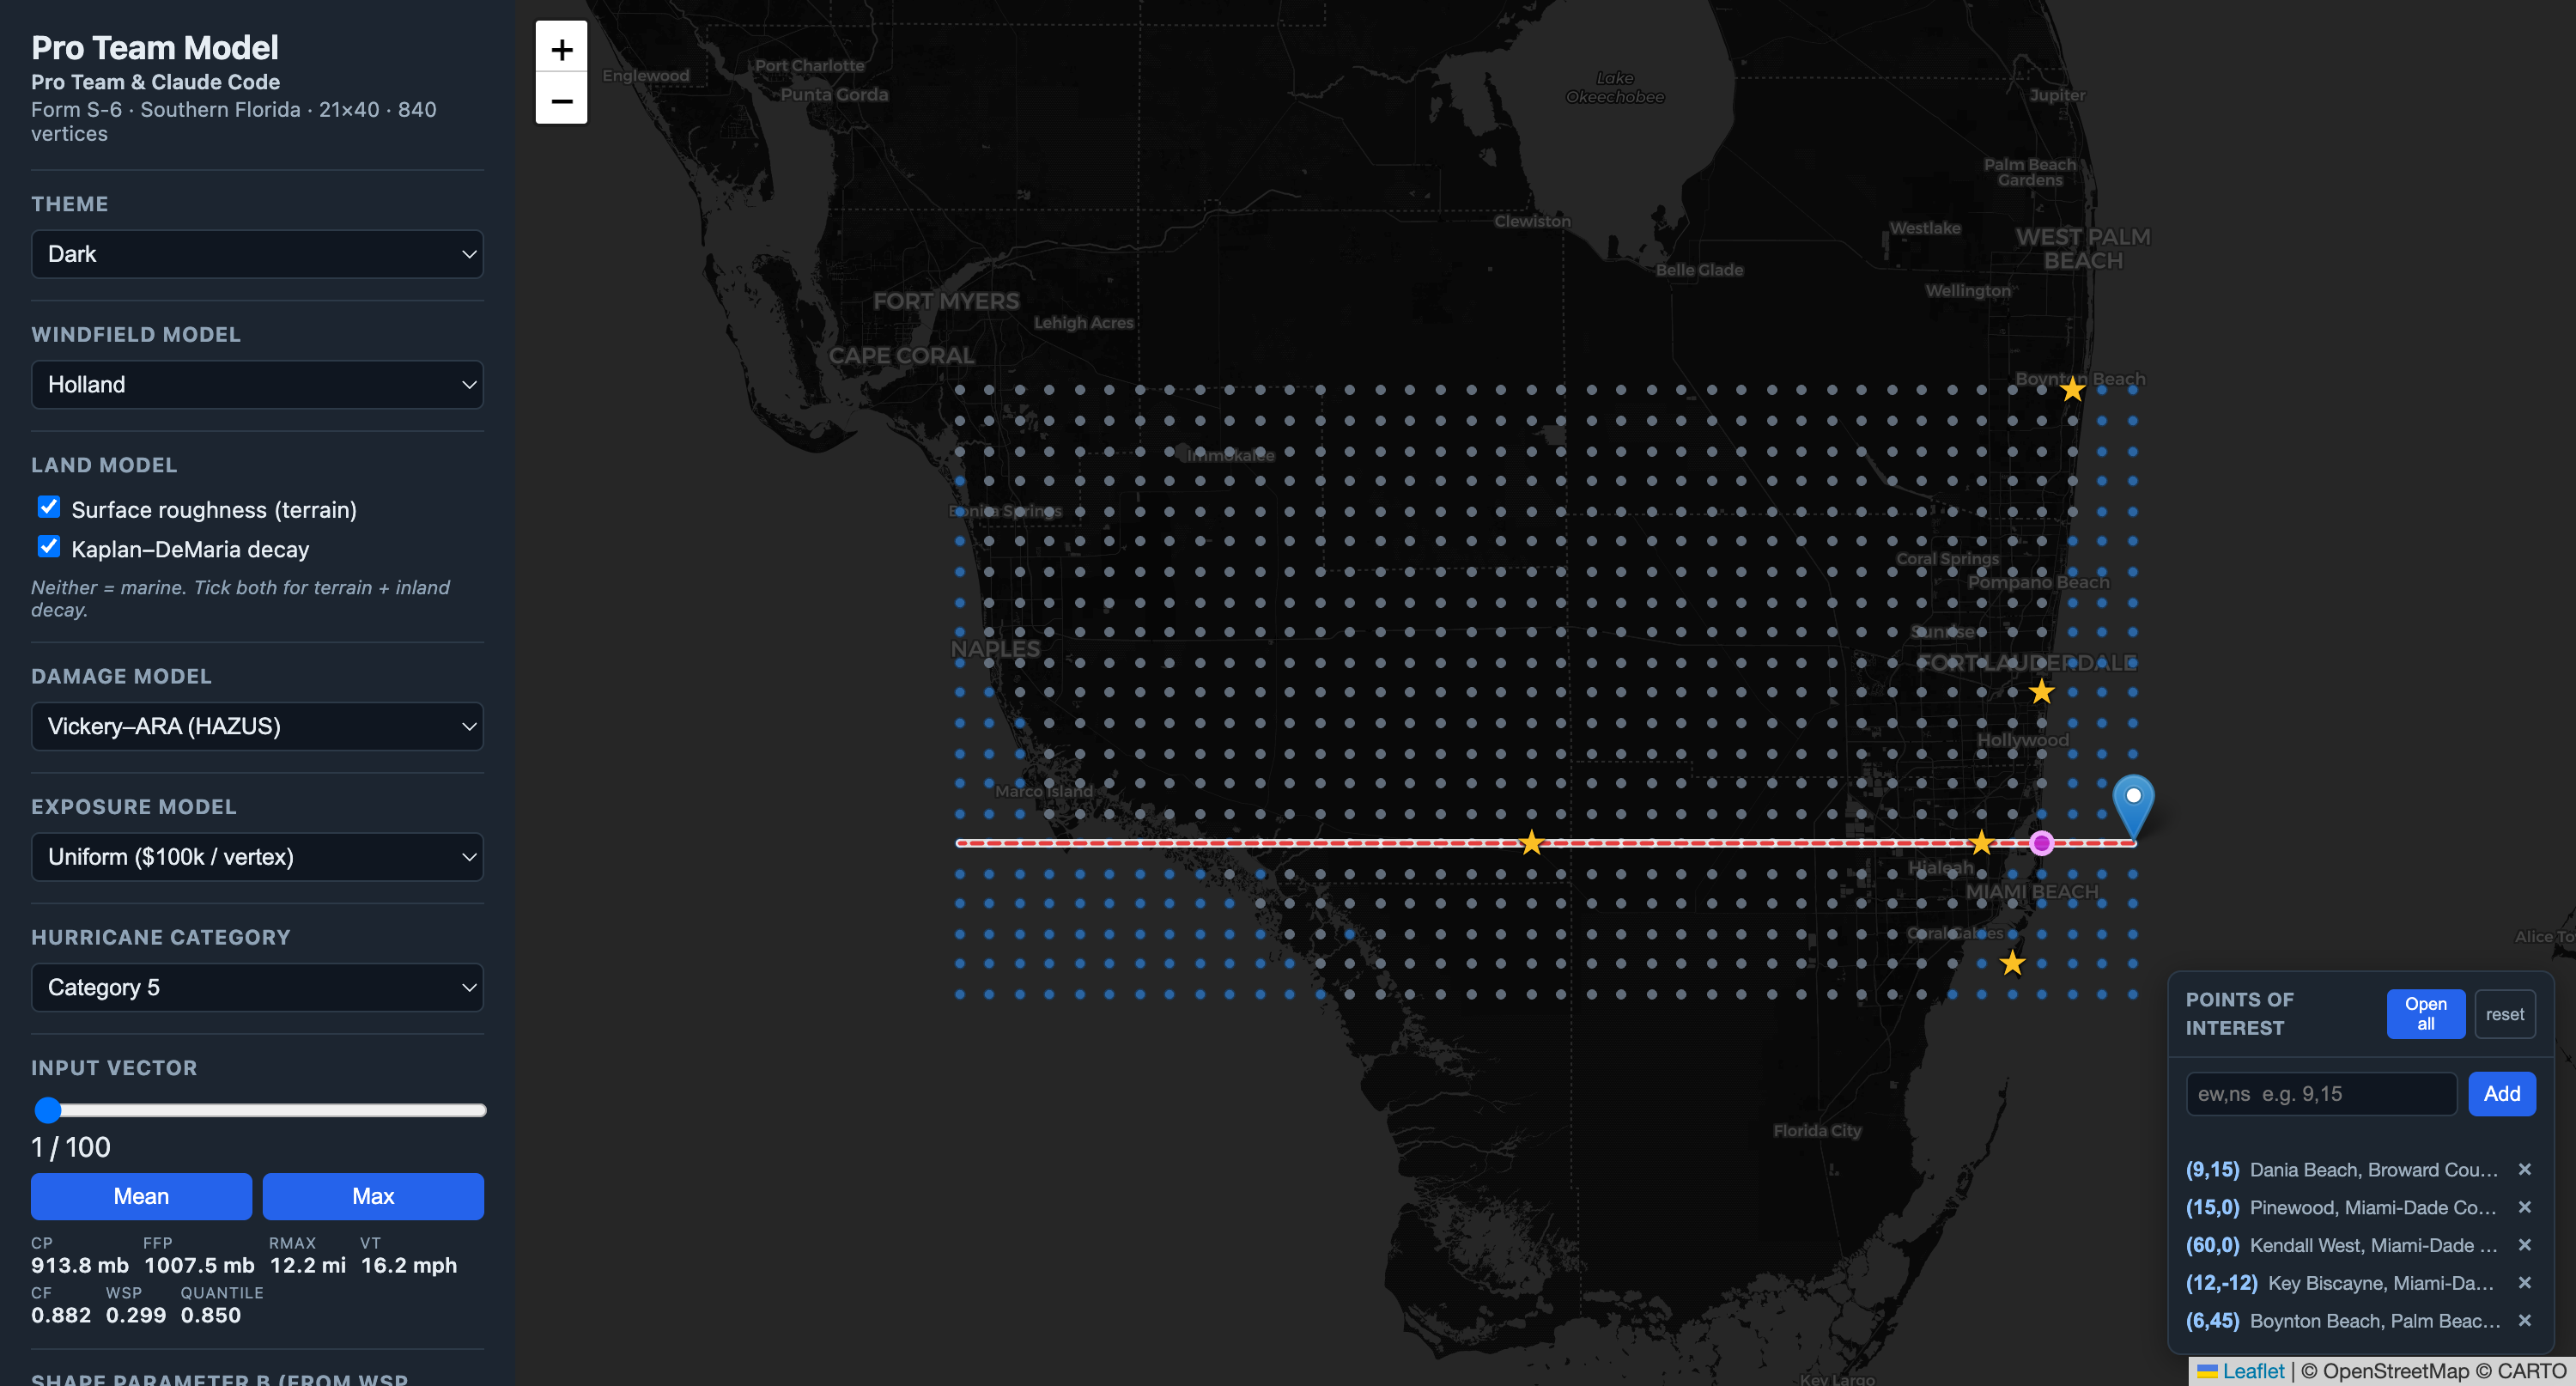
\includegraphics[width=\textwidth]{grid_basemap.png}
\caption{The 840-vertex Form S-6 grid over southern Florida: land (grey) and
water (blue) vertices, the due-west storm track (dashed), the $t\!=\!0$ centre,
and the landfall marker.}
\label{fig:grid}
\end{figure}

\subsection{Time step and grid-point loss convergence}
Each vertex's peak wind is the maximum over the passage as the (frozen)
storm-relative field advects across it; the boundary-layer PDE is solved
\emph{once} per storm and only this sampling is repeated per step, so a fine step
is nearly free. Because the spatial grid is coarse ($\sim$3\,mi), the
\emph{temporal} sampling carries the resolution of the peak: at hourly steps the
centre jumps $\text{VT}\times1\,\text{h}\approx13$--$16$\,mi---comparable to or
larger than Rmax---so the discrete samples can stride past the eyewall and miss
the true peak. The model uses a \textbf{1-minute step}
($T_{\Delta}=\tfrac{1}{60}$\,h; 2{,}161 steps over the 36-h window), at which the
peak is fully resolved.

Figure~\ref{fig:dtconv} quantifies the loss error from coarser steps relative to
the 1-min reference (HAZUS/ARA vulnerability curve, mean of 10 vectors per
category). \textbf{Hourly} stepping underestimates total loss by
$\approx$10\% (Cat~1), 3\% (Cat~3), and 1.5\% (Cat~5), and underestimates the
\emph{worst individual grid-point} loss by up to $\approx$42\% (Cat~1). The
effect is largest for the weaker storms, whose winds sit on the steep part of the
vulnerability curve so wind errors translate directly into loss errors---directly
relevant to the large point-to-point loss differences in the Cat~1/Cat~3 groups.
Loss is essentially converged by $\sim$2\,min; the 1-min step leaves no aliasing
and protects the worst individual vertices. Modelers stepping on synoptic
(hourly or 6-hourly) best-track cadence over a grid this coarse can therefore
materially under-report loss.

\begin{figure}[H]
\centering
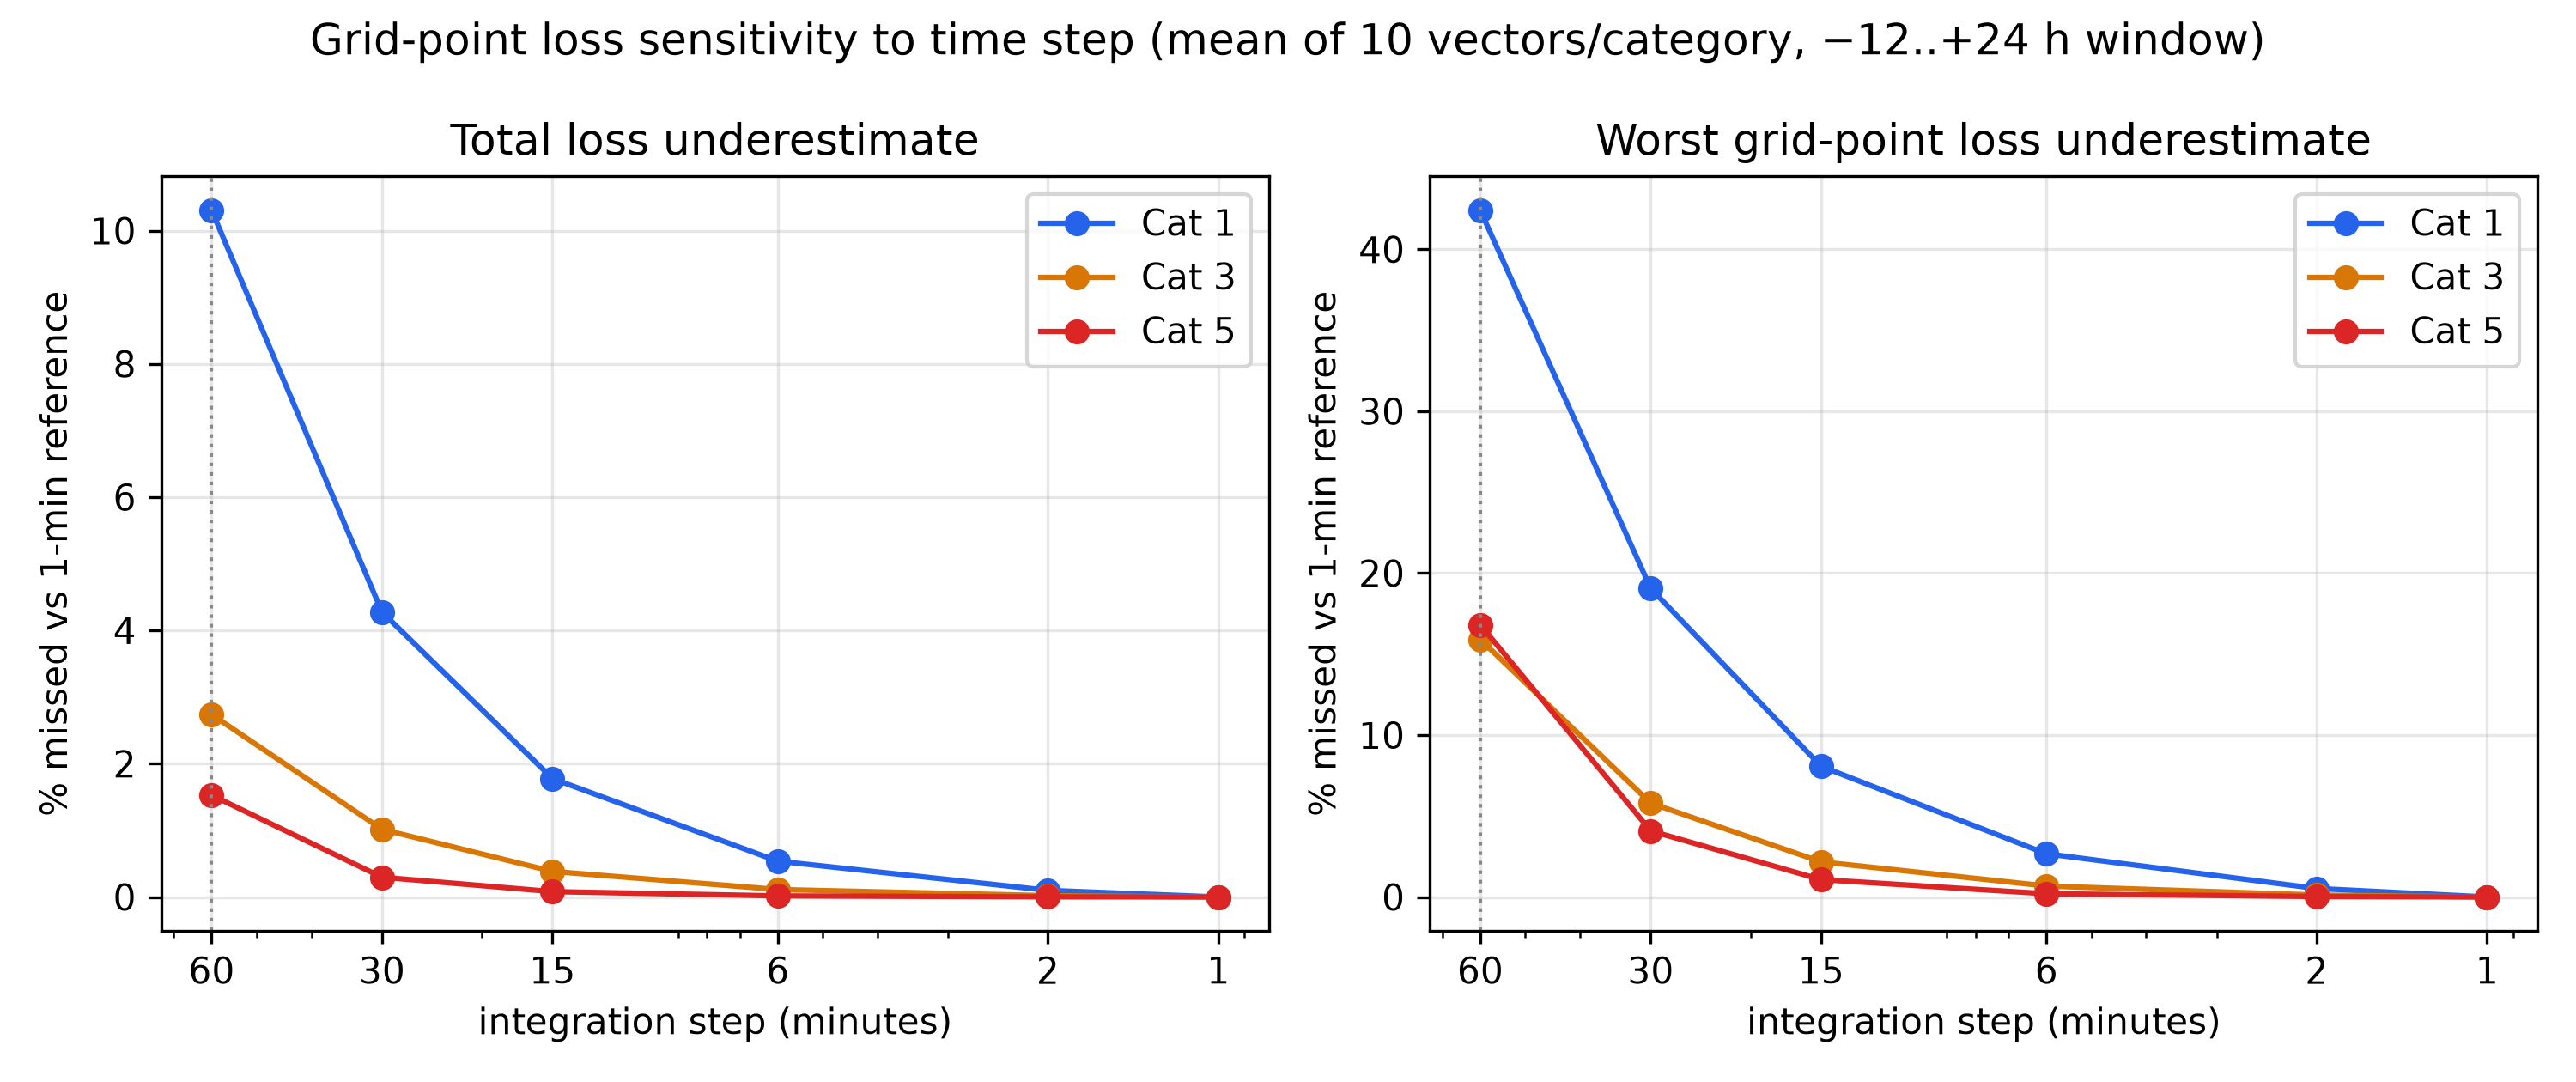
\includegraphics[width=\textwidth]{dt_convergence.png}
\caption{Grid-point loss sensitivity to integration step (hourly $\to$ 1-min),
as \% underestimate vs.\ the 1-min reference: total loss (left) and worst single
grid-point loss (right), per hurricane category. The dotted line marks hourly
stepping. The 1-minute step used by the model is fully converged.}
\label{fig:dtconv}
\end{figure}

\section{Meteorology: Wind-field models}
Three wind-field models are provided, each evaluated at all 840 vertices.
\textbf{Powell} is an iterative boundary-layer PDE (slab) solver;
\textbf{Holland} is the closed-form gradient-wind profile; \textbf{Willoughby}
is a piecewise power-law profile anchored to the Holland $V_{\max}$. All three
include translation asymmetry from the storm motion. All three footprint
windfields are \textbf{precomputed} so switching models is an instant lookup:
Powell via the Python PDE solver (\texttt{windfield\_grid.py}, PyTorch/MPS,
$\sim$2.3\,s per solve), and Holland/Willoughby by dumping the same closed-form
field code the viewer uses (\texttt{precompute\_live.py}), which keeps the
precomputed values identical to the live physics. The closed-form Holland and
Willoughby code is retained for the single-point profiler and the pop-up isotach,
which evaluate one vertex at a time.

Per-vector inputs come from the \texttt{SA all Variables} worksheet: central
pressure CP, radius of maximum wind Rmax, translation speed VT, wind-field shape
parameter WSP, conversion factor CF, and far-field pressure FFP, for 100 vectors
in each of categories 1, 3, and 5. The pressure deficit is $\Delta p=\text{FFP}-\text{CP}$.
WSP is supplied as a quantile $p\in[0,1]$ and mapped to the Holland shape
parameter $B$ through a user-selectable distribution (default Uniform$[1.0,2.5]$,
$B=B_{\min}+p\,(B_{\max}-B_{\min})$).

\paragraph{Conversion factor (CF).}
The ROA CF variable converts modelled gradient winds to surface winds using a
three-zone radial rule (ROA pp.~184--185): for $r<R_{\max}$,
$\text{CF}_{\text{eff}}=\text{CF}\cdot r/R_{\max}$; for
$R_{\max}\!<\!r\!<\!3R_{\max}$, $\text{CF}_{\text{eff}}=\text{CF}-0.1\,(r-R_{\max})/(2R_{\max})$;
and for $r>3R_{\max}$, $\text{CF}_{\text{eff}}=\text{CF}-0.1$. The models are run
at gradient level ($\beta_{10}=1$) and CF performs the gradient$\to$surface
conversion exactly as specified.

\paragraph{Peak-wind metric and time sampling.}
For each vector we record the per-vertex \textbf{peak surface wind} over the full
$-12$\,h\,$\to\,+24$\,h passage. The storm position is sampled at a 1-minute step
($\Delta t=\tfrac{1}{60}$\,h); coarser sampling aliases the fast westward motion
and under-resolves the peak (quantified in Figure~\ref{fig:dtconv}).
Figures~\ref{fig:powellpts} and \ref{fig:contours} show the peak field as coloured
points and as filled contours.

\begin{figure}[H]
\centering
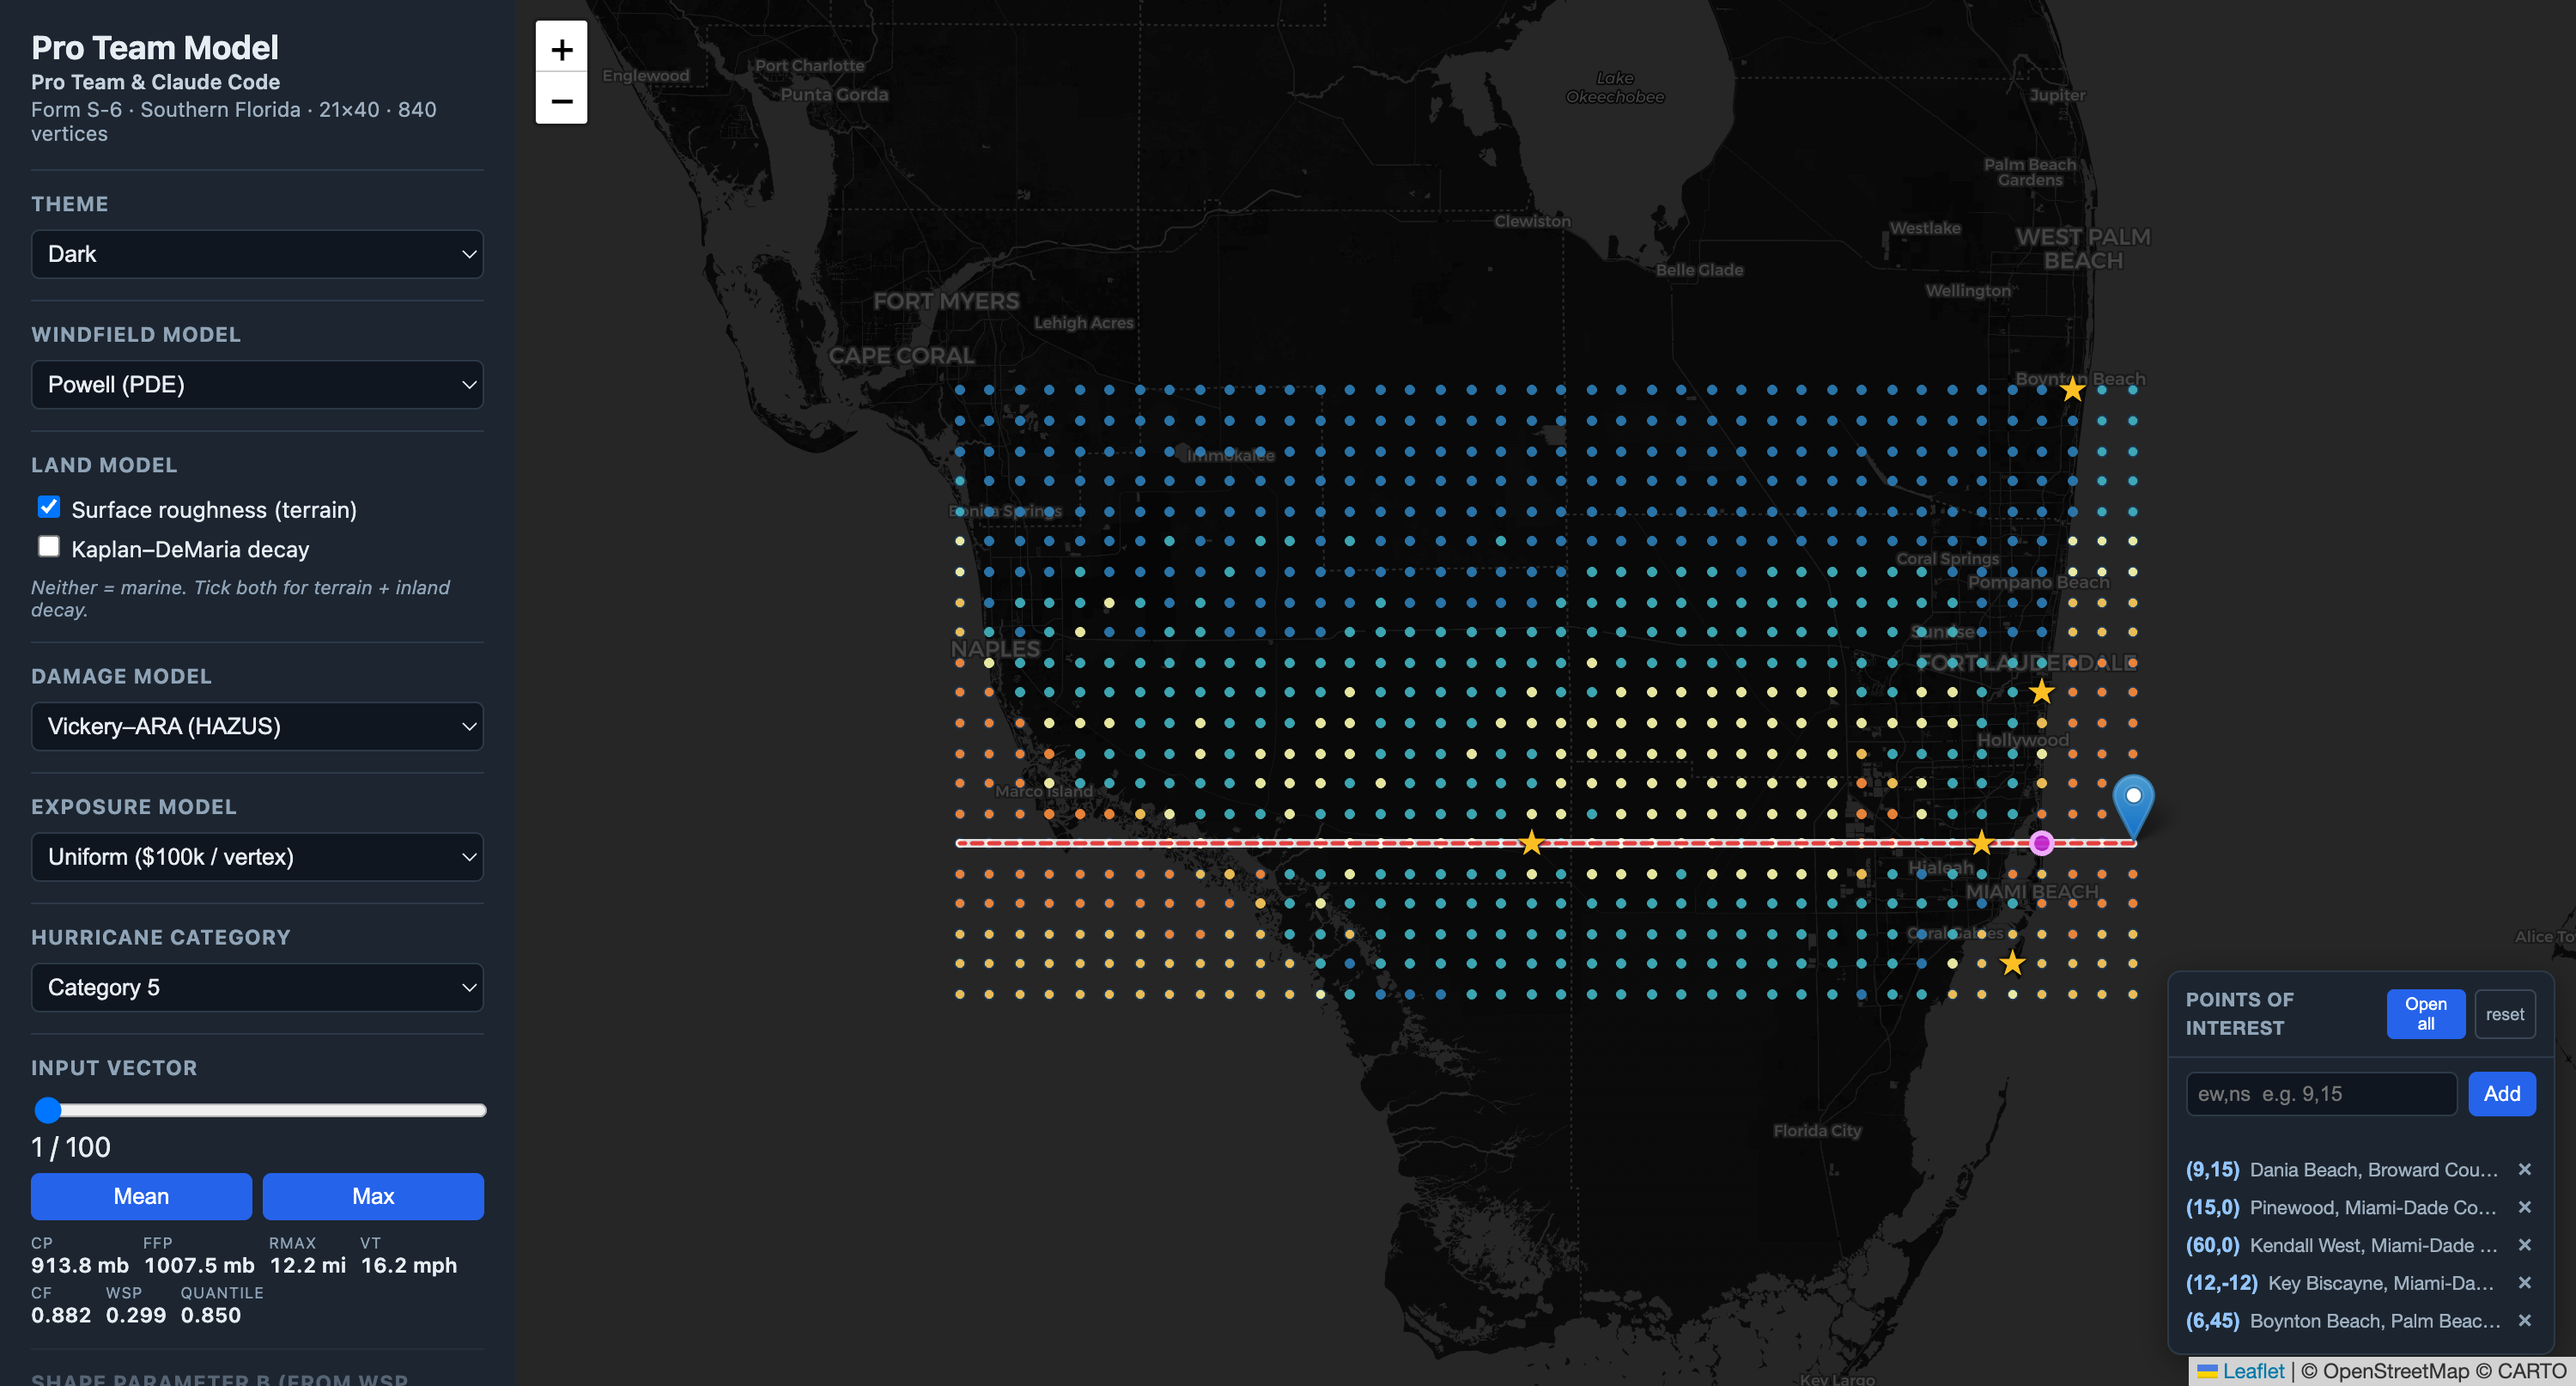
\includegraphics[width=\textwidth]{powell_cat5_pts.png}
\caption{Powell peak surface wind (Category 5, vector 1) coloured per vertex,
with surface roughness applied. Strongest winds lie north of the track---correct
for a westward-moving Northern-Hemisphere cyclone, where translation adds to
rotation on the north side.}
\label{fig:powellpts}
\end{figure}

\begin{figure}[H]
\centering
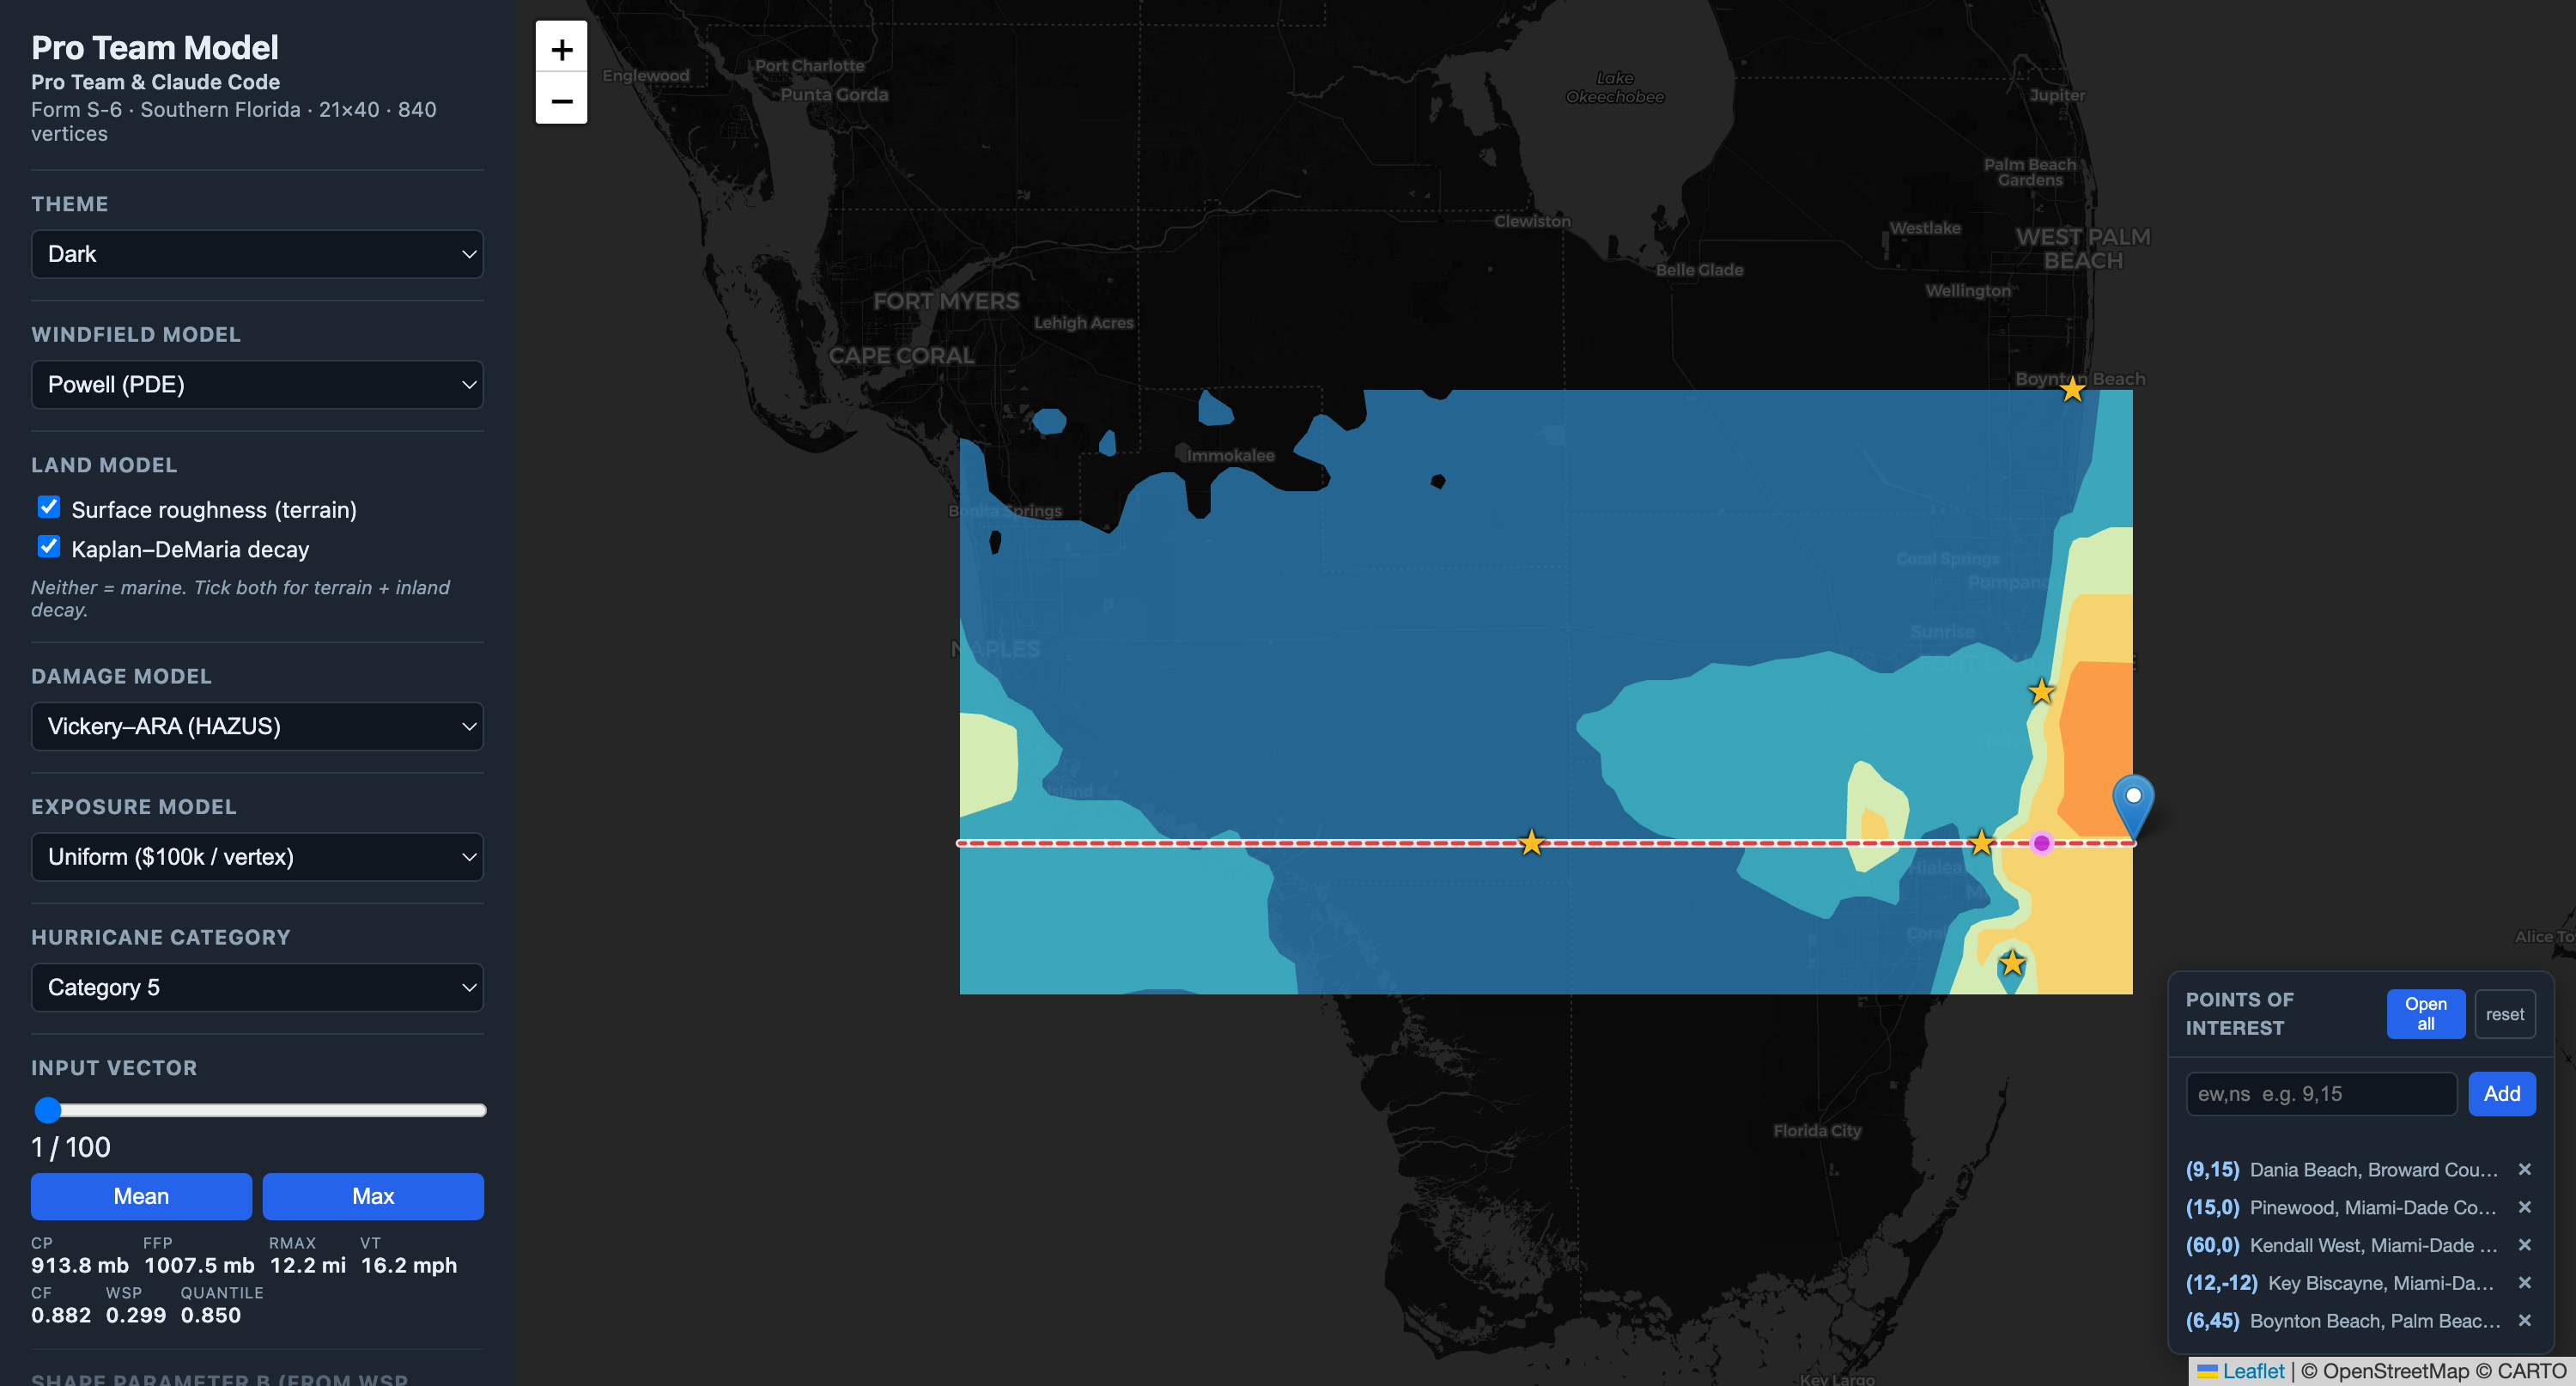
\includegraphics[width=0.49\textwidth]{powell_cat5_contour.png}\hfill
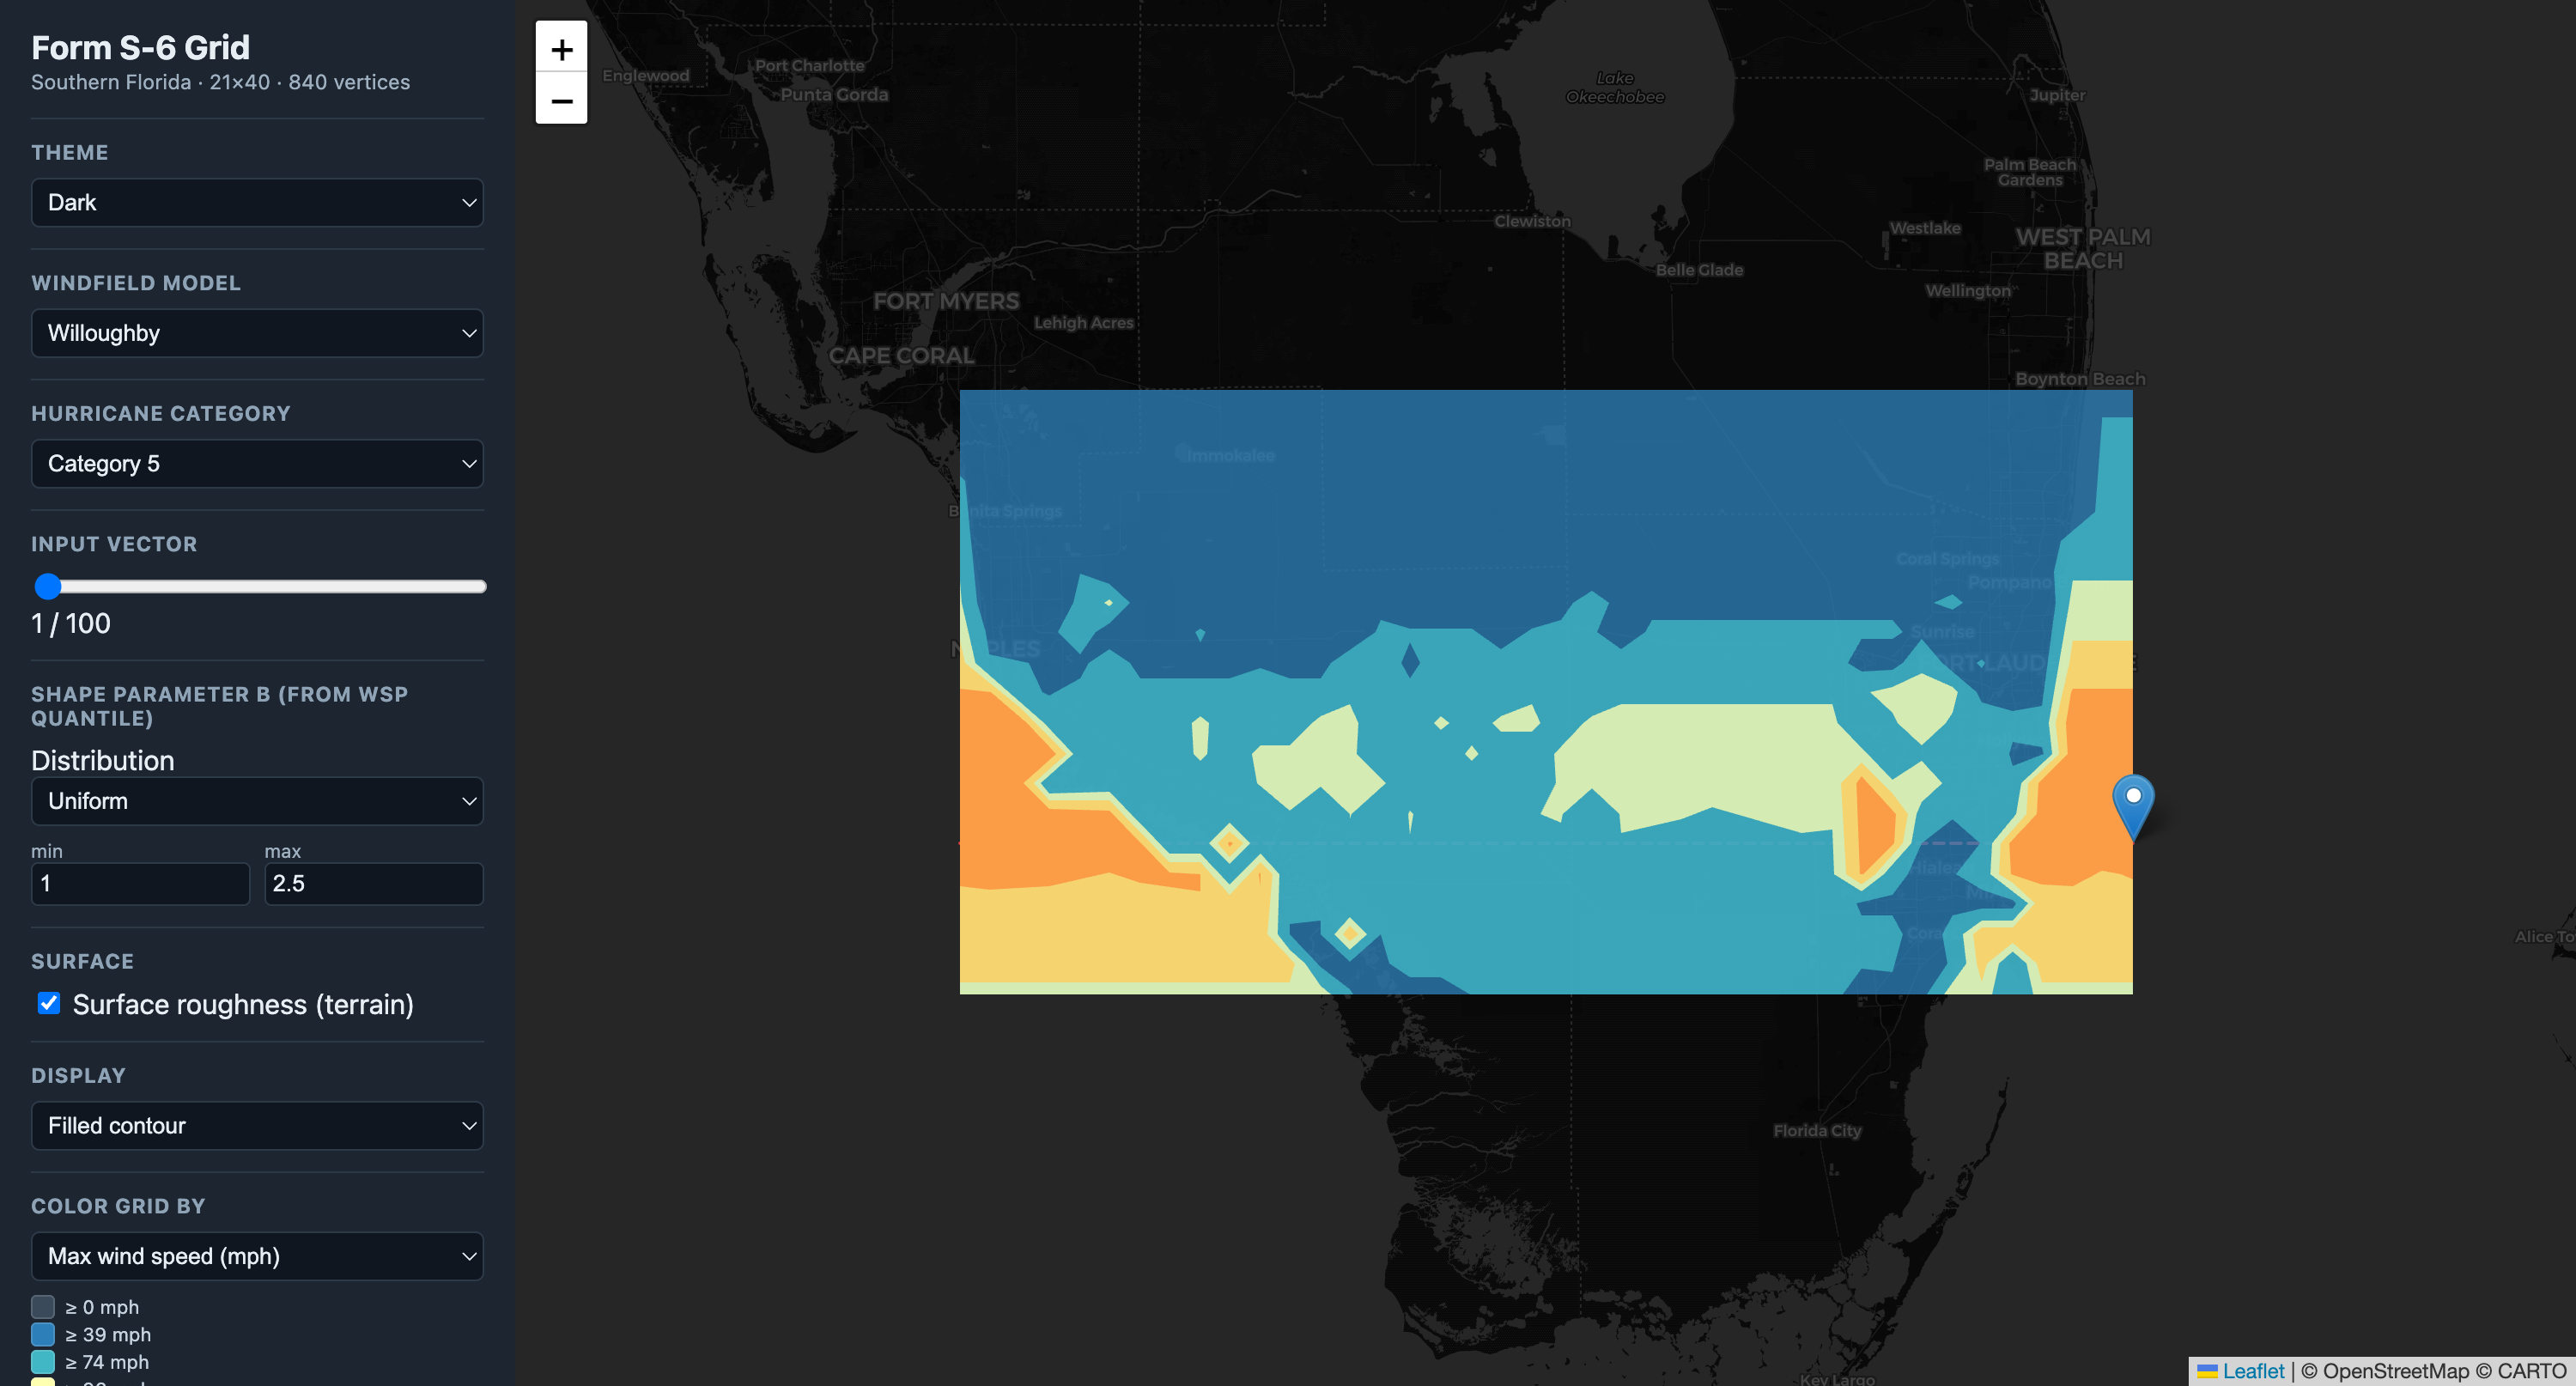
\includegraphics[width=0.49\textwidth]{willoughby_cat5_contour.png}
\caption{Filled-contour display (ROA Figs.~6--8 style) of the Category 5 peak
field: Powell (left) and Willoughby (right). To avoid faceted bands on the coarse
$21\times40$ lattice, the field is bilinearly upsampled and lightly smoothed before
the marching-squares contouring; the same treatment is applied to the pop-up
isotach plot.}
\label{fig:contours}
\end{figure}

\subsection{Numerical methods}\label{sec:numerics}
All three models produce a \emph{storm-relative} wind field that is then rigidly
advected across the grid (below); they differ only in \emph{how that field is
obtained}.

\paragraph{Closed-form profiles (Holland, Willoughby).}
Both rest on the gradient-wind balance, a quadratic in the wind speed $V$ that is
solved in \emph{closed form} by the quadratic formula---no iteration and no
numerical integration; the only ``root'' is analytic:
\[
V^2 + f r\,V - \frac{r}{\rho}\frac{dp}{dr}=0
\;\Longrightarrow\;
V(r)=\tfrac12\!\left(-f r + \sqrt{(f r)^2 + \tfrac{4r}{\rho}\tfrac{dp}{dr}}\,\right).
\]
\textbf{Holland}~\cite{holland} takes $dp/dr$ from its radial pressure profile
$p(r)=p_c+\Delta p\,e^{-(R_{\max}/r)^B}$, giving $V_g(r)$ directly.
\textbf{Willoughby}~\cite{willoughby} anchors $V_{\max}$ with the same formula at
$r=R_{\max}$ and then evaluates a piecewise analytic profile---an inner power law
$V_{\max}(r/R_{\max})^{n}$ and an outer decay $V_{\max}(r/R_{\max})^{-m}$---blended
by a logistic transition. Being pure algebra, both are cheap enough to evaluate
\emph{live} in the browser one vertex at a time (\texttt{web/windfield.js}); this is
what the single-point profiler and the pop-up isotach use.

\paragraph{Powell: a steady boundary-layer PDE.}
Powell~\cite{powell,vickery} instead solves the steady, depth-averaged (slab)
boundary-layer momentum equations for the horizontal wind $\mathbf u=(u,v)$ on a
radially-stretched polar grid ($N_r=200$, $N_\phi=360$):
\[
\frac{\partial \mathbf u}{\partial t}
= -(\mathbf u\!\cdot\!\nabla)\mathbf u
  \;-\; f\,\hat{\mathbf z}\times\mathbf u
  \;-\; \frac{1}{\rho}\nabla p
  \;+\; K_h\nabla^2\mathbf u
  \;-\; \frac{C_d\,|\mathbf U_{10}|}{h_{bl}}\,\mathbf u ,
\]
i.e.\ nonlinear advection (with the centrifugal $-v^2/r$ term), the Coriolis force,
the pressure-gradient force from the same Holland radial profile, horizontal
turbulent diffusion $K_h\nabla^2$, and a wind-dependent surface drag
$C_d(|\mathbf U_{10}|)$. The solver is \emph{not} a root-finder: it \textbf{marches
in pseudo-time to steady state} (relaxation / pseudo-transient continuation),
\[
\mathbf u \leftarrow \mathbf u + \Delta t\,\mathbf R(\mathbf u),\qquad
\Delta t=\min\!\Big(\text{CFL}\,\tfrac{\Delta x}{|\mathbf U|},\;
0.22\,\tfrac{\Delta x^2}{K_h},\;3\,\text{s}\Big),
\]
for $\sim$800 explicit steps with a CFL-limited adaptive step (advective and
diffusive stability), no-slip at the centre and an outer boundary relaxed toward
gradient balance. The converged field is the \emph{equilibrium} (mature-storm)
structure---a single steady field, not a time snapshot---to which the translation
vector is added for the earth-relative wind. At $\sim$2.3\,s per solve (PyTorch/MPS,
\texttt{hurricane\_pde\_marine.py}) this is far too costly for the browser, so the
$100$ vectors $\times$ $3$ categories are solved \emph{offline}
(\texttt{pipeline/windfield\_grid.py}) and only \emph{sampled} at run time---which is
why Powell single-point sensitivity uses a per-vertex metamodel
(Section~\ref{sec:metamodel}) rather than a live re-solve.

\paragraph{Frozen-field advection (shared by all three).}
Each model yields \emph{one} storm-relative field; the footprint is built by
translating that frozen field due west at the storm speed. With the eye at
$\mathrm{ew}_c=V_T t$, each vertex's storm-relative radius and azimuth $(r,\phi)$ are
formed, the frozen field is sampled there (bilinearly, for Powell), converted to the
surface with CF, and the per-vertex \emph{maximum} over $t\in[-12,+24]$\,h is kept.
The vortex \emph{structure} never evolves during the passage---the only
time-dependence is the translation itself (dominant), the optional Kaplan--DeMaria
intensity decay applied as a scalar $s(t)$ after landfall (magnitude, not shape),
and surface roughness (a per-vertex terrain factor fixed in the ground frame). This
is the standard steady-translating-vortex assumption for wind footprints, and it is
exactly what the optional storm animation (Figure~\ref{fig:anim}) makes visible.

\subsection{Powell (dynamic): a physical-time simulation}\label{sec:powelldyn}
The viewer's \textbf{Powell (dynamic)} option drops the frozen-field assumption: the
same slab boundary-layer momentum equations are integrated onward in \emph{physical}
time while the forcing evolves during the coastal crossing
(\texttt{pde\_dynamic\_marine} in the solver; batched precompute
\texttt{windfield\_dynamic\_batch.py}; forcing updated every $\Delta t=1$\,min).
Kaplan--DeMaria decay acts through the \emph{pressure} forcing
($\Delta p(t)=\Delta p_0\,s(t)^2$), so the wind follows the decay target with its
physical boundary-layer lag ($\tau\!\sim\!1$\,h) instead of instantaneously; the
Roughness option replaces none of the local exposure conversion but adds the
\emph{storm-scale} momentum sink: the drag coefficient under each node follows the
NLCD $z_0$ of the ground the storm is actually over ($C_d$ log-law over land,
Large--Pond over water), azimuthally asymmetric at landfall.

Long integration required two numerical corrections, applied only in the dynamic
tendency function (\texttt{physics\_terms\_dyn}; the steady Powell path is
byte-identical to before): (i) corrected Coriolis signs ($+fv$ radial, $-fu$
tangential; the flipped signs render a cyclone inertially unstable with a measured
$\sim$2$\times$10$^3$\,s e-fold, invisible in the 800-iteration steady solve but
fatal over hours --- effect on the steady product $\le$0.15\,mph), and (ii)
first-order upwind \emph{radial} advection, which captures the slab boundary-layer
inflow shock (Smith and Vogl 2008)~\cite{smithvogl} that blows up centred differences at
$\sim$8$\times$10$^3$\,s. The dynamic march starts from a spin-up run to true
convergence and was validated by regression: under constant marine forcing the
dynamic footprint equals the frozen-field translation \emph{exactly} (0.0\,mph at
every land vertex).

\paragraph{Baseline and tail behaviour (read before comparing models).}
Two deliberate differences from the steady Powell product must be understood when
comparing footprints. \emph{Baseline}: the production steady solve stops at 800
iterations ($\approx$48\,s of pseudo-time) --- a lightly relaxed initial guess ---
whereas the dynamic model must start from the true converged equilibrium of the same
equations, which is systematically stronger (cat3 example: 103.6 vs 96.6\,mph peak;
mean vertex difference 8.5\,mph). \emph{Tails}: this convergence gap grows with
storm intensity and tightness, because the unconverged production field is farthest
from equilibrium for small-$R_{\max}$, deep-$\Delta p$ vortices. Across the 300
input vectors the per-vector peak median is 138\,mph (dynamic) vs 124\,mph
(production), but the extreme tail --- vectors drawn near the input-distribution
edges, e.g.\ $R_{\max}\!\approx\!9$\,mi at $\mathrm{CP}\!\approx\!905$\,mb ---
reaches 280\,mph dynamic-marine vs 212\,mph production ($\approx$+30\%), and up to
346\,mph in the dynamic-roughness variants, where the sudden drag increase at
landfall drives a transient super-gradient boundary-layer jet (a real slab-model
phenomenon, amplified on already-extreme vectors). These values are faithful
equilibria of the Powell slab equations under Form S-6's unbounded input sampling,
not numerical failures. The model contains no thermodynamic ceiling---intensity is
an \emph{input} (CP, $R_{\max}$, WSP fix a pressure gradient that never weakens over
water), so over low-drag marine surfaces the boundary layer spins up to whatever
wind balances that prescribed forcing; nothing like a potential-intensity limit,
ocean-heat feedback, or eyewall replacement can intervene. The extreme values sit
far above any observed surface wind and should be read as tail artefacts of the
input distribution, not as forecasts. The four precomputed products
(\texttt{powell\_dyn\{,\_kd,\_rough,\_kd\_rough\}.json}) cover the
decay$\times$roughness checkbox states; Powell (dynamic) provides peak footprints
only (no storm-relative popup series or animation --- the field is no longer
translation-invariant), and the \textbf{Powell (steady)} option is retained
unchanged as the reference. The two are labelled \emph{steady} and \emph{dynamic}
rather than ``PDE'' and ``dynamic'': both solve the same slab boundary-layer PDE,
and what separates them is whether it is integrated in time.

\section{Meteorology: Land effect---roughness and decay}
The storm's interaction with the land is modelled by two \emph{independent},
combinable toggles: \textbf{Surface roughness} and \textbf{Kaplan--DeMaria
decay}~\cite{kaplan}. They are checkboxes rather than a single exclusive selector, so all four
states are reachable: neither (pure marine winds), either alone, or both
together. The default is \textbf{both on}: a spatial terrain-friction effect plus
a temporal inland-filling effect, which together give the most physically
realistic field (see below).

\paragraph{Surface roughness.}
Roughness is applied as a per-vertex, wind-speed-independent multiplier on the
final surface wind. The roughness length $z_0$ at each vertex is derived from
\textbf{NLCD~2021 land cover}~\cite{nlcd} (fetched as a properly georeferenced GeoTIFF from
the MRLC WCS) via a published land-cover$\to z_0$ table~\cite{aersurface}, then converted from
marine to terrain exposure with the gradient-tied \textbf{log-law}
(Vickery et al.\ 2009 / ESDU)~\cite{vickery,esdu}, following the standard practice for
reducing hurricane surface winds to a common exposure~\cite{powell1996}:
\[
\text{factor}=\frac{\ln(z_{\text{ref}}/z_{0,\text{land}})/\ln(z_g/z_{0,\text{land}})}
{\ln(z_{\text{ref}}/z_{0,\text{marine}})/\ln(z_g/z_{0,\text{marine}})},
\]
with $z_{\text{ref}}=10$\,m and gradient height $z_g=500$\,m; water returns
$\approx1$. The land-mean factor is $\approx0.68$ (urban $\sim0.50$, wetland
$\sim0.70$). This is a \emph{spatial} terrain-friction effect.

\paragraph{Fetch-blended effective roughness.}
The effective $z_{0,\text{land}}$ at each vertex is not the single underlying
pixel but the \textbf{area-weighted geometric mean} (log-average) of the
per-pixel $z_0$ over a $\sim500$\,m window---the standard way to combine
heterogeneous roughness over an upwind fetch. This replaces an earlier
modal ``winner-take-all'' class, which could flip a coastal developed vertex
entirely to open water whenever the window happened to be water-dominated. The
blend yields smooth shoreline transitions (e.g.\ a bayfront suburban point
blends to $z_0\!\approx\!21$\,mm, factor~$\approx\!0.83$, rather than snapping to
$1.0$).

\paragraph{Per-vertex inspection.}
Hovering any grid vertex reports its \emph{exact-pixel} NLCD land cover together
with the fetch-blended $z_0$ (mm) and the resulting multiplier. This exposes
land/water coding discrepancies: a handful of vertices flagged \emph{land} in the
Form~S-6 grid fall on NLCD open water (e.g.\ the NW Miami-Dade ``Lake Belt''
limestone quarry lakes), so they carry exposure/loss on what is physically water.
Adjacent-vertex roughness differences---which can drive the large point-to-point
loss spread seen in the Cat~1/Cat~3 groups---are likewise directly inspectable.

\paragraph{Kaplan--DeMaria decay.}
Roughness alone cannot reproduce a storm weakening as it moves inland, which is
a \emph{temporal} filling process. The Kaplan--DeMaria (1995) model is offered as
a separate option: a one-time coastal reduction ($R=0.90$) at first landfall, then
$V(t)=V_b+(R\,V_0-V_b)\,e^{-\alpha t}$ with $\alpha=0.095\,\text{h}^{-1}$ and
background $V_b=30.7$\,mph over land, with a gentle recovery
($\alpha_{\text{rec}}=0.05\,\text{h}^{-1}$) once the centre re-emerges over the
Gulf. Landfall ($\approx$E-W~9) and Gulf exit ($\approx$E-W~99) are read from the
$N$-$S=0$ track land mask. Figure~\ref{fig:kdloss}~(left) shows the resulting
inland decay for a Category~5 storm. Roughness and decay compose multiplicatively
and are on by default: because the roughness factor is time-independent, the
combined peak equals (decayed peak)\,$\times$\,(roughness factor). With both
active the peak wind/loss returns to the coast---e.g.\ at a point $60$\,mi inland
over the Everglades the Cat~5 mean peak falls from $\approx\!158$\,mph (marine) to
$\approx\!78$\,mph---rather than persisting at full marine strength far inland.

\section{Vulnerability: Damage curves}\label{sec:vuln}
The ROA (p.~186) fixes a single insured structure at \emph{every} one of the 682
land vertices: a \$100{,}000, zero-deductible, single-family, single-story,
masonry, gable-roof, no-shutter home with truss anchors, shingles over 15\# felt,
a $\tfrac12$\,in.\ plywood deck (8d nails at 6\,in.\ edge / 12\,in.\ field), built
1995, roof age unknown---the wind-loss mitigation attributes characterized in
ARA's Florida wind-loss mitigation study \cite{araoir2024}. Because the structure
is uniform, a \textbf{single vulnerability curve} applies at all points and only
the wind varies.

The curve is generated from our existing HAZUS/ARA wind-vulnerability tool
(\texttt{wind\_\allowbreak vulnerability\_\allowbreak tool\_\allowbreak v5.html}),
a damage-state fragility model following the HAZUS hurricane methodology
\cite{hazus,vickery2006}, driven headlessly to the structure
above, yielding Mean Damage Ratio (MDR) versus the ASCE~7-98 3-second peak gust at
10\,m (Exposure~C). The resulting masonry curve (Figure~\ref{fig:vuln}) is a smooth
sigmoid: $\sim$0 below 50\,mph, 50\% near 100\,mph, and a plateau at MDR~$\approx
0.60$ above $\sim$140\,mph---the masonry ceiling (walls survive; roof, openings,
and contents bound the loss), in contrast to frame construction which approaches
1.0. In the sidebar this curve is identified by a \textbf{Damage model} selector
(\emph{Vickery--ARA (HAZUS)}\cite{hazus,vickery2006}, the default), placed directly under the wind-field
selector so that alternative vulnerability models can be added alongside it.

\paragraph{Logistic damage model (adjustable parameters).}
A second, \emph{parametric} damage model is provided as \textbf{Logistic}. Rather
than the tabulated HAZUS curve it uses a closed-form piecewise
logistic in the 3-second gust $v$ (mph),
\[
D(v)=\begin{cases}\dfrac{1}{1+e^{-k(v-v_{50})}} & v<v_{\max}\\[4pt] 1 & v\ge v_{\max}\end{cases}
\]
with three \emph{user-selectable} parameters exposed as inputs when the model is
chosen: the median capacity $v_{50}$ (the gust at which damage reaches 50\%), the
steepness $k$, and the total-loss gust $v_{\max}$. The defaults
($v_{50}=148$\,mph, $k=0.08$, $v_{\max}=180$\,mph) describe the reference
house---1995 masonry but with \emph{no shutters and a gable roof}: the open envelope
lets internal pressurization pop the gable roof off its anchors, so damage
progresses from a lower median than a sealed ``bunker'' and, unlike the masonry
curve (which plateaus near $0.60$), saturates to \emph{total} loss ($D=1$) by
$180$\,mph. Switching the damage model---or editing any parameter---re-renders the
loss map, \%TLC, financial panel, and the single-point loss responses live through
the same \texttt{mdrAt} used everywhere (the precomputed GPR/NN loss metamodels
encode the HAZUS curve, so under the logistic model the profiler's loss response
falls back to the live second-order fit).

\begin{figure}[H]
\centering
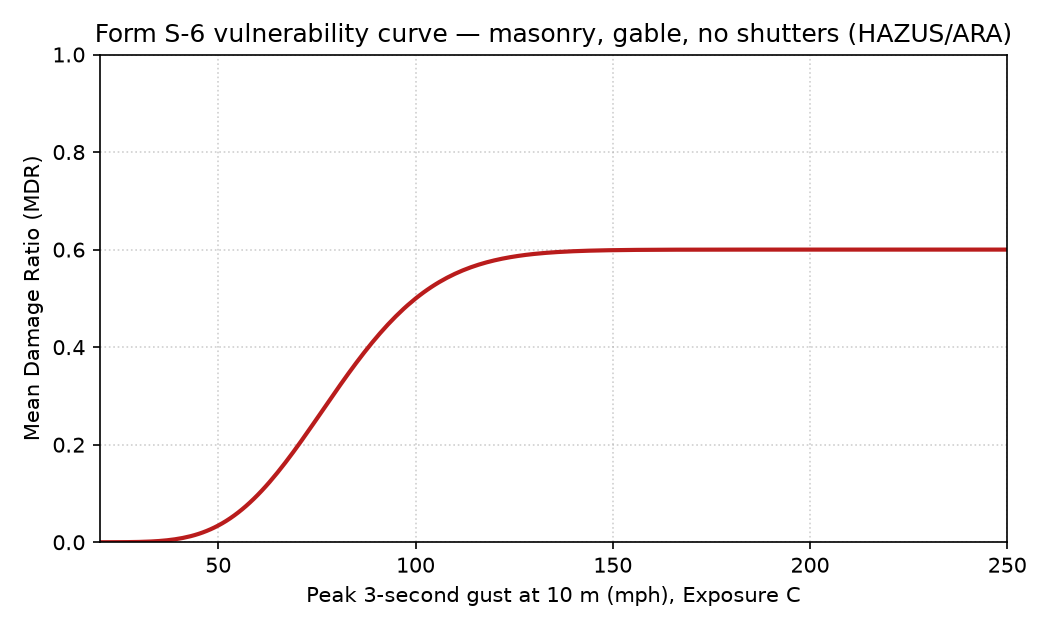
\includegraphics[width=0.7\textwidth]{vulnerability_curve.png}
\caption{Form S-6 vulnerability curve (Mean Damage Ratio vs.\ peak 3-second gust)
for the masonry, gable, no-shutter structure, generated from the HAZUS/ARA tool.}
\label{fig:vuln}
\end{figure}

\section{Actuarial: Loss Cost}\label{sec:loss}
Per-vertex loss is $\text{loss}=\text{MDR}(\text{peak wind})\times\text{exposure}_{x,y}$;
the expected loss as a percent of exposure is the total over the 682 land vertices
divided by the total exposure. The viewer colours the
grid by MDR, reports total loss and \% exposure, and the hover popup shows
loss \% and dollars beside the peak wind. Figure~\ref{fig:kdloss} shows Category~5
Kaplan--DeMaria-decayed wind (left) and the corresponding loss field (right).

Because the published HAZUS/ARA curve is a single-valued function of the
\emph{peak} gust, the loss reported here is peak-driven: two storms that reach the
same peak at a location score the same loss even if one holds the point above the
damage threshold far longer. Duration is embedded in the fragility curve at one
nominal storm speed rather than re-integrated per event; loss in reality
accumulates for as long as the wind stays elevated. Section~\ref{sec:metamodel}
therefore adds a location-level \emph{duration-of-exposure} diagnostic that
re-exposes the forward-speed and size dependence the peak metric collapses.

\paragraph{Duration-accumulated loss (rate-integrated MDR).}
As an explicit accumulated-damage alternative to the peak curve, a single-point
response integrates damage \emph{every timestep} the wind is above the threshold,
at the instantaneous-MDR rate:
\[
\mathrm{MDR}_{\mathrm{acc}}(x)=\min\!\Big(\tfrac1\tau\!\!\int_{V(t)\ge V_0}\!\!\!\!
\mathrm{MDR}\big(V(t)\big)\,dt,\ \ \mathrm{MDR}_{\max}\Big),\qquad V_0=40\ \text{mph},
\]
capped at the curve's plateau $\mathrm{MDR}_{\max}$. The reference exposure time
$\tau$ is calibrated \emph{per point} so the $100$-vector mean of
$\mathrm{MDR}_{\mathrm{acc}}$ equals the mean of the peak-based $\%\mathrm{LC}$: the
metric carries \emph{no net bias} against HAZUS, but \emph{redistributes} loss by
dwell---slow, large storms that linger accrue more, fast storms less. It is thus a
duration \emph{sensitivity} rather than a re-levelled loss, and it reduces to the
HAZUS value for a nominal-duration storm. At an off-track vertex, for example,
$\mathrm{MDR}_{\mathrm{acc}}$ \emph{falls} as forward speed $V_T$ rises (less dwell),
the opposite of the peak $\%\mathrm{LC}$ there (which rises with $V_T$ through the
stronger translation asymmetry)---the two agree only in the mean. Because it needs
the wind time series, it is a single-point, live-model response
(Holland/Willoughby); Powell, having no live field, shows a note.

\paragraph{Exposure model (the 4th module).}
Exposure---\emph{how much insured value sits at each location}---is the fourth
catastrophe-model leg alongside hazard, vulnerability, and finance, and the sidebar
exposes it as a swappable \textbf{Exposure model} selector under the damage model.
\emph{Uniform} is the ROA baseline: one identical \$100{,}000 home at every land
vertex, total $\$68.2$M. \emph{Census} replaces that with the \emph{actual}
aggregate home value in each vertex's 3-mile cell, built offline
(\texttt{pipeline/build\_exposure.py}) from the American Community Survey (ACS
5-year table B25082, aggregate owner-occupied value) areal-apportioned from Florida
TIGER tract polygons onto the grid (the heavy GIS stays in the pipeline; only a
small per-vertex JSON reaches the browser). For the Southern-Florida footprint the
Census total is $\approx\$572$B, and value is sharply concentrated---the densest
Miami cell carries $\sim$1500$\times$ the median cell---so loss becomes weighted by
\emph{where value actually is}, not merely by mean damage: $\%\text{TLC}$ for the
Category~5 example shifts from $28.3\%$ (Uniform) to $24.7\%$ (Census), and the
financial panel's AAL/return-period losses rescale from millions to billions. The
exposure model feeds the loss totals, the per-point CSV ($\%\text{TLC}$), the
CDF, and the financial panel consistently; per-point MDR (and hence the map
colouring) is exposure-independent.

\emph{Tax Roll (FL DOR)} is the third option, and it exists to fix a defect the first
two share. Loss is $\text{MDR}\times\text{exposure}$, where MDR is a \emph{structural}
damage ratio; but the ACS question asks what ``this house \emph{and lot}'' would sell
for, so Census exposure is land-inclusive and land cannot be separated out of it. Wind
does not damage land. Measured on the Florida Department of Revenue 2025 cadastral, land
is $41.3\%$ of single-family just value in this domain (and $59.1\%$ in Miami-Dade), so
a structural MDR applied to house-and-lot value overstates loss---worst on the expensive
coast, where the wind field is strongest. The error correlates with the hazard.

The roll separates them by statute (s.193.114 F.S.: $JV = LND\_VAL + \text{building} +
SPEC\_FEAT$), but a naive subtraction fails: county appraisers fold a condominium's land
into the unit's just value and report $LND\_VAL = 0$ for $99.9\%$ of condo parcels
($37\%$ of all residential parcels here, \$249B of just value, concentrated in the
coastal high-rises). We therefore build the basis a catastrophe model actually wants---
\emph{replacement cost}:
\[
\text{exposure(cell)} \;=\; r \times \!\!\sum_{\text{residential parcels}}\!\! \texttt{TOT\_LVG\_AR},
\qquad
r \;=\; \operatorname{median}\!\left(\frac{JV - LND\_VAL - SPEC\_FEAT}{\texttt{TOT\_LVG\_AR}}\right)_{\text{single family}}
\]
with $r=\$169.96$/sqft calibrated over $962{,}763$ single-family parcels---the clean
subset where the appraiser does separate land. Land is absent by construction and condos
and houses sit on one basis. Crucially $r$ is a \emph{single domain-wide constant}: a
per-county rate would encode land-\emph{allocation policy} rather than construction cost
(Broward assigns $9.1\%$ of just value to land, Miami-Dade $59.1\%$, at an identical
median market value of ${\sim}\$280$/sqft), imposing a spurious $2.3\times$ seam along
the county line that crosses this grid at ${\sim}25.96^\circ$N. Because
$\%\text{TLC}=\sum \text{MDR}\cdot\text{exposure}/\sum\text{exposure}$, a constant $r$
cancels exactly: $\%\text{TLC}$, SRC and EPR are invariant to it, and $r$ sets the dollar
totals only.

Each parcel is assigned to exactly one cell by its \emph{centroid}. The grid steps
exactly $3$\,mi in $ew$ and $ns$, so the 3-mile cells tile the domain: no parcel is
double-counted at a boundary, and---unlike tract-density apportionment---no value is
smeared onto water or the Everglades ($83\%$ of interior Everglades cells are correctly
empty under Tax Roll, against $232$ cells carrying spurious Census value). The domain
total is $\$619$B of replacement cost over $1{,}611{,}952$ residential parcels and
$3.64$B sqft of living area. That it \emph{exceeds} the \$572B Census total despite
excluding land is itself the second Census defect made visible: B25082 counts
owner-occupied units only, so it omits renter-occupied housing entirely.
(Caveats: assessed/taxable value is deliberately \emph{not} used---Save Our Homes caps
assessed growth at $3\%$/yr, so it diverges from market value; $r$ is calibrated on
low-rise masonry and applied to high-rise condo floor area, which likely
\emph{understates} high-rise replacement cost; commercial and vacant parcels are
excluded. Built offline by \texttt{pipeline/build\_exposure\_tax.py} from the statewide
cadastral fetched by \texttt{pipeline/fetch\_cadastral.sh}.)

\begin{figure}[H]
\centering
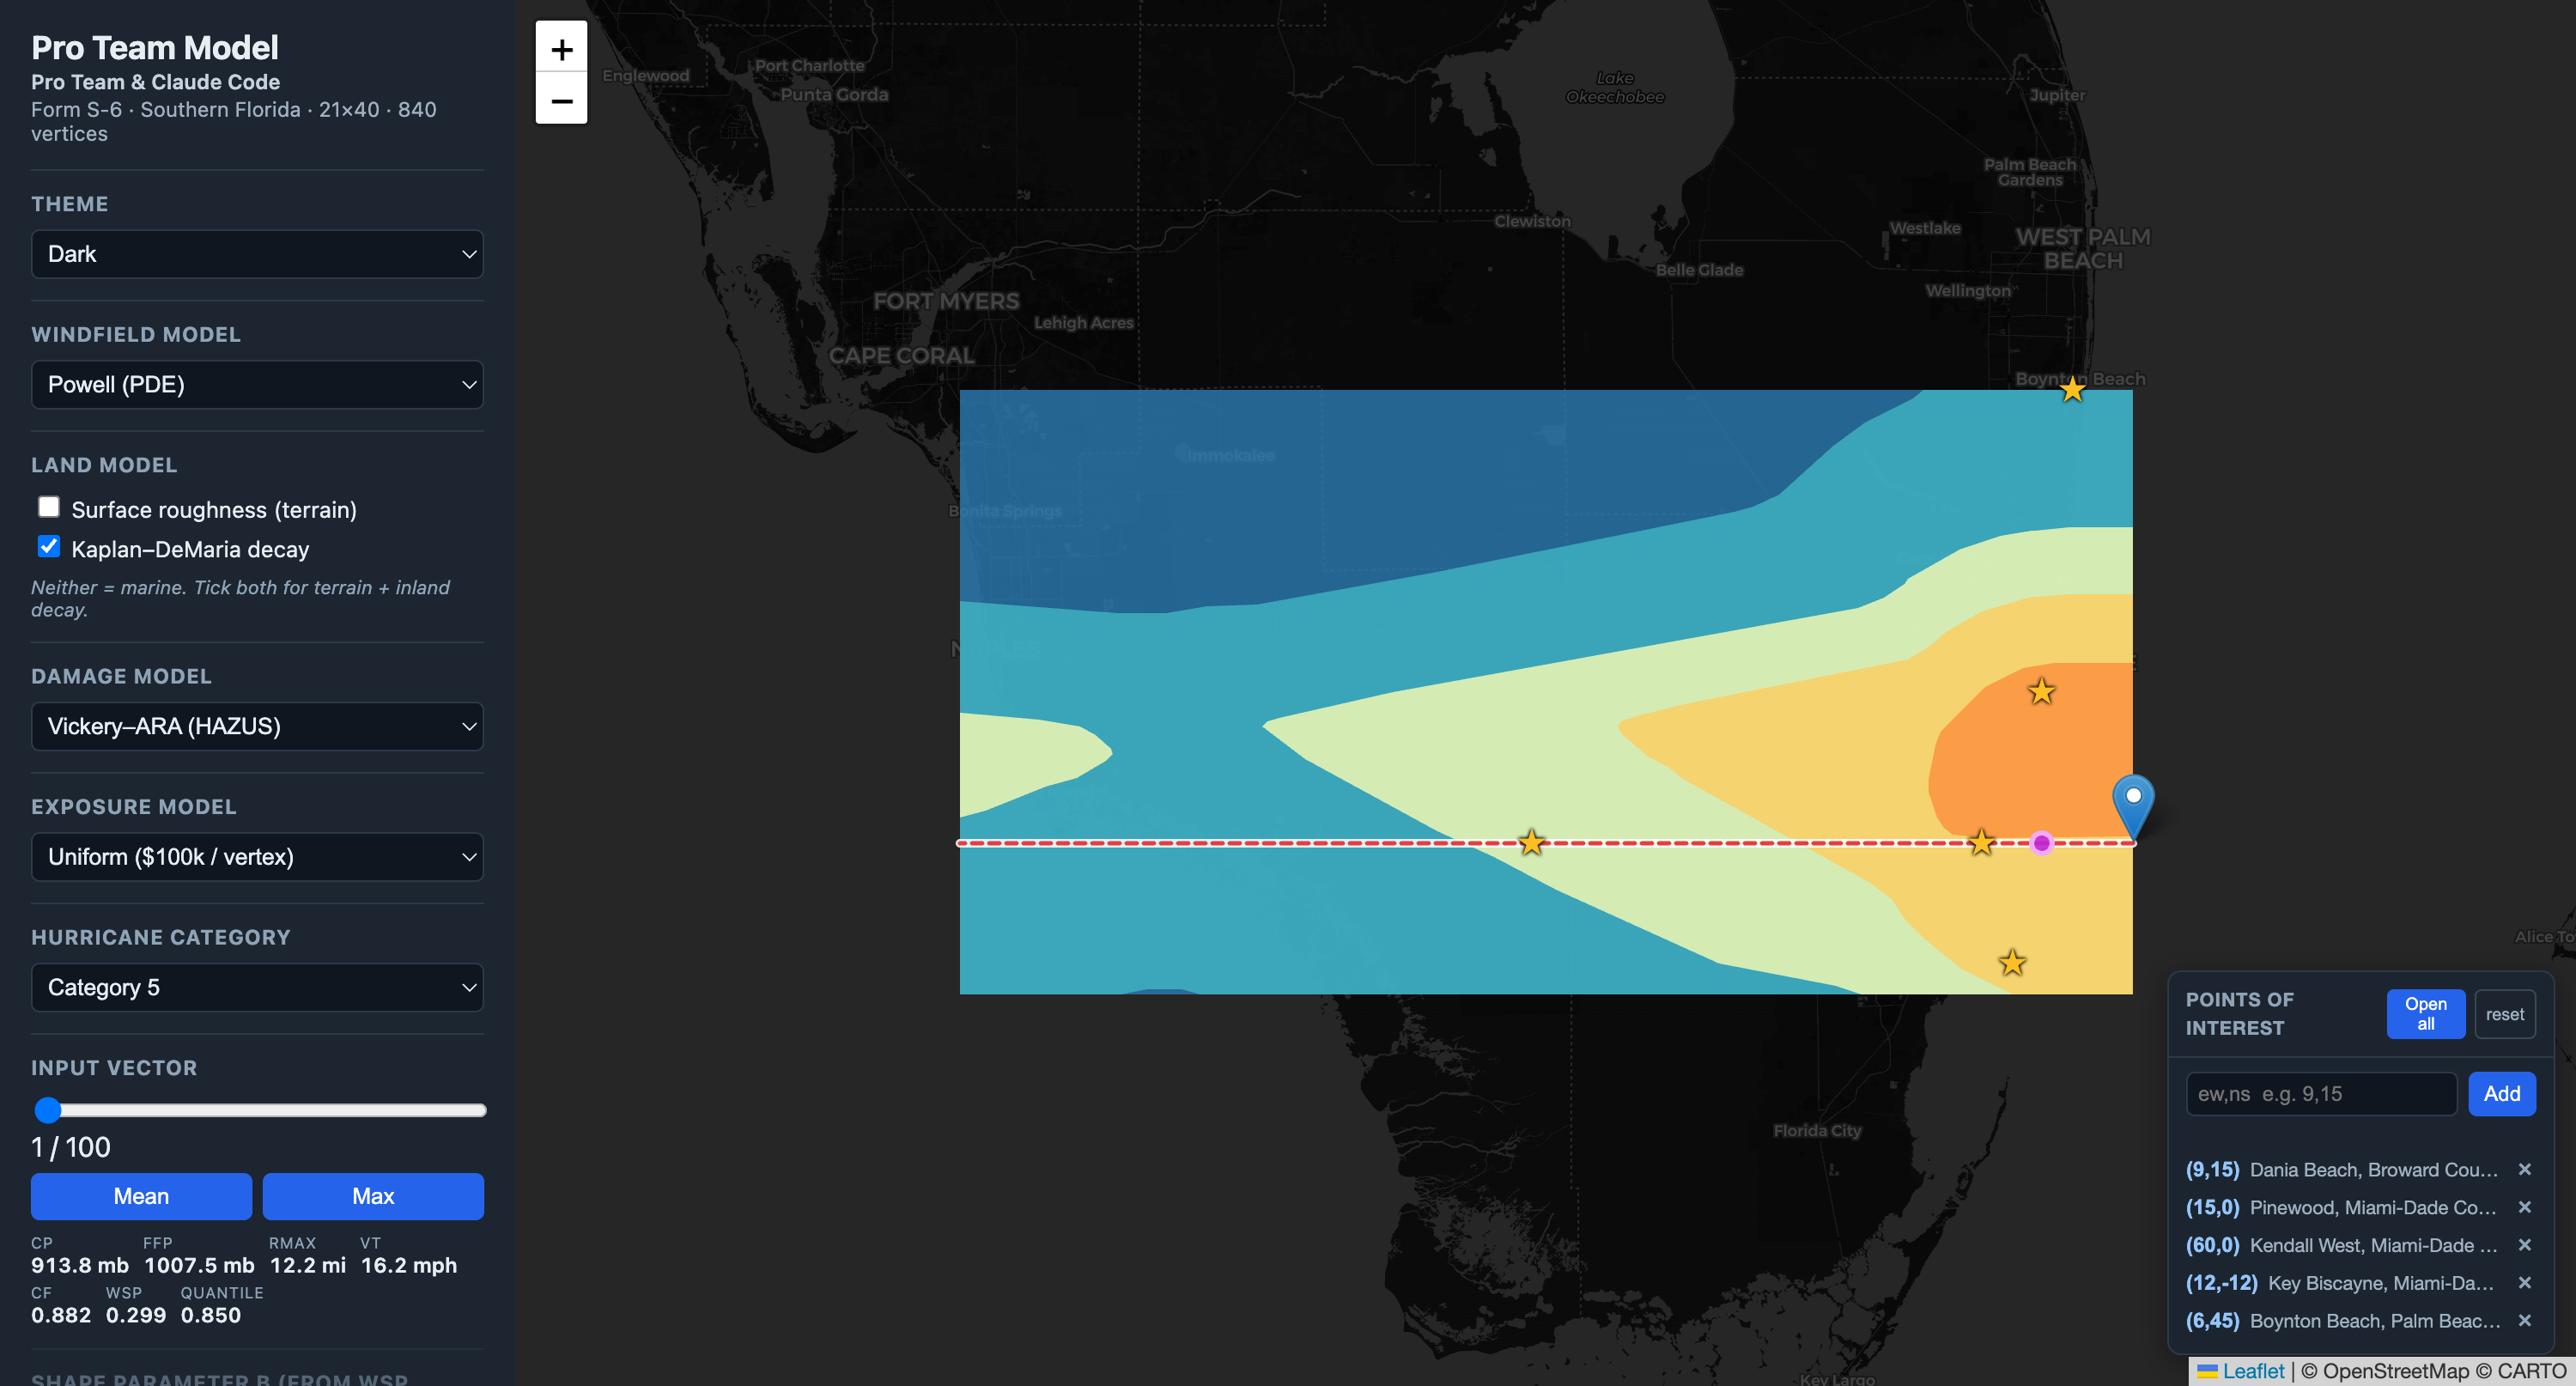
\includegraphics[width=0.49\textwidth]{powell_cat5_kd.png}\hfill
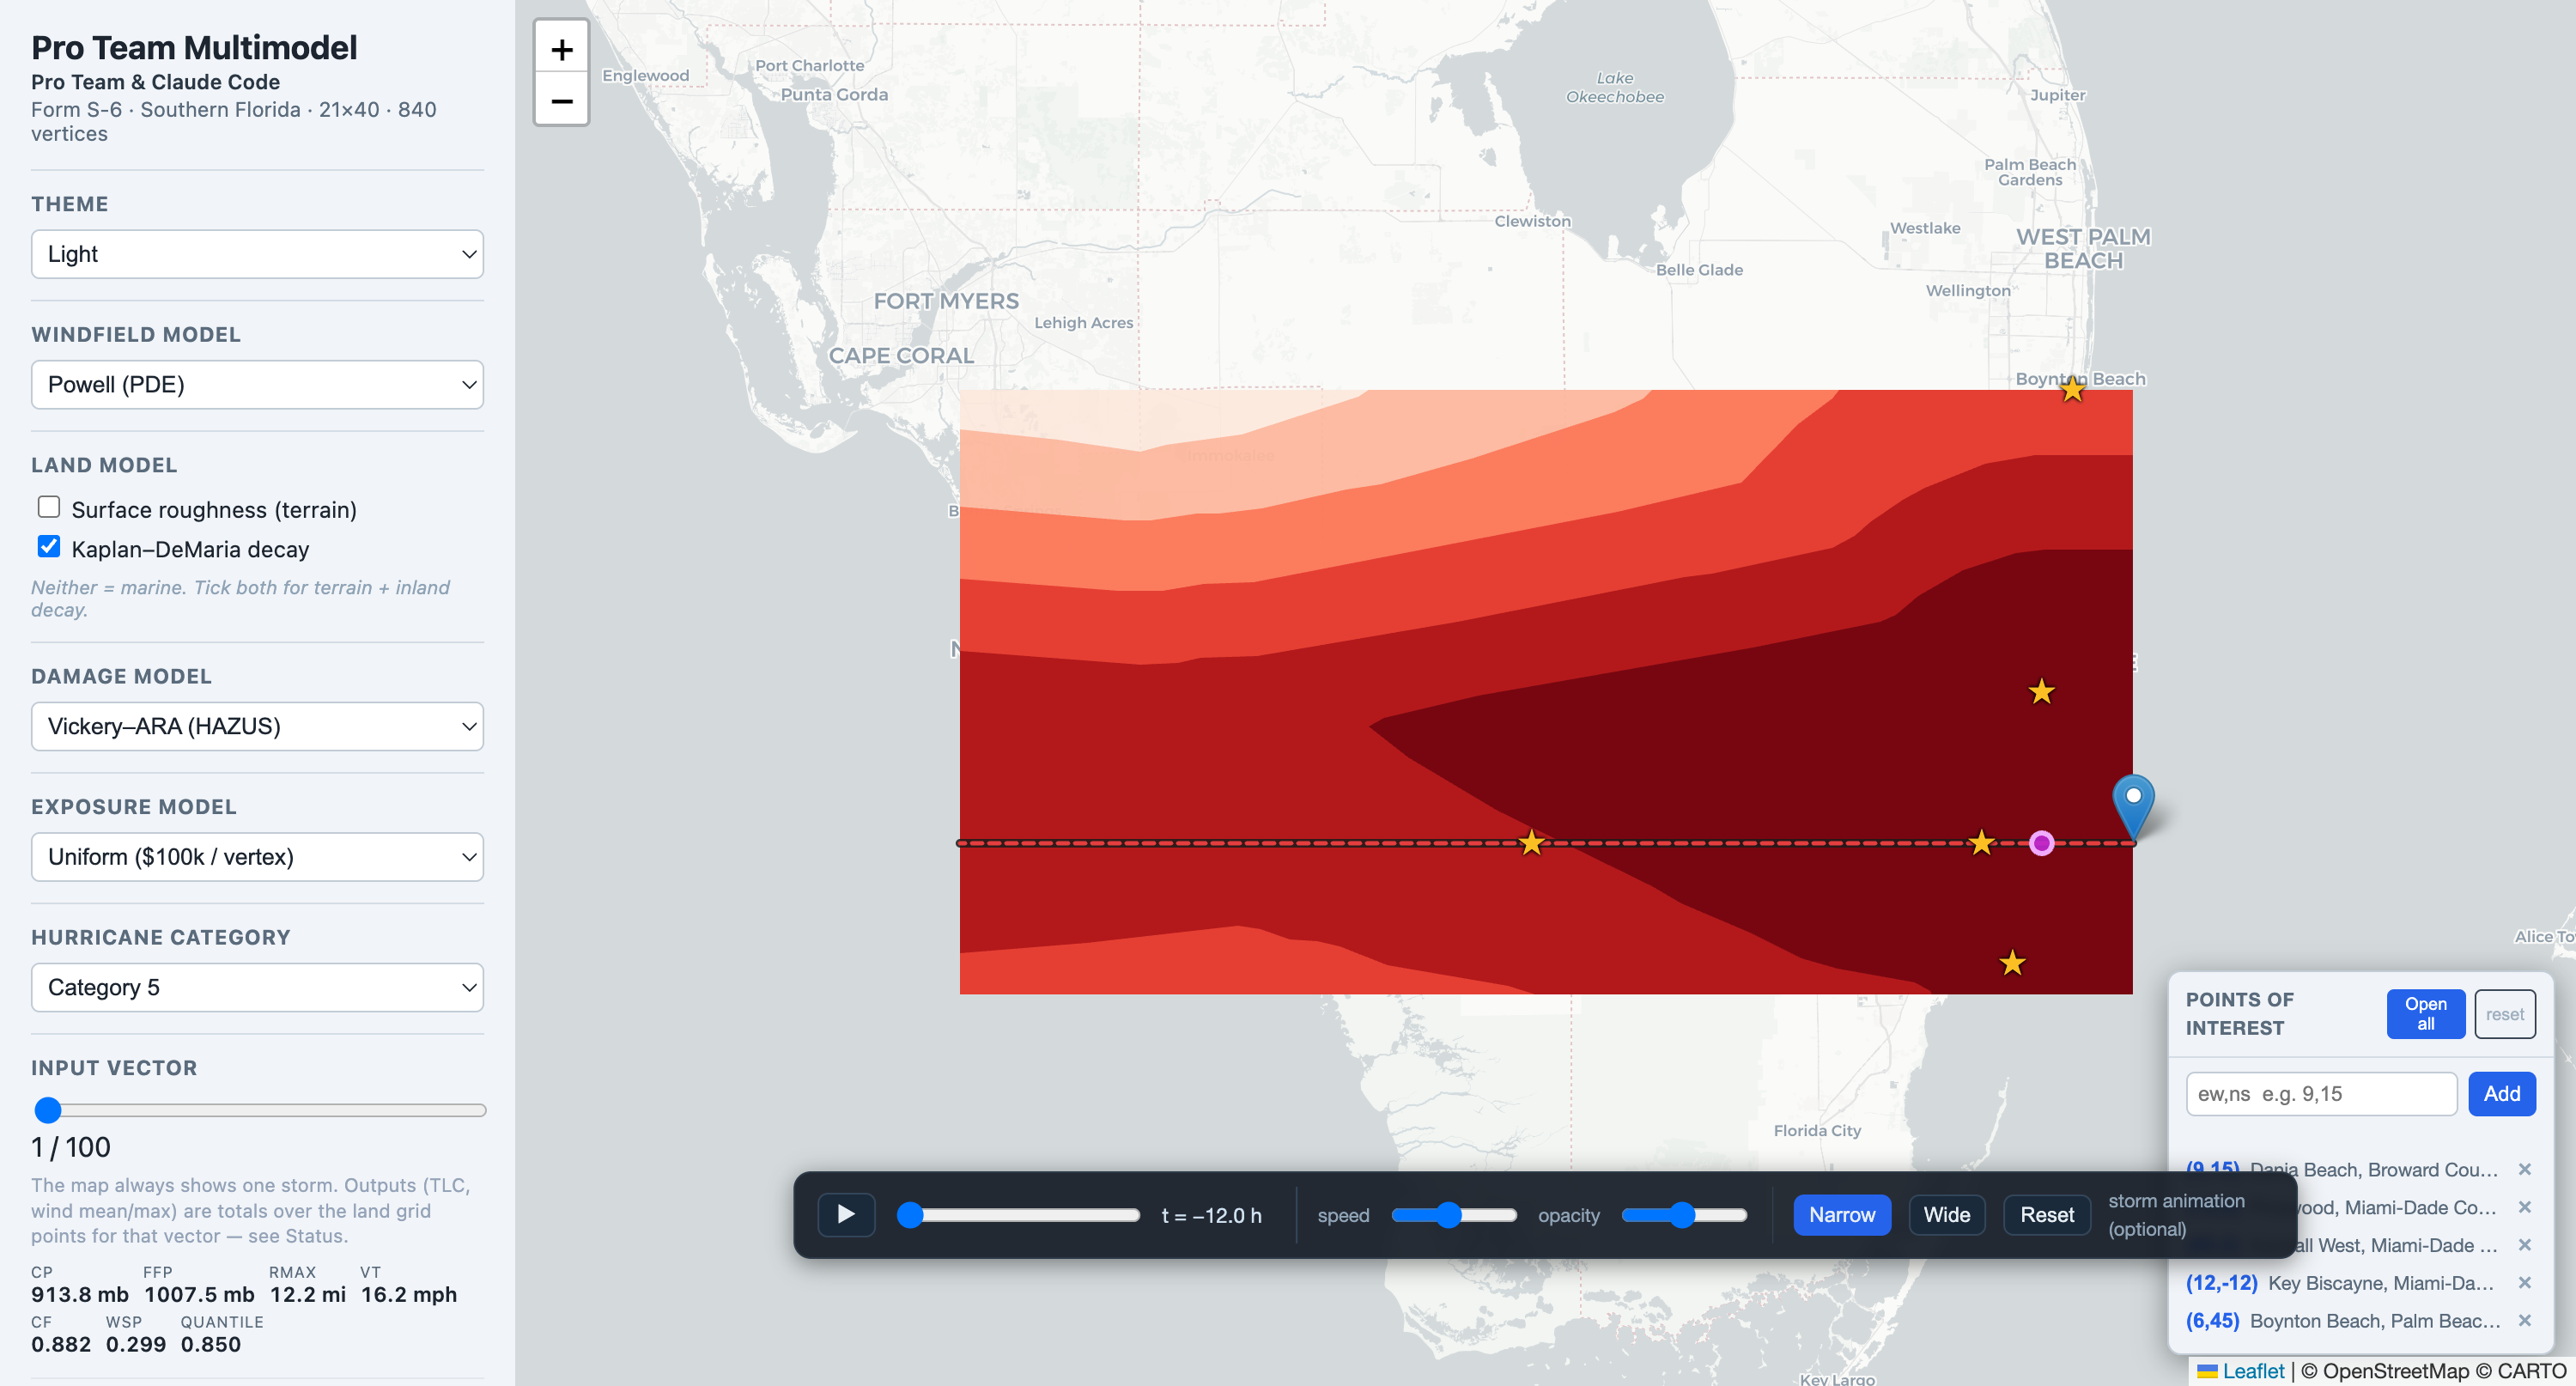
\includegraphics[width=0.49\textwidth]{powell_cat5_loss.png}
\caption{Category~5, Powell: Kaplan--DeMaria-decayed peak wind (left) and the
loss field as Mean Damage Ratio (right), both as filled contours.}
\label{fig:kdloss}
\end{figure}

\section{Statistics: Sensitivity and uncertainty analysis}\label{sec:sa}
Following Iman, Johnson, and Schroeder (2001)~\cite{iman}, as the ROA cites:
\begin{itemize}
\item \textbf{Sensitivity (SRC).} Standardized regression coefficients from
regressing the standardized output on the six standardized inputs over the 100
SA vectors, per category. Sign gives direction, magnitude gives influence
(ROA Fig.~9).
\item \textbf{Uncertainty (EPR).} Expected percentage reduction in output
variance per input (ROA Fig.~10). For \emph{Powell} the EPR is the variance share
\[
\text{EPR}_i=\frac{\mathrm{Var}\!\left(Y\,\middle|\,\text{only }X_i\text{ varies}\right)}
{\mathrm{Var}(Y_{\text{SA}})}\times100\%,
\]
computed faithfully from the six one-variable ROA ``UA for $X$'' worksheets
(1{,}800 PDE solves); the analytic models use the
$\text{EPR}_i=\text{SRC}_i^2$ approximation.
\end{itemize}
The output metric is the \textbf{mean peak wind over the 682 land vertices}
(loss-cost is the additional metric in Section~\ref{sec:loss}). The computed
SRCs and faithful EPRs reproduce the ROA's findings: WSP dominates for
Category~1 while Rmax grows to dominate for Category~5 (faithful EPR: Cat~1
WSP~$\approx54\%$, Cat~5 Rmax~$\approx57\%$), with CP negative and CF, FFP, Rmax
positive (Figure~\ref{fig:analysis}).

\begin{figure}[H]
\centering
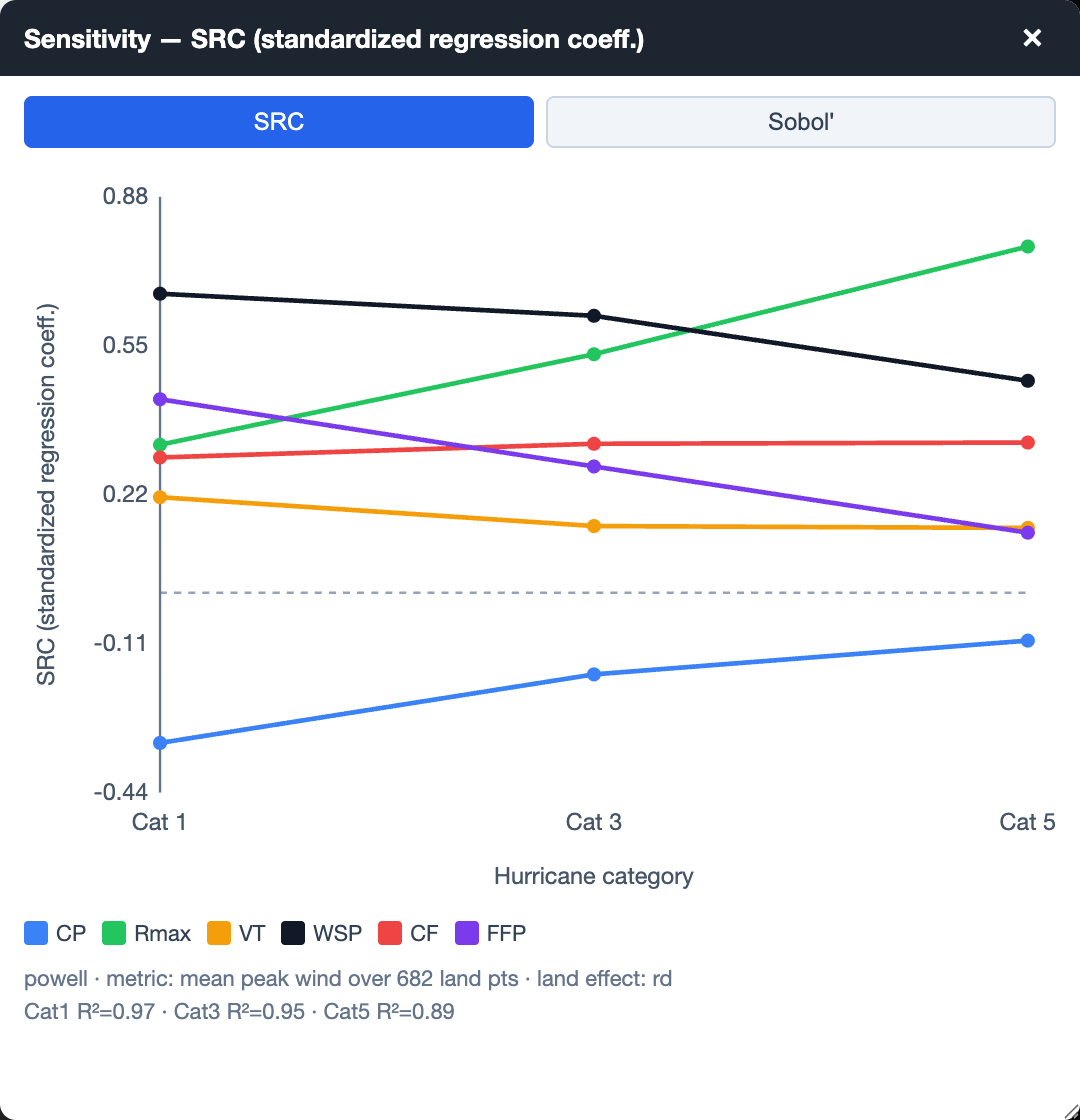
\includegraphics[width=0.49\textwidth]{analysis_src.png}\hfill
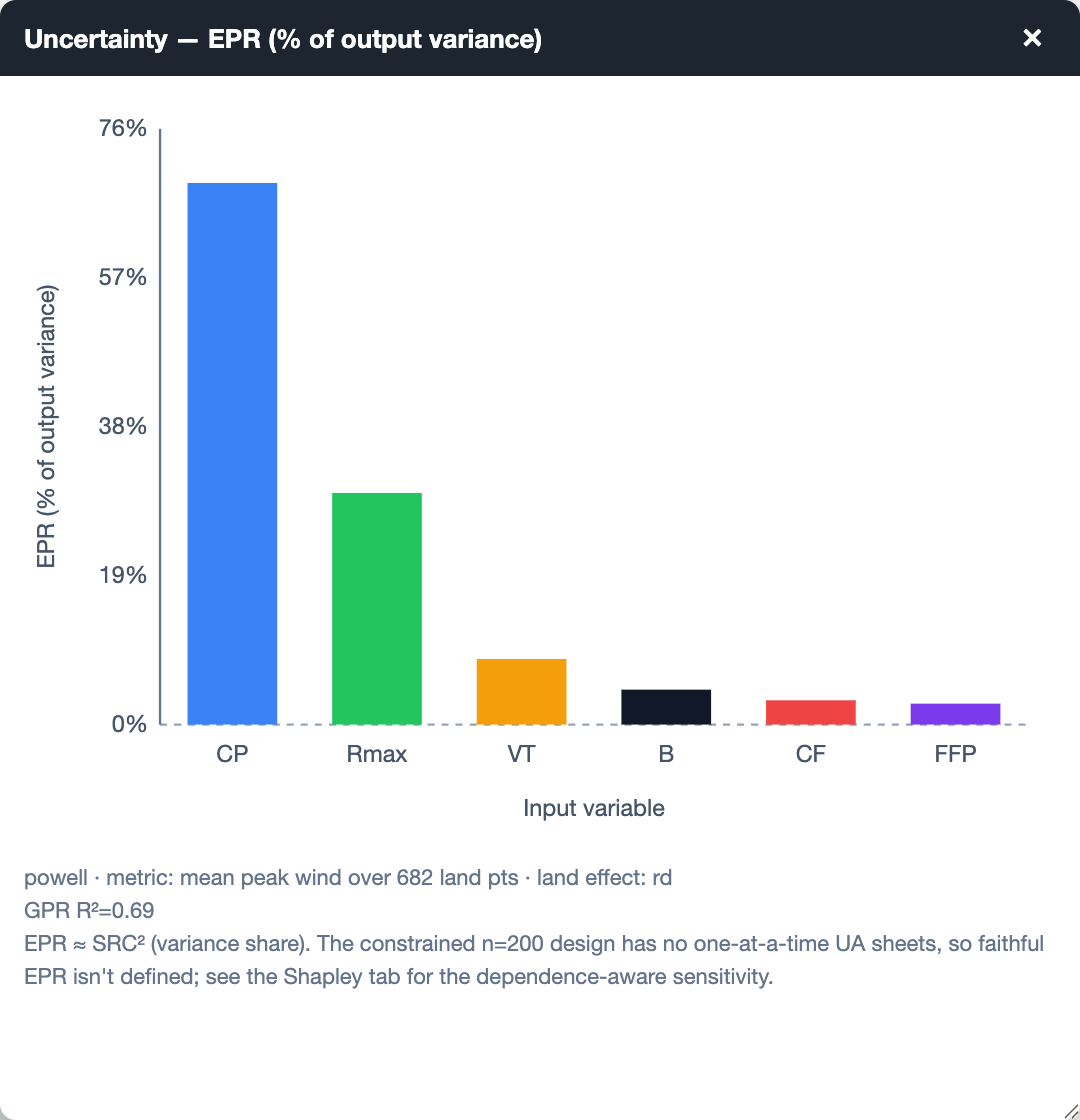
\includegraphics[width=0.49\textwidth]{analysis_epr.png}
\caption{Sensitivity (SRC, left) and uncertainty (EPR, right) for the Powell
model, plotted by hurricane category---the interactive analogues of ROA
Figs.~9--10. The windows are independently movable and resizable.}
\label{fig:analysis}
\end{figure}

\section{Statistics: Sobol' indices (variance-based SA)}\label{sec:sobol}
SRC is a \emph{first-order, linear} measure: it fits a plane through the response
and reports the slopes. If the response bends, or if two inputs act jointly, SRC
cannot see it. \textbf{Sobol' indices} \cite{sobol} answer the same question
(``how is output uncertainty apportioned among the inputs?'') without assuming
linearity, by decomposing the output \emph{variance} rather than fitting a line.
Following the functional ANOVA decomposition,
\[
\mathrm{Var}[f(\mathbf{x})]=\sum_i \mathrm{Var}[f_i(x_i)]
 +\sum_{i<j}\mathrm{Var}[f_{ij}(x_i,x_j)]+\cdots ,
\]
and dividing through by $\mathrm{Var}[f(\mathbf{x})]$ gives the \textbf{first-order}
index $S_i$ (the variance explained by input $i$ \emph{alone}) and the
\textbf{total} index $S_{T i}$ (input $i$ alone \emph{plus} every interaction it
participates in). The gap $S_{Ti}-S_i$ is therefore a direct, quantitative measure
of interaction---precisely the information SRC discards. Likewise
$\sum_i S_i < 1$ signals that the main effects do not account for the whole
variance, the shortfall being interaction.

\paragraph{Why an emulator is required.} Sobol' estimation is Monte-Carlo and needs
far more model evaluations than the $100$ Form S-6 vectors provide. The standard
remedy, and the one recommended in the practitioner review of Francom and
Nachtsheim \cite{francom}, is to fit an \emph{emulator} to the available runs and
compute the indices on \emph{it}. We do exactly that: the indices are evaluated on
the Gaussian-process metamodel of Section~\ref{sec:metamodel}, using the Saltelli
\cite{saltelli2010} estimator for $S_i$ and the Jansen \cite{jansen1999} estimator
for $S_{Ti}$, at $n=262{,}144$ samples averaged over three independent replicates.
A separate emulator is fit for \emph{each land configuration}---surface roughness
alone, and roughness with Kaplan--DeMaria decay---so the reported indices always
describe the configuration actually selected in the viewer. Decay makes the response
\emph{more} interactive, as one would expect of an added nonlinear process: for
Cat~1 loss cost, $\sum_i S_i$ falls from $0.90$ to $0.83$ when it is switched on.

\paragraph{Assumptions, checked.} Sobol' requires \emph{independent} inputs and an
explicit input distribution. Both were verified rather than assumed. The six inputs
are effectively uncorrelated (largest $|r|$ across the $15$ pairs is $0.04$ for
Cat~1 and $0.05$ for Cat~3; Cat~5 shows a mild $r=+0.29$ between CP and $R_{\max}$,
about $2.9\sigma$ at $n=100$ and consistent with Latin-hypercube sampling noise).
Their marginals are \emph{uniform} over the sampled ranges (Kolmogorov--Smirnov
$p=0.11$, $0.06$, $0.16$, and $1.00$ for CP, $R_{\max}$, VT, and WSP/CF/FFP), so
sampling the Sobol' design uniformly on the observed box is the correct reference
measure. A convergence check was also necessary: at the naive $n=2048$ the
estimates still drifted by $\sim$$0.05$---as large as the interaction effect they
were meant to detect---so the sample size was raised until the Monte-Carlo error
fell an order of magnitude below the signal.

\paragraph{Result: the model is nearly additive, with one real interaction.}
Across all three categories and both responses, $\sum_i S_i$ lands between $0.90$
and $0.97$: the main effects alone explain $90$--$97\%$ of the output variance, so
the response is \emph{mostly} additive and SRC is not badly wrong. But the
remaining $3$--$10\%$ is genuine interaction, and it is not spread evenly. The gap
$S_{Ti}-S_i$ is significant (above its Monte-Carlo error) for $R_{\max}$ and WSP,
and the second-order indices localise it precisely: $S_{ij}$ for the
$R_{\max}\times$WSP pair is $+0.02$ to $+0.05$, an order of magnitude larger than
any other pair, which sit at $\approx 0$. The storm's size and its wind-profile
shape act on the loss \emph{jointly}---which is exactly what the interaction matrix
(Figure~\ref{fig:matrix}) shows by eye, and what a linear SRC cannot express.

\begin{figure}[H]
\centering
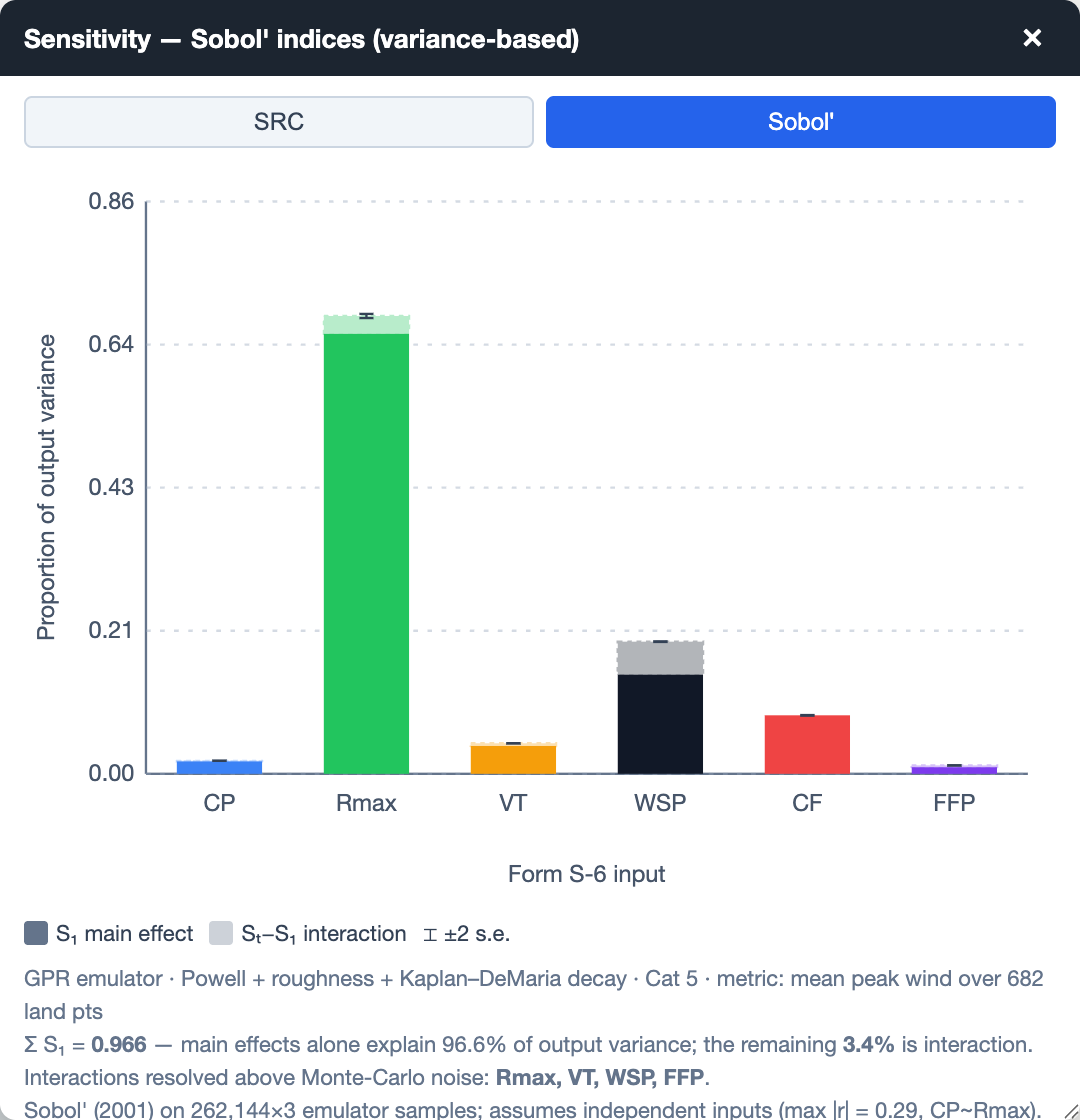
\includegraphics[width=0.62\textwidth]{analysis_sobol.png}
\caption{Sobol' indices for Cat~5 peak wind, computed on the GPR emulator. Each bar
is an input: the solid part is the main effect $S_i$, the shaded cap is the
interaction $S_{Ti}-S_i$, and the whisker is $\pm2$ Monte-Carlo standard errors.
$R_{\max}$ dominates; WSP carries the largest interaction share. The panel is
reached from \textbf{Sensitivity} via the SRC\,/\,Sobol' method tabs, so the two
methods sit one click apart.}
\label{fig:sobol}
\end{figure}

\section{Statistics: Metamodels and the interaction profiler}\label{sec:metamodel}
The standardized regression coefficients of Section~\ref{sec:sa} treat the
input--output map as \emph{first order}: each input acts independently and
linearly. The Sobol' analysis of Section~\ref{sec:sobol} shows this is not quite
true---$3$--$10\%$ of the output variance is interaction, concentrated in the
$R_{\max}\times$WSP pair---which motivates replacing the linear fit with a flexible
\emph{metamodel} (response surface, Gaussian-process regression, or neural
network) examined through an interaction \emph{profiler}. The viewer implements
this directly.

\paragraph{Response variable.}
A \textbf{Response (Y)} selector chooses the scalar output that every analysis
tool regresses on. Every choice is an aggregate over the 682 land \emph{grid
points} of a \emph{single} input vector---never an average across vectors---and the
selector is therefore also the control for \emph{which} grid-point statistic is
reported: the \textbf{mean peak wind} (the domain-average storm), the \textbf{max
peak wind} (the worst-hit vertex), or the \textbf{loss cost} $\%\text{TLC}(i)$ (the
domain total), defined exactly as in Section~\ref{sec:loss},
\[
\%\text{TLC}(i)=\frac{\text{TLC}(i)}{\$68{,}200{,}000}\times100\%
=100\times\overline{\text{MDR}}_{\text{land}}(i),
\]
the total loss cost of input vector $i$ as a percent of total exposure, equal to
$100\times$ the mean Mean-Damage-Ratio over the 682 land vertices. Switching the
response re-fits the SRC, EPR, profiler, and CDF panels live (for loss-cost the
faithful EPR worksheets do not apply, so the $\text{SRC}^2$ variance share is
used). Two further responses---\emph{duration} and \emph{wind dosage}---are
location-level diagnostics available only in single-point mode; they are defined
with the spatial-scale toggle below.

\paragraph{The aggregate is not a cosmetic choice.} Which grid-point statistic one
takes \emph{changes which input dominates}. For Category~5 (roughness and decay on)
the first-order Sobol' indices are
\[
\begin{array}{lccc}
\text{input} & \text{mean wind} & \text{max wind} & \%\text{TLC}\\\hline
R_{\max} & \mathbf{0.659} & 0.066 & \mathbf{0.469}\\
\text{WSP} & 0.149 & \mathbf{0.748} & 0.314\\
\text{VT} & 0.042 & 0.000 & 0.040
\end{array}
\]
Storm \emph{size} ($R_{\max}$) governs the domain mean and the total loss---it sets
how much of the grid is struck at all. But the \emph{profile shape} (WSP, hence $B$)
governs the worst-hit vertex, because it sets the eyewall peak; there $R_{\max}$
collapses to $0.07$ and forward speed to zero. A sensitivity ranking is therefore
only meaningful once the output has been named, which is precisely the
statistician's point: the quantity of interest is an aggregate over the grid points
of a \emph{given} vector, and different aggregates are different questions.

\paragraph{Second-order metamodel.}
For the profiler the viewer fits, per category, a standardized second-order
response surface in the six inputs $z_k=(X_k-\bar X_k)/s_{X_k}$,
\[
\hat Y=b_0+\sum_{k} b_k z_k+\sum_{k} b_{kk} z_k^{2}
        +\sum_{j<k} b_{jk}\,z_j z_k ,
\]
i.e.\ linear, quadratic, and all $15$ pairwise cross terms ($28$ coefficients,
fit by least squares over the $100$ Latin-hypercube vectors via the normal
equations with a small ridge for stability). The quadratic and cross terms are
what let the metamodel \emph{bend} and express interactions; a purely linear fit
would draw flat, parallel profiles. Because the simulator is a smooth
deterministic function of the six inputs, this surface typically reproduces the
$100$ runs almost exactly ($R^2\!\approx\!1$).

\paragraph{Interaction profiler.}
The profiler (Figure~\ref{fig:profiler}) draws one partial-dependence curve per
input: $\hat Y$ as that input sweeps its range while the other five are held at a
reference point shown by the dashed crosshair. Six sliders set the reference
point (initialized at the input means). Dragging one slider re-draws the other
five curves; \emph{a curve whose slope changes is interacting with the moved
variable}. This is the JMP-style ``prediction profiler'' of the review deck: for
the Category-5 Powell fit, for example, the $R_{\max}$ profile is strongly
concave and its slope steepens as CP is lowered (more intense storms), the
signature two-factor CP\,$\times$\,$R_{\max}$ interaction.

\begin{figure}[H]
\centering
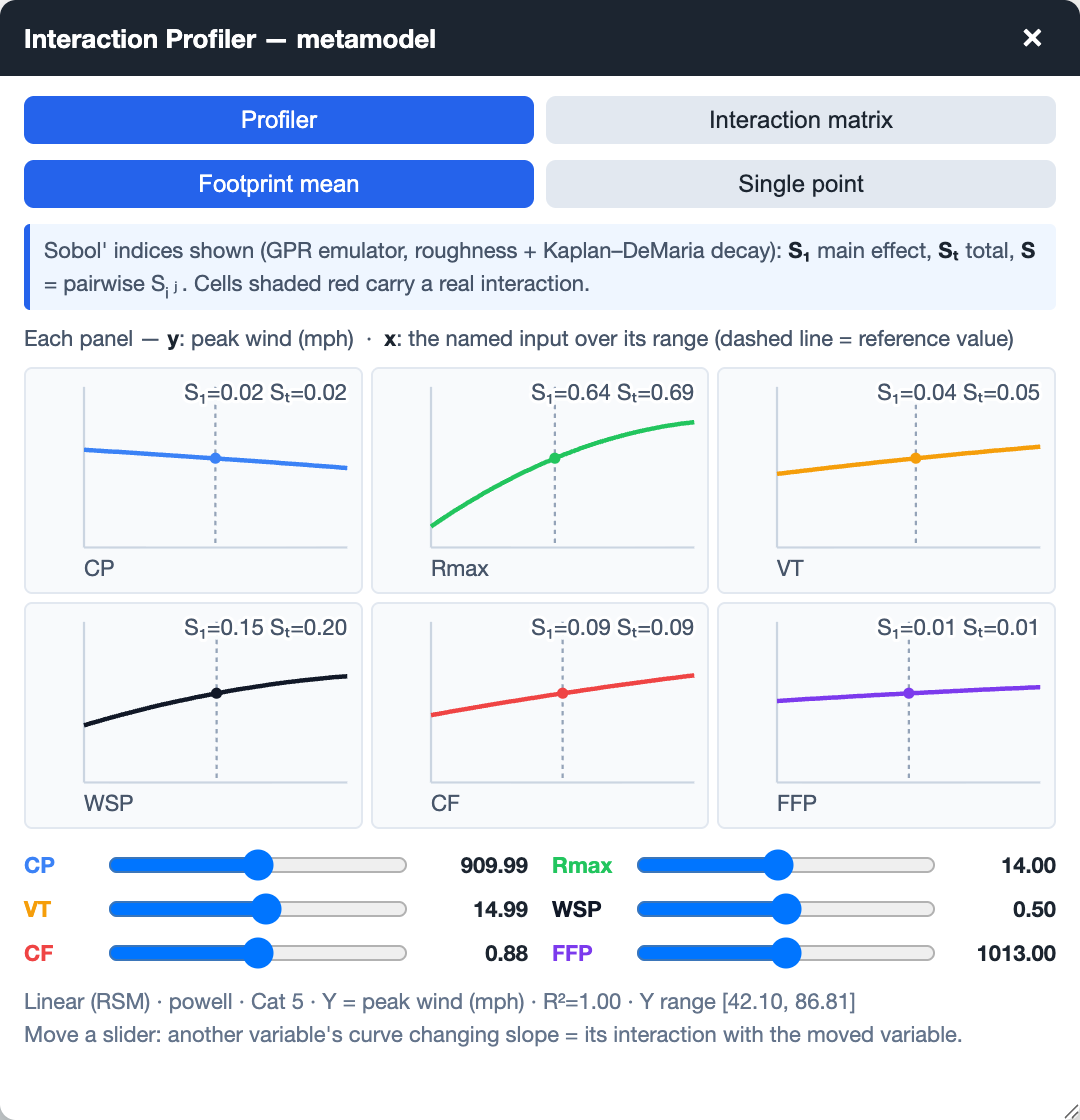
\includegraphics[width=0.7\textwidth]{analysis_profiler.png}
\caption{Interaction profiler for the Category~5 Powell metamodel
($Y=$ mean peak wind). Each panel is the partial-dependence of $\hat Y$ on one
input with the others held at the slider reference point (dashed crosshair).
Moving a slider re-renders the other curves, so a change of slope reveals the
interaction between that pair of variables.}
\label{fig:profiler}
\end{figure}

\paragraph{Interaction matrix.}
A \textbf{Profiler\,$\,\leftrightarrow\,$Interaction matrix} toggle at the top of the
panel offers a second, all-at-once view of the same metamodel
(Figure~\ref{fig:matrix}). It is an $N\!\times\!N$ grid over the six inputs: the
diagonal labels each variable with its min$\,\to\,$max range, and each off-diagonal
cell $(r,c)$ draws the effect of input $c$ on $\hat Y$ with input $r$ held at its
\textcolor{blue}{minimum (blue)} and \textcolor{red}{maximum (red)}, all other
inputs at their mean---a temperature metaphor, so red always reads as the high end
of a scale. Parallel blue and red curves mean no interaction; diverging
slopes or a widening gap mean $r$ and $c$ interact. Where the slider profiler is the
interactive explorer (one reference point at a time), the matrix is a standing map
of \emph{every} pairwise interaction at once. Both views are driven by the same fit;
switching the \textbf{Metamodel} (Linear/GPR/NN) or response redraws either.

Each off-diagonal cell is also \emph{annotated with its second-order Sobol' index}
$S_{ij}$ (Section~\ref{sec:sobol}) and shaded in proportion to it, which turns a
qualitative ``do these curves diverge?'' judgement into a measured one. The effect is
striking: only the $R_{\max}\times$WSP cells shade red ($S_{ij}=0.055$), while every
other pair reads $S_{ij}\approx 0.000$ and draws visibly parallel curves. A viewer
might otherwise over-read a small visual separation elsewhere; the index says it is
noise. The profiler likewise labels each input's panel with its $S_i$ and $S_{Ti}$,
pairing the \emph{shape} of an effect with its \emph{magnitude}.

\begin{figure}[H]
\centering
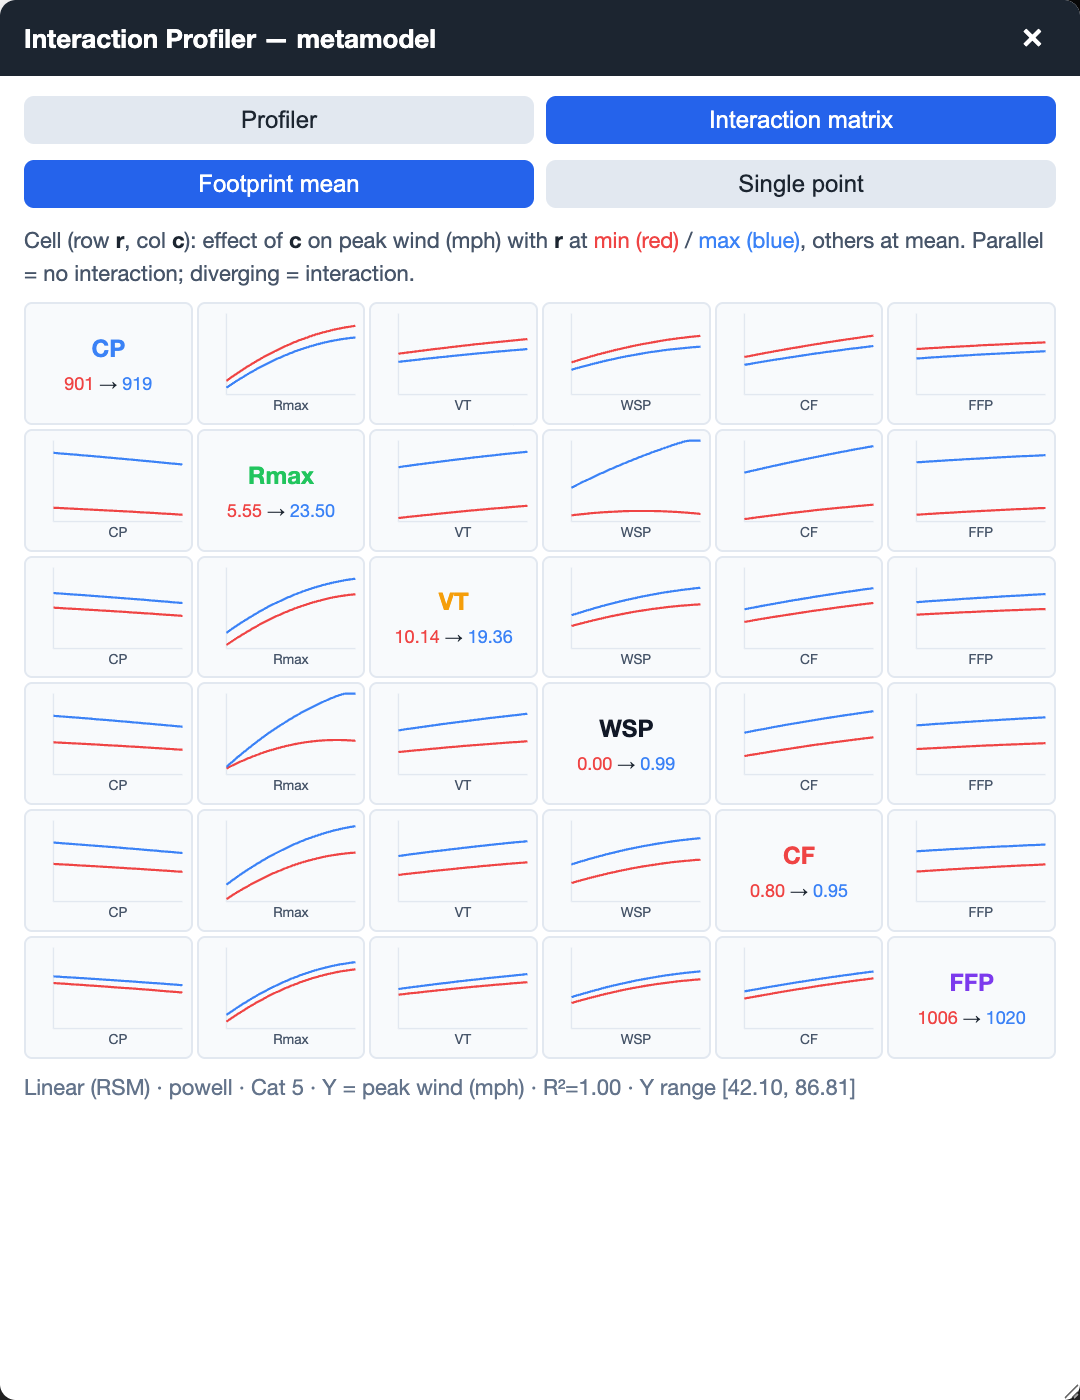
\includegraphics[width=0.82\textwidth]{analysis_matrix.png}
\caption{Interaction-matrix view (Category~5 Powell, $Y=$ mean peak wind). Diagonal:
each input and its min$\to$max range. Off-diagonal cell $(r,c)$: the effect of input
$c$ with input $r$ at \textcolor{blue}{min (blue)} vs \textcolor{red}{max (red)},
others at their mean; diverging curves indicate an $r\times c$ interaction. Each cell
is annotated with its second-order Sobol' index $S_{ij}$ and shaded by it---only
$R_{\max}\times$WSP lights up.}
\label{fig:matrix}
\end{figure}

\paragraph{Single point vs.\ footprint (spatial scale).}
A second toggle, \textbf{Footprint mean\,$\,\leftrightarrow\,$Single point}, changes the
spatial scale of the response and exposes a subtle but important effect. In
\emph{footprint} mode the response is the $682$-vertex mean (the metamodel above). In
\emph{single point} mode the user clicks a grid vertex on the map and the curves are
recomputed by \emph{direct wind-field simulation} at that one location---peak wind
there, optionally through the damage curve for $\%\text{LC}$---rather than a metamodel,
because a quadratic surface cannot represent the inflection that appears point-wise.
The contrast is instructive: the loss-vs-$R_{\max}$ response at a single off-track
vertex is a clean \textbf{S} (Figure~\ref{fig:matrixpt}), as the growing eyewall sweeps
the point through the steep middle of the damage sigmoid, whereas the footprint mean is
\emph{concave}---averaging $682$ vertices, each crossing that sigmoid at a different
$R_{\max}$, smooths the S into a saturating ramp ($517$ of the $682$ land points are
individually S-shaped). Spatial resolution thus changes both the shape of the loss
response and the apparent strength of its interactions---a concrete cautionary lesson
for catastrophe-model interpretation. For \textbf{Holland/Willoughby} single-point
mode runs this \emph{direct simulation} at the vertex, applying surface roughness
and/or Kaplan--DeMaria decay live (whichever land toggles are set) so it stays
consistent with the footprint---the live decayed peak matches the precomputed decayed
field to within $\sim$0.02\,mph. \textbf{Powell} has no closed-form field to
re-simulate, so its single-point sensitivity instead fits a \emph{per-vertex
second-order response surface} live from the 100 precomputed peaks at the picked
vertex (the same 100-vector data the grid-sensitivity map uses, honouring roughness
and decay through the stored field), and the profiler sweeps the inputs through it;
this covers peak wind and \%LC (the duration metrics, which need a time series, remain
live-model only). The panel labels which is in use---``direct simulation'' vs
``per-vertex RSM''.

\begin{figure}[H]
\centering
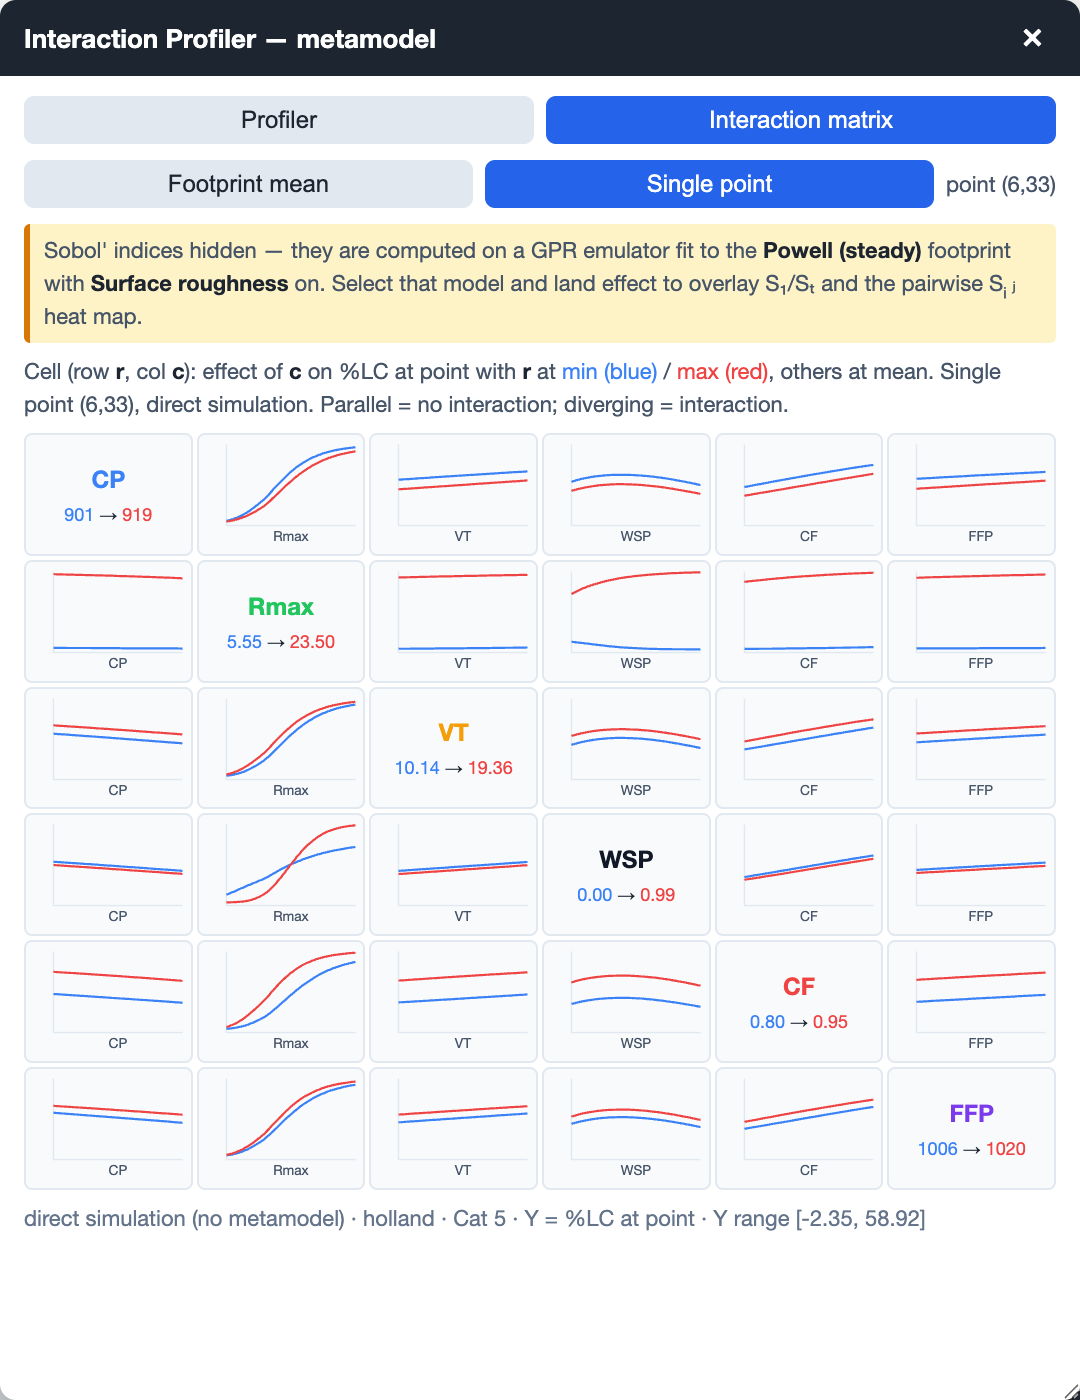
\includegraphics[width=0.82\textwidth]{analysis_matrix_point.png}
\caption{Single-point interaction matrix (Holland, Category~5, vertex $(6,33)$ Boca
Raton, $Y=\%\text{LC}$ at the point, direct simulation). The $R_{\max}$ column is
visibly \textbf{S-shaped}---contrast the concave footprint-mean version in
Figure~\ref{fig:matrix}. The sigmoid that survives at a single location averages out
over the full footprint.}
\label{fig:matrixpt}
\end{figure}

\paragraph{Duration of exposure (location-level loss).}
Damage accumulates for as long as the wind stays above the threshold at which it
begins ($\sim$40\,mph), so the \emph{peak} wind at a location is an incomplete
predictor of loss: a slow or large storm holds a point above threshold much longer
than a fast, compact one of the same peak, yet the peak-driven MDR---and the
published HAZUS curve (Section~\ref{sec:vuln})---score them identically. To make
this visible at the location level, the Response selector offers two
duration-of-exposure diagnostics computed by the same direct single-point
simulation from the per-point wind time series $V(t)$ over the passage,
\[
\text{dwell}=\!\!\int_{V(t)\ge V_0}\!\!\!\! dt \ \ (\text{h}),
\qquad
\text{dosage}=\!\!\int \big(V(t)-V_0\big)_{+}\, dt \ \ (\text{mph}{\cdot}\text{h}),
\qquad V_0=40\,\text{mph},
\]
where dwell counts the hours the wind exceeds the threshold and dosage weights each
hour by how far it exceeds it (the excess-wind ``area'' the storm deposits). Both
are profiled and matrixed exactly like the peak/\%LC responses. The sensitivity the
peak metric hides is then explicit: at vertex $(6,33)$ the dwell falls from
$\approx11.6$ to $\approx6.8$\,h and the dosage from $\approx230$ to
$\approx150$\,mph$\cdot$h as the forward speed $V_T$ sweeps its range---a
first-order dependence on translation speed that the peak-wind response registers
as almost flat. These diagnostics are single-point only: the footprint stores hold
precomputed peak wind per vertex with no time series to integrate, so at footprint
scale (and in the SRC, EPR, and metamodel-comparison panels) they show a short
``location-level'' note.

\paragraph{Integrated Kinetic Energy (IKE) at a grid cell.}
A third review comment proposed Integrated Kinetic Energy as the natural integrated
hazard to tie to location-level loss. The Powell--Reinhold \cite{powellreinhold2007}
IKE is a \emph{spatial} integral of the surface kinetic-energy density
$\tfrac12\rho V^2$ over the area where $V\ge$ tropical-storm force ($\approx$34\,kt),
in a 1-m surface layer, reported for the whole storm in terajoules. Here we adapt it
to a \emph{temporal} integral at one fixed cell: a $1$-m-deep column over the
3\,mi\,$\times$\,3\,mi cell ($A\!\approx\!2.33\times10^7$\,m$^2$) holds instantaneous
energy $E(t)=\tfrac12\rho V(t)^2 A\,h$ whenever $V\ge V_0=40$\,mph, and we accumulate
it over the passage from the same per-cell time series $V(t)$ used above. Two
responses are exposed:
\[
\text{IKE}_{\text{int}}=\!\!\int_{V\ge V_0}\!\!\!\! E(t)\,dt \ \ (\text{TJ}{\cdot}\text{h}),
\qquad
\text{IKE}_{\text{peak}}=\max_{V\ge V_0} E(t) \ \ (\text{TJ}).
\]
The dimensions differ deliberately: the time-integrated energy is
terajoule-\emph{hours} (an accumulated exposure, the meteorologist's ``summed every
timestep'' quantity), while the peak is a snapshot in terajoules. For a single cell
the values run $\sim$$0.01$--$0.1$\,TJ$\cdot$h and $\sim$$0.01$--$0.05$\,TJ---a small
slice of the $10$--$200$\,TJ whole-storm IKE. As an integrated quantity, $\text{IKE}_
{\text{int}}$ behaves like the wind dosage (it falls as forward speed $V_T$ rises and
grows with intensity), but weights the wind quadratically ($\tfrac12\rho V^2$) with
physical energy units. A companion map colouring paints every land cell by
$\text{IKE}_{\text{int}}$ for a \emph{single} chosen storm (682 per-cell time series),
revealing where the storm deposits the most energy (Figure~\ref{fig:ikemap}), with
roughness and/or Kaplan--DeMaria decay applied. All three models are supported:
Holland/Willoughby build the series live, and Powell samples its stored
storm-relative field (as the left-click pop-up does)---so the map works even though
Powell has no closed-form field. The single-point IKE \emph{sensitivity} (the
profiler sweeping arbitrary parameters) remains live-model only, since Powell's
stored fields exist only at the 100 sampled vectors.

\begin{figure}[H]
\centering
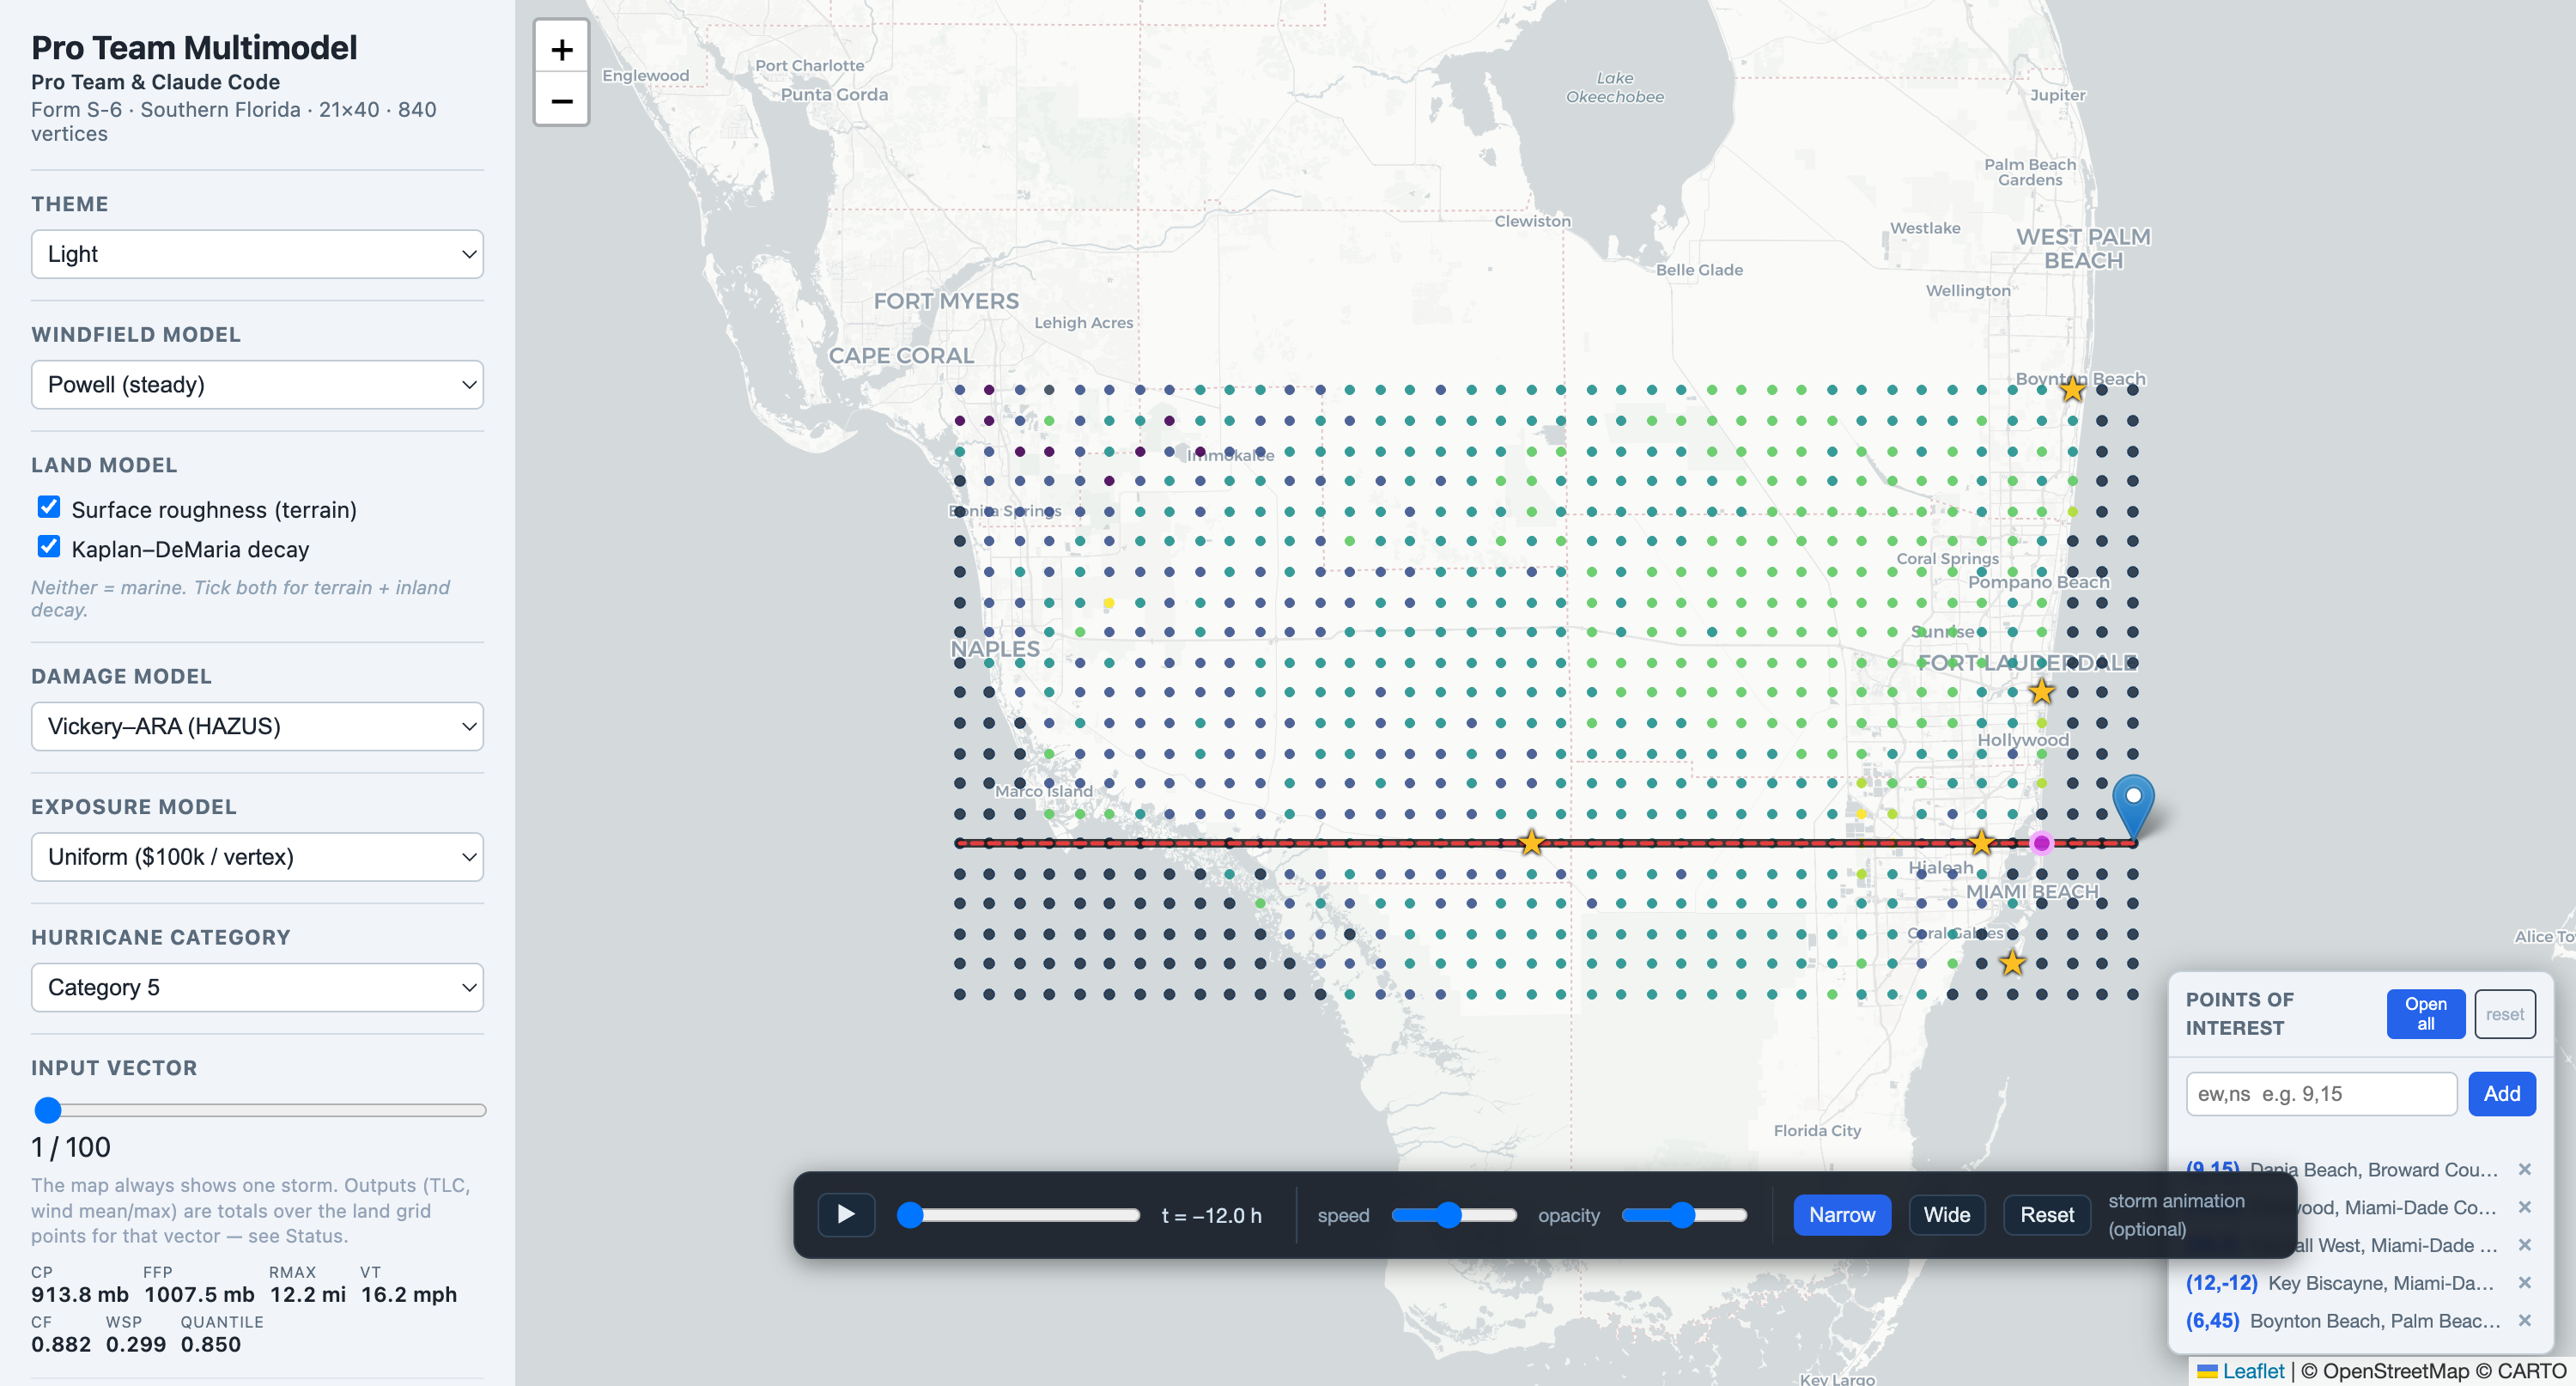
\includegraphics[width=0.82\textwidth]{ike_map.png}
\caption{Per-cell Integrated Kinetic Energy (IKE$_{\text{int}}$, TJ$\cdot$h) for a
single Category~5 Holland storm, accumulated while $V\ge40$\,mph. Brighter (viridis
yellow) cells accumulate more energy---concentrated along the track band where the
strong winds dwell---fading to dark toward the off-track edges; cell-to-cell speckle
reflects terrain roughness modulating the surface wind.}
\label{fig:ikemap}
\end{figure}

\paragraph{Loss-cost distribution.}
A companion panel plots the empirical CDF of $\%\text{TLC}(i)$ over the $100$
vectors for the selected category (the ROA's Fig.~5 analogue), summarizing the
spread of simulated loss cost. For Category~5 (Figure~\ref{fig:tlccdf}) the loss
cost ranges from roughly $14\%$ to $53\%$ of exposure with a mean near $33\%$.

\begin{figure}[H]
\centering
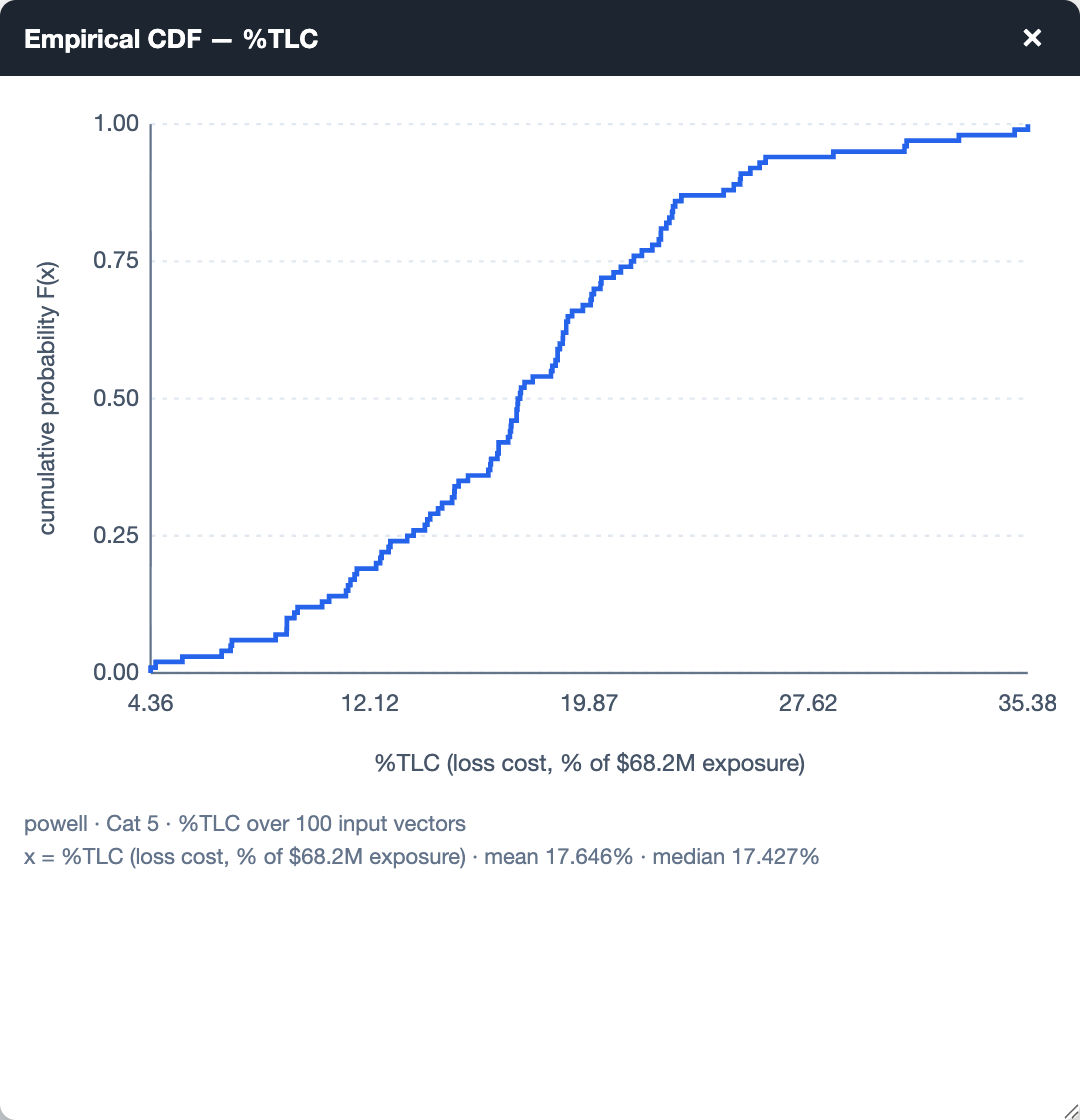
\includegraphics[width=0.62\textwidth]{analysis_tlc_cdf.png}
\caption{Empirical CDF of $\%\text{TLC}(i)$---loss cost as a percent of the
\$68.2M exposure---over the $100$ Category~5 input vectors (Powell).}
\label{fig:tlccdf}
\end{figure}

\paragraph{Loss exceedance and financial metrics (actuarial layer).}
The viewer adds the third catastrophe-model leg---the financial module---on top of
the hazard (wind field) and vulnerability (MDR) chain, grouping the analysis tools
into \textbf{Statistics} (sensitivity, uncertainty, profiler, metamodel comparison)
and \textbf{Actuarial} (loss-cost CDF and a \emph{Loss EP / Financial} panel,
Figure~\ref{fig:financial}). Per-location net loss applies a deductible then a
limit, $\text{net}=\min(\max(\text{LC}-d,0),\ell)$, aggregated to a net
$\mathrm{TLC}(i)$ per input vector. In \emph{Conditional} mode the panel shows the
severity exceedance $P(L>x)$ for the selected category with mean, CoV, and
percentile losses. In \emph{Annualized} mode it weights the categories by editable
event rates $\lambda_c$ (events/yr) to form an occurrence-exceedance-probability
curve, the annual frequency of exceeding a loss being
$\lambda(x)=\sum_c \lambda_c\,P(L_c>x)$; the panel reports the average annual loss
$\mathrm{AAL}=\sum_c \lambda_c\,\overline{L_c}$, the 50/100/250-year return-period
losses (PML), and the 100-year-tail TVaR. Financial terms are scoped to the panel,
so the map and the per-point CSV continue to report ground-up loss.

\begin{figure}[H]
\centering
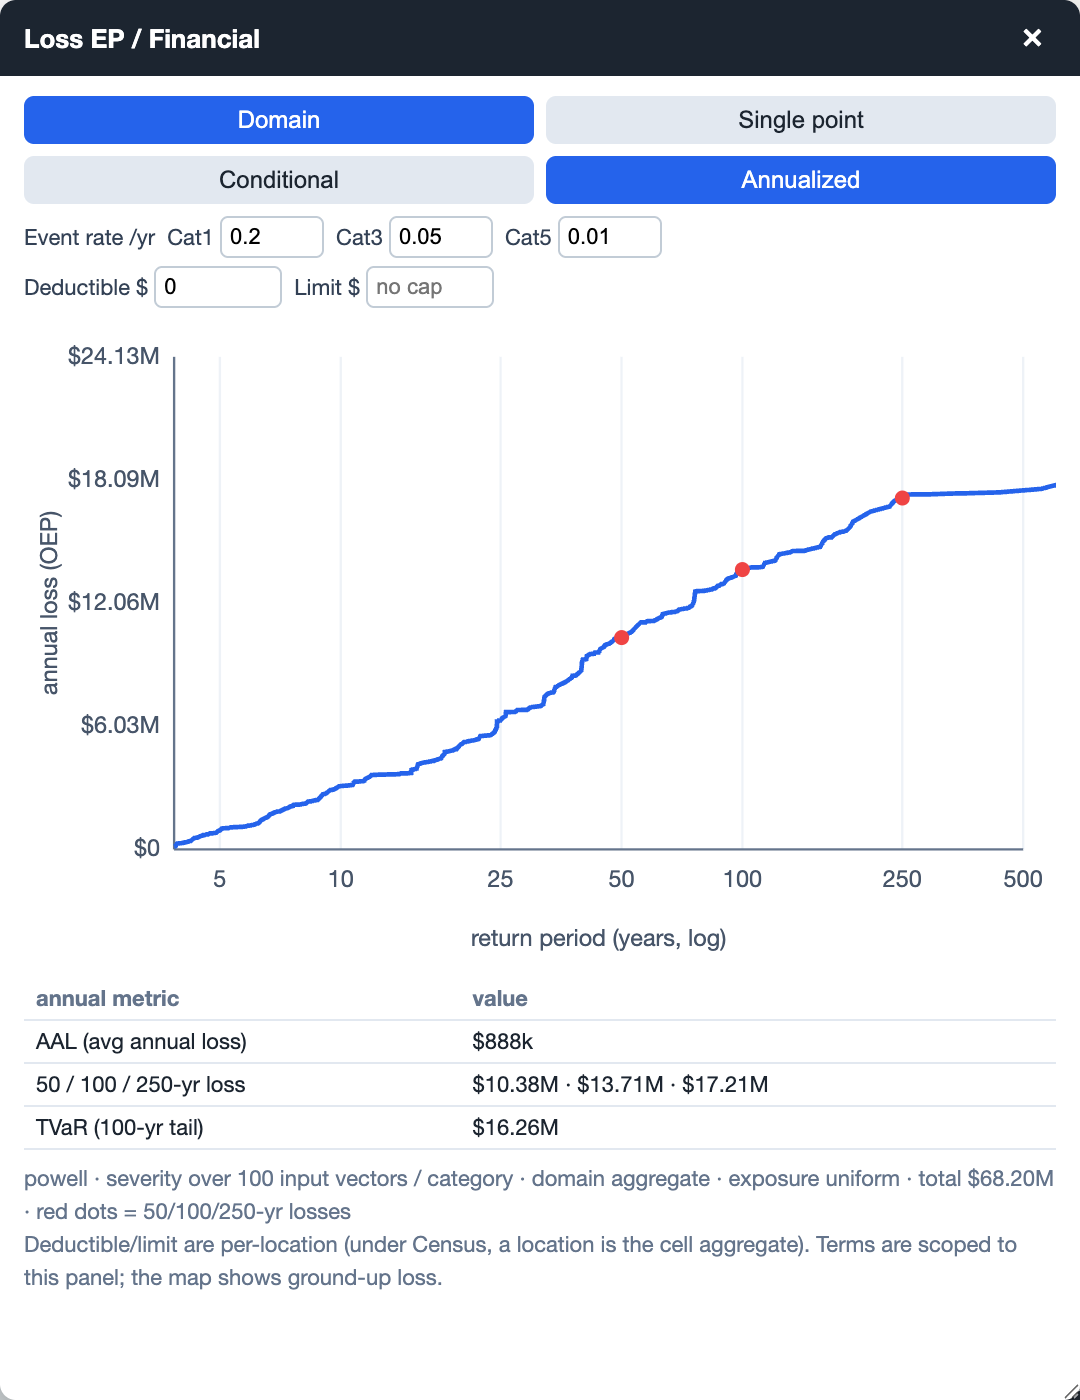
\includegraphics[width=0.62\textwidth]{analysis_financial.png}
\caption{Loss EP / Financial panel (annualized): the occurrence-exceedance-probability
curve of annual loss versus return period (red dots = 50/100/250-year losses), with
the editable event rates, deductible/limit, and the AAL / return-period / TVaR
metrics. Category~5 weighting shown; Powell.}
\label{fig:financial}
\end{figure}

\paragraph{Per-point EP and the AAL map (location-level loss).}
A second review comment asked to see the exceedance curve not only for the domain
aggregate but for an \emph{individual} grid point. A \textbf{Domain\,$\,\leftrightarrow\,$Single
point} toggle on the financial panel does this: in single-point mode the severity
samples are the loss at one map-picked vertex (shared with the profiler's pick)
rather than the $682$-vertex sum, and the identical conditional / annualized /
AAL / TVaR construction runs on them. The sampling is in fact the \emph{same} as
the aggregate---each point draws on the same $100$ Latin-hypercube vectors per
category; the aggregate does not use more storms, it averages over space---so the
per-point curve is no more thinly sampled than the domain curve (the $250$-year
point rests on the top one or two events in both). A companion map colouring,
\textbf{Annual loss (AAL~\$)}, paints every land vertex by its expected annual loss
$\mathrm{AAL}(x)=\sum_c \lambda_c\,\overline{L_c(x)}$ under the same rates and
terms, so the spatial variability of loss is visible at a glance
(Figure~\ref{fig:aalmap}). The important caveat is structural: because every
simulated storm follows the \emph{same} fixed due-west track and only the six storm
parameters vary, a point's loss distribution samples parameter uncertainty
\emph{only}, not landfall-location or heading uncertainty. Per-point AAL is
therefore biased (a vertex that always lies near the eyewall on this track is
overstated; a weak-quadrant vertex understated) and its variability is understated
relative to a track-sampled model. The per-point EP is thus \emph{scenario-
conditional}---``given these $100$ storms on this track''---and the panel says so;
read across points it is a faithful and useful picture of how loss varies over the
footprint under the ROA's fixed-track suite. (Because per-point loss reads the
precomputed peak-wind field rather than a live simulation, this works for every
wind model, including Powell and with Kaplan--DeMaria decay.)

\begin{figure}[H]
\centering
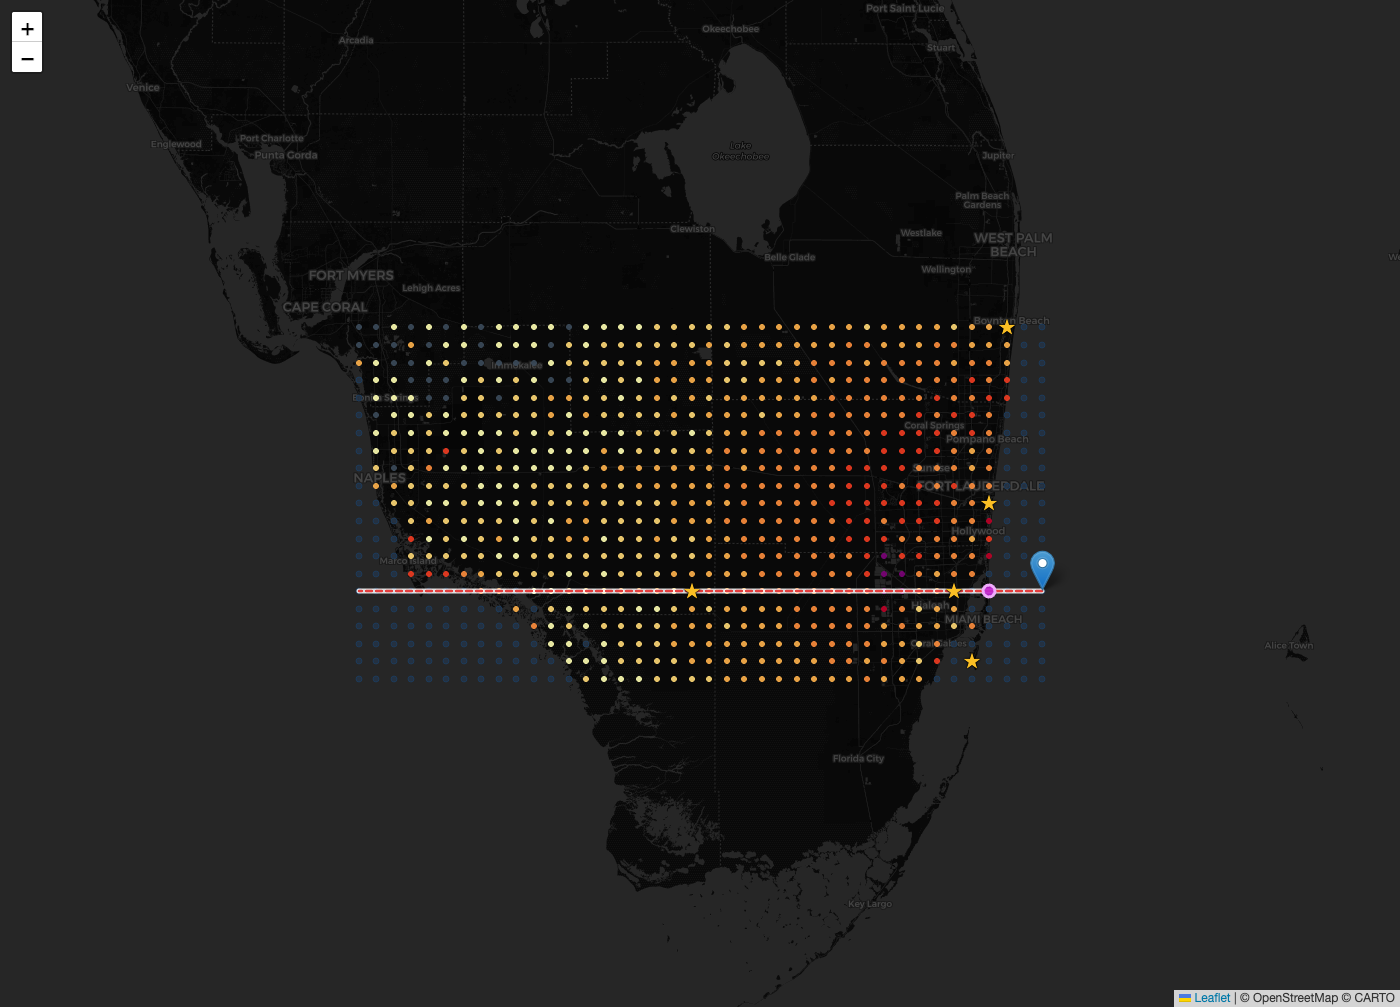
\includegraphics[width=0.82\textwidth]{aal_map.png}
\caption{Per-point expected annual loss (AAL, \$/yr) over the grid (Holland,
Uniform exposure, rates $\lambda=0.20/0.05/0.01$). Warmer points carry higher
annual loss; the hottest vertices lie along the storm track where the eyewall
passes, fading toward the weaker off-track quadrants. The pattern is scenario-
conditional on the fixed track (parameter uncertainty only).}
\label{fig:aalmap}
\end{figure}

The linear, second-order surface above is computed live in the browser. The
machine-learning metamodels below are instead fit offline and only evaluated in
the browser.

\subsection{Machine-learning metamodels (GPR and neural network)}
A \textbf{Metamodel} selector switches the profiler backend among three fits of
the same data: the live second-order \emph{Linear (RSM)} above, a
\textbf{Gaussian-process regression (GPR)}, and a \textbf{neural network}. The
latter two follow the deck's recommendation to go beyond first-order regression.
Both are fit with scikit-learn in \texttt{pipeline/fit\_metamodels.py}: the GPR
uses an anisotropic (automatic-relevance-determination, ARD) squared-exponential
kernel; the network is a two-hidden-layer perceptron ($6\times6$ tanh units,
L-BFGS, 5-fold cross-validated). To keep the deployed viewer a zero-backend static
page, training is done \emph{offline} for the default configuration (Powell +
surface roughness) per category and response; the fitted kernel hyperparameters /
weights are exported to \texttt{metamodels.json} and the browser only evaluates
them (a kernel dot-product for GPR, a forward pass for the network). The exported
parameters reproduce scikit-learn's own \texttt{predict} to within $10^{-9}$.

A \textbf{Compare} panel (Figure~\ref{fig:compare}) overlays the three
partial-dependence curves with an $R^2$ / cross-validated-$R^2$ table. Because the
Powell simulator is a smooth, deterministic function of the six inputs, all three
metamodels reach $R^2\approx1$ and their profiles nearly coincide; this agreement
is itself the result---three independent methods recovering the same main effects
and interaction curvature is strong evidence the structure is real, and confirms
that a second-order surface already suffices here. The added value of GPR/NN is
diagnostic rather than predictive: the GPR's ARD length scales rank the inputs by
influence, and its variance function yields Sobol \emph{total-effect} indices
$S_{T_i}$ (main effect plus all interactions involving $X_i$), which replace the
$\text{SRC}^2$ approximation in the EPR panel when GPR is selected. These recover
the ROA ordering---$S_{T_i}$ largest for WSP at Category~1 and for $R_{\max}$ at
Category~5.

\begin{figure}[H]
\centering
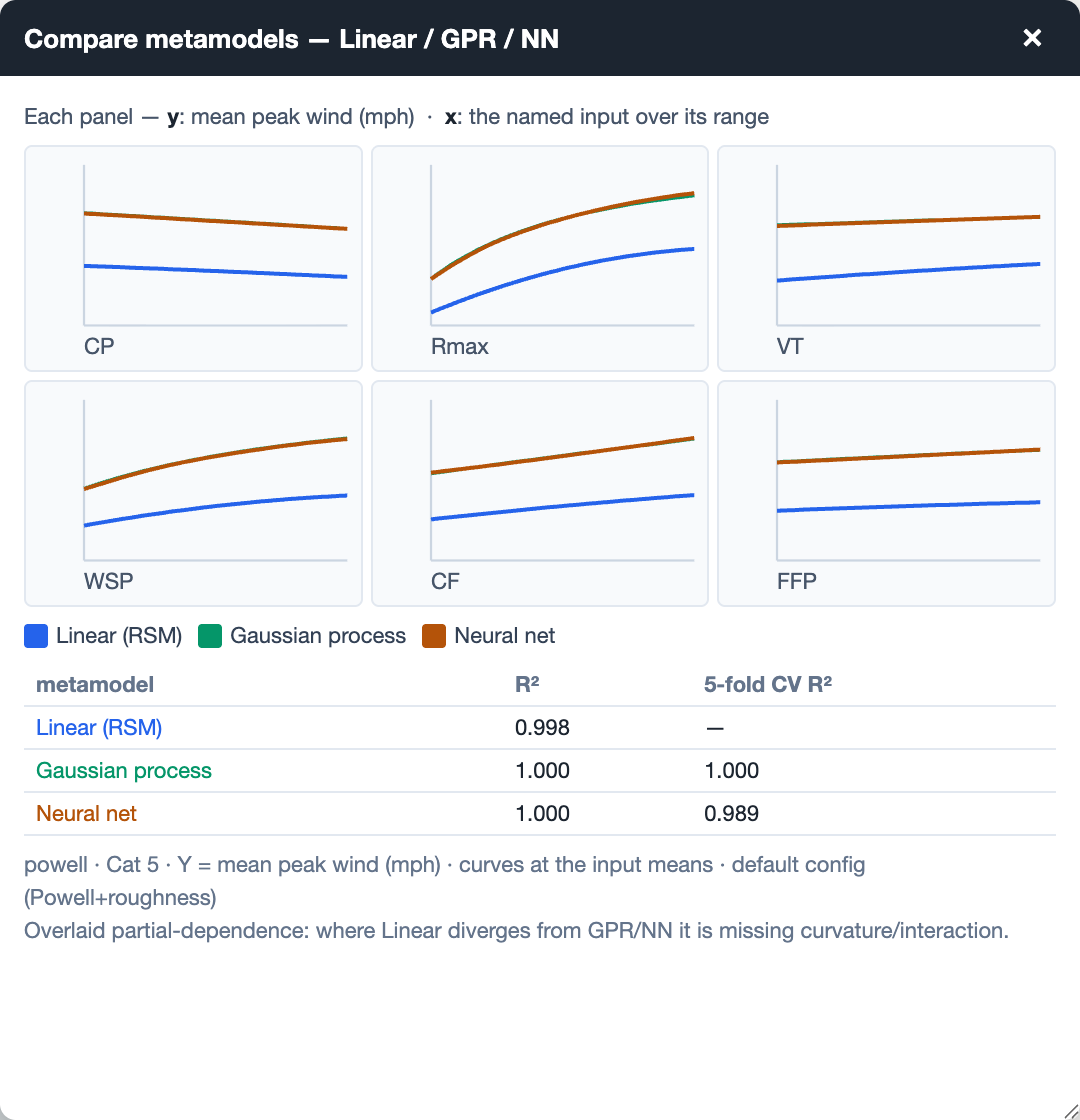
\includegraphics[width=0.72\textwidth]{analysis_compare.png}
\caption{Compare-metamodels panel: Linear (RSM), Gaussian process, and neural
network partial-dependence curves overlaid (Category~5, Powell), with the
$R^2$/cross-validated-$R^2$ table. The three nearly coincide---the agreement
validates the recovered effect/interaction structure.}
\label{fig:compare}
\end{figure}

\subsection{Grid-point-level sensitivity}
The SRC/EPR analyses above summarize the land-mean response. The deck also
recommends sensitivity \emph{at the grid-point level}, before averaging. The
\textbf{Sensitivity (dominant input)} colour mode does exactly this: at each land
vertex it regresses that vertex's peak wind over the 100 vectors on the six
standardized inputs and colours the vertex by its dominant input
(Figure~\ref{fig:gridsens}). The result is a spatial map of which storm parameter
controls the hazard where---e.g.\ for Category~1 the radius of maximum winds
$R_{\max}$ dominates the northern band while WSP dominates elsewhere---information
that a single grid-averaged table cannot convey.

\begin{figure}[H]
\centering
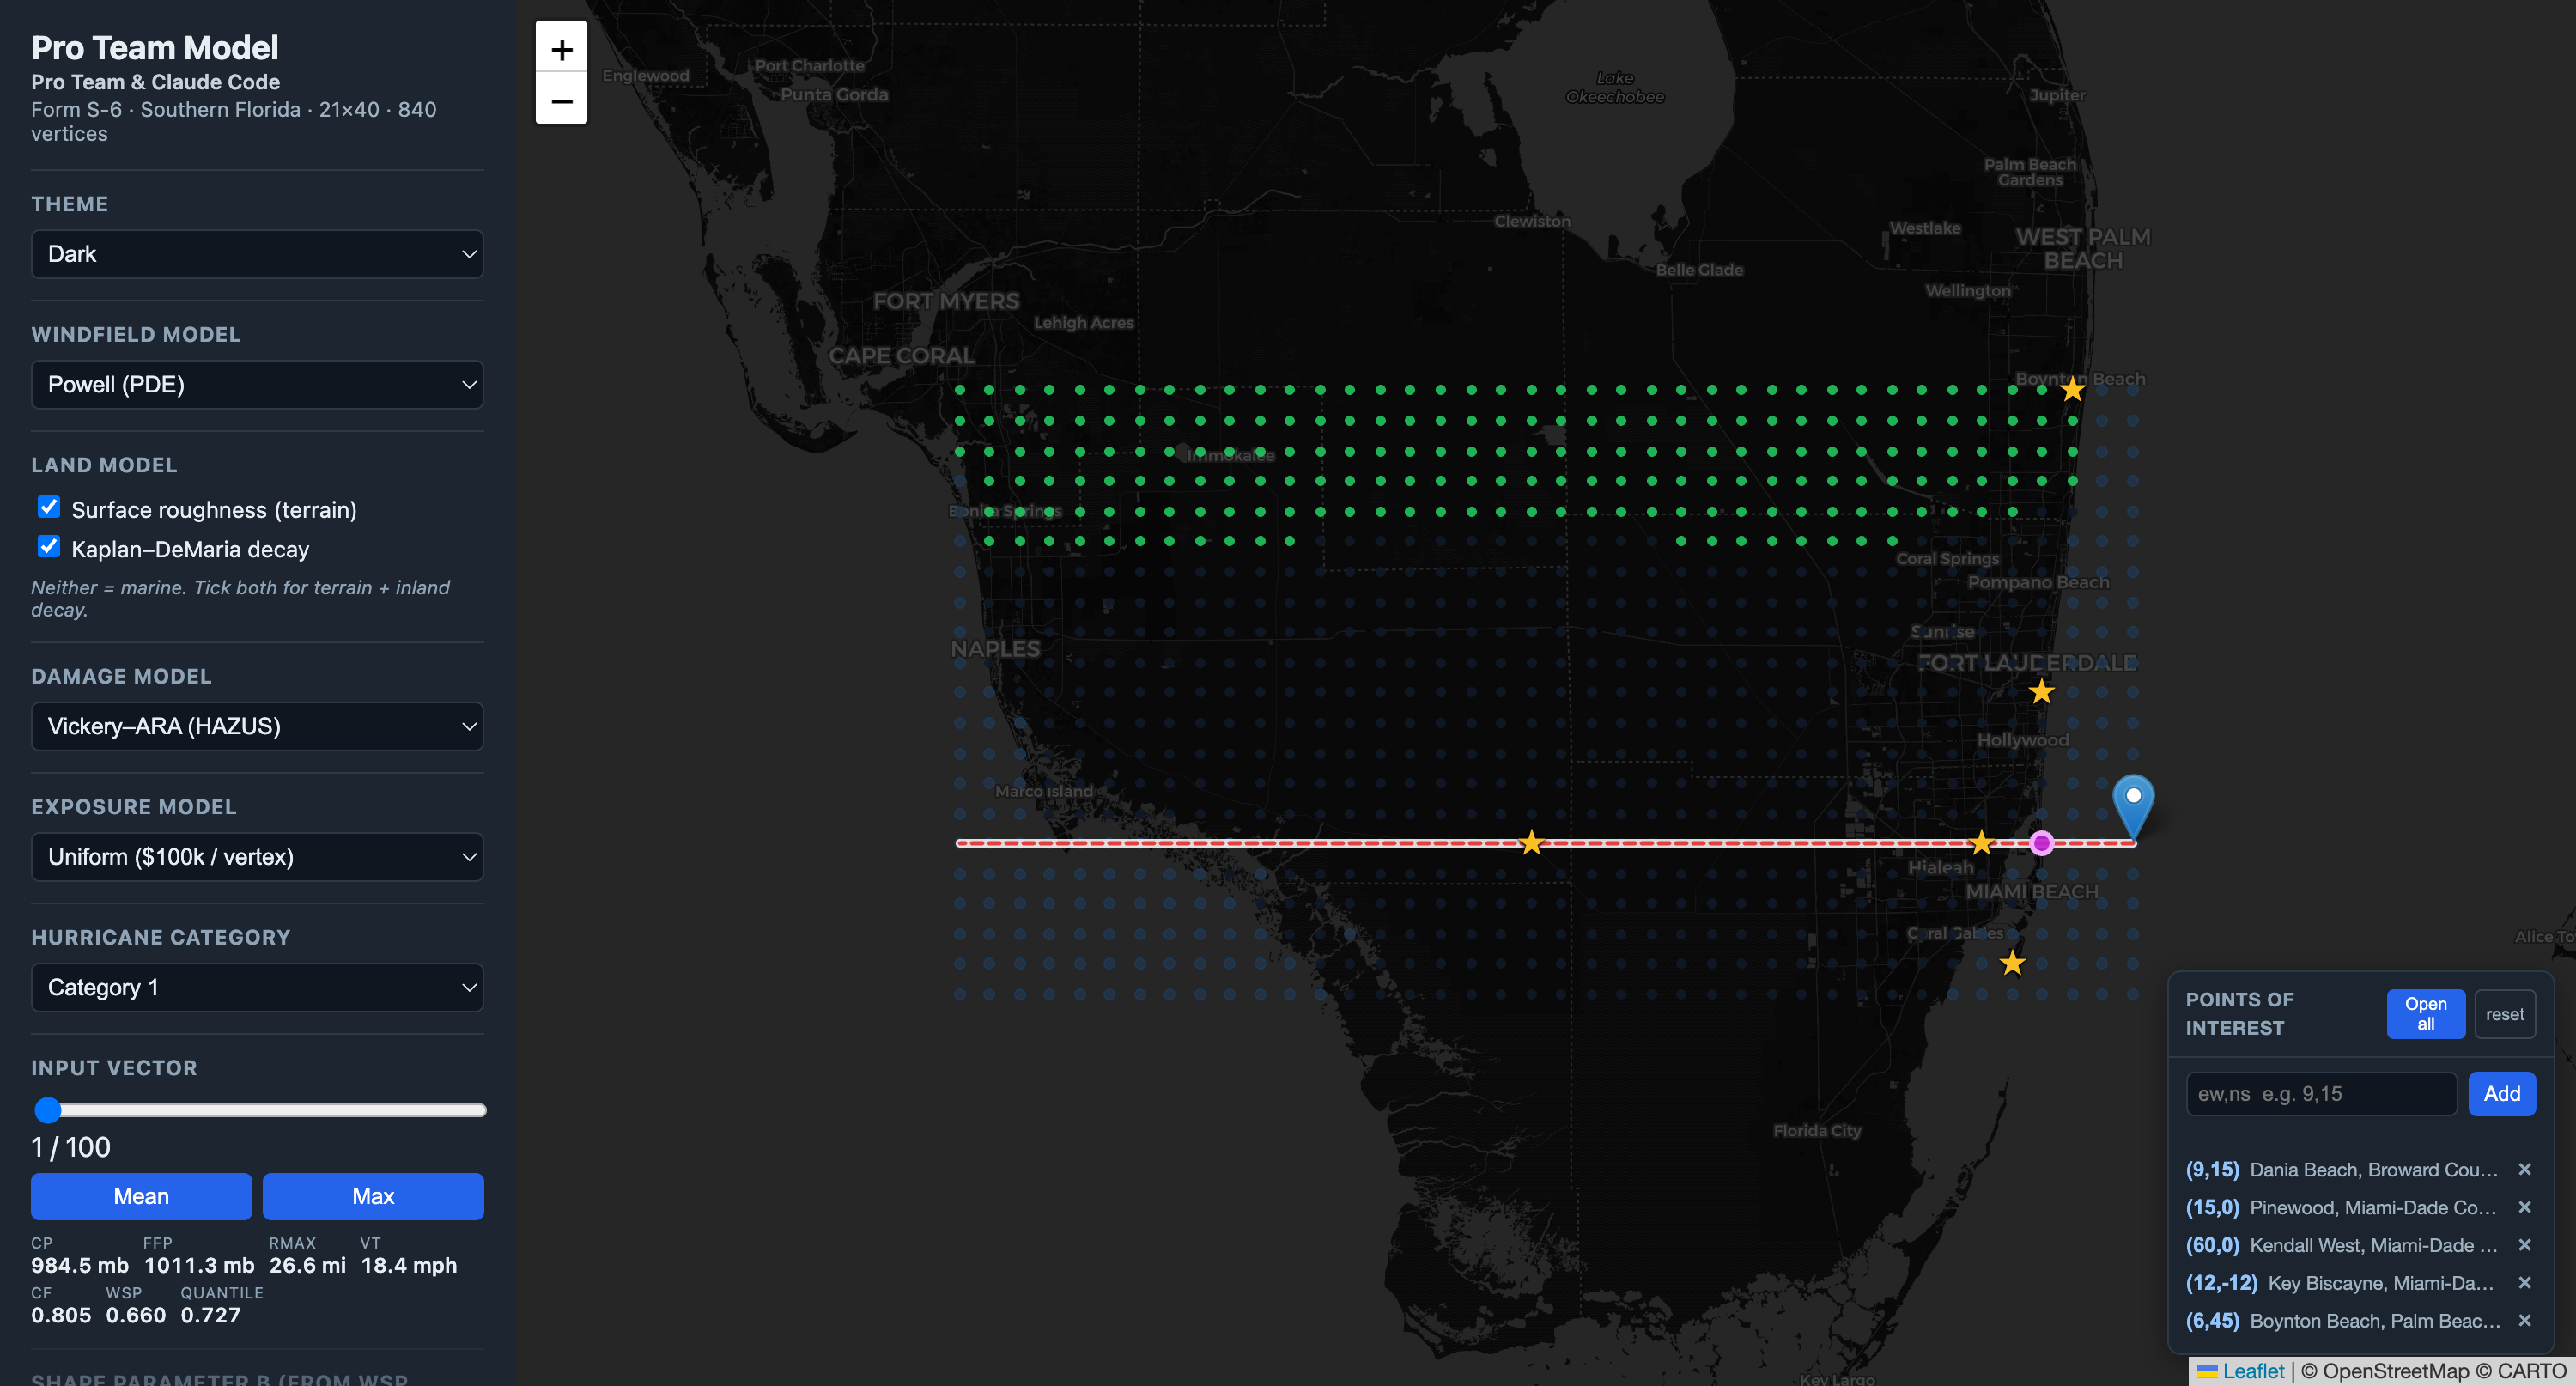
\includegraphics[width=0.8\textwidth]{grid_sensitivity.png}
\caption{Grid-point-level sensitivity (Category~1, Powell): each land vertex
coloured by its dominant input from a per-vertex standardized regression. The
dominant parameter varies spatially across the grid.}
\label{fig:gridsens}
\end{figure}

\section{Computer science: Interface and reproducibility}

\subsection{Design}\label{sec:design}
Before the interface itself, two diagrams fix the shape of the computation.
Figure~\ref{fig:dataflow} is the high-level data flow: land exposure enters on the
left, is modified by the land effects, and is then carried through the three
classical catastrophe-model stages---hazard, vulnerability, and loss costs.
Figure~\ref{fig:activity} refines that flow into a UML activity diagram, showing
the actual order of evaluation, the decision points at which a model is swapped,
and the loop over the 100 Form S-6 input vectors.

\begin{figure}[H]
\centering
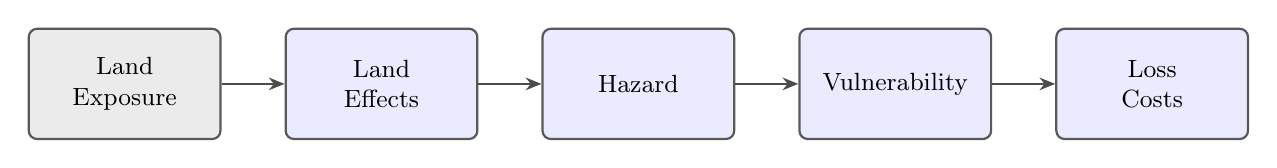
\begin{tikzpicture}[node distance=6mm and 8mm]
  \node[dfsrc]                  (exp)  {Land\\Exposure};
  \node[dfbox, right=of exp]    (land) {Land\\Effects};
  \node[dfbox, right=of land]   (haz)  {Hazard};
  \node[dfbox, right=of haz]    (vul)  {Vulnerability};
  \node[dfbox, right=of vul]    (loss) {Loss\\Costs};
  \draw[flow] (exp)  -- (land);
  \draw[flow] (land) -- (haz);
  \draw[flow] (haz)  -- (vul);
  \draw[flow] (vul)  -- (loss);
\end{tikzpicture}
\caption{High-level data flow. Exposure at the 682 land vertices is conditioned by
the land effects (surface roughness and Kaplan--DeMaria decay), which shape the
hazard (the wind field); the hazard drives vulnerability (the damage curve), and
vulnerability against exposure yields loss costs.}
\label{fig:dataflow}
\end{figure}

\begin{figure}[H]
\centering
\scalebox{0.74}{%
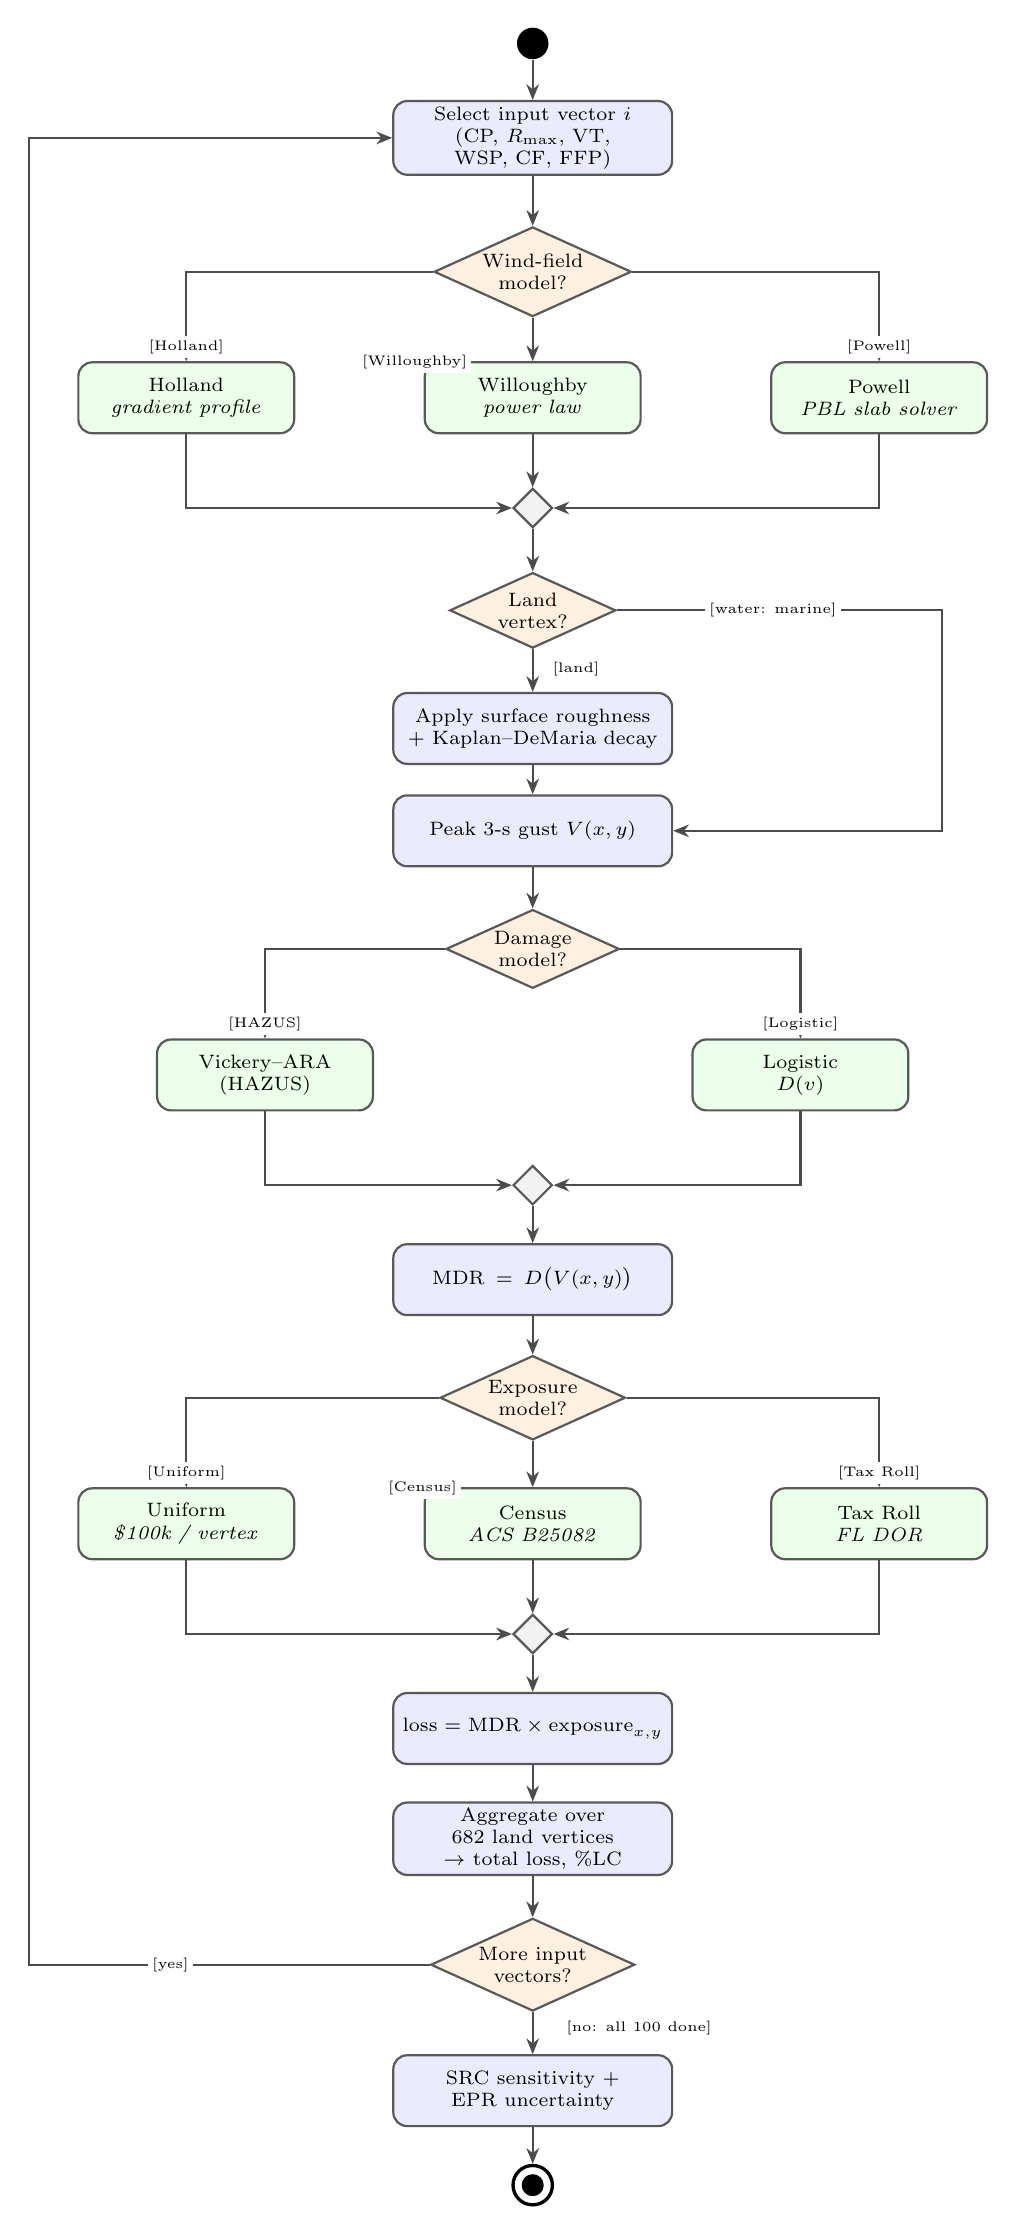
\begin{tikzpicture}
  % ---------------- Hazard ----------------
  \node[umlinit]  (start) at (0,0)      {};
  \node[umlact]   (pick)  at (0,-1.2)   {Select input vector $i$\\
                                         (CP, $R_{\max}$, VT, WSP, CF, FFP)};
  \node[umldec]   (dmod)  at (0,-2.9)   {Wind-field\\model?};
  \node[umlalt]   (hol)   at (-4.4,-4.5){Holland\\\emph{gradient profile}};
  \node[umlalt]   (wil)   at (0,-4.5)   {Willoughby\\\emph{power law}};
  \node[umlalt]   (pow)   at (4.4,-4.5) {Powell\\\emph{PBL slab solver}};
  \node[umlmerge] (m1)    at (0,-5.9)   {};
  \node[umldec]   (dland) at (0,-7.2)   {Land\\vertex?};
  \node[umlact]   (rough) at (0,-8.7)   {Apply surface roughness\\
                                         $+$ Kaplan--DeMaria decay};
  \node[umlact]   (gust)  at (0,-10.0)  {Peak 3-s gust $V(x,y)$};

  % ---------------- Vulnerability ----------------
  \node[umldec]   (dvul)  at (0,-11.5)  {Damage\\model?};
  \node[umlalt]   (haz1)  at (-3.4,-13.1){Vickery--ARA\\(HAZUS)};
  \node[umlalt]   (log1)  at (3.4,-13.1) {Logistic\\$D(v)$};
  \node[umlmerge] (m2)    at (0,-14.5)  {};
  \node[umlact]   (mdr)   at (0,-15.7)  {$\mathrm{MDR}=D\big(V(x,y)\big)$};

  % ---------------- Actuarial ----------------
  \node[umldec]   (dexp)  at (0,-17.2)  {Exposure\\model?};
  \node[umlalt]   (uni)   at (-4.4,-18.8){Uniform\\\emph{\$100k / vertex}};
  \node[umlalt]   (cen)   at (0,-18.8)  {Census\\\emph{ACS B25082}};
  \node[umlalt]   (tax)   at (4.4,-18.8){Tax Roll\\\emph{FL DOR}};
  \node[umlmerge] (m3)    at (0,-20.2)  {};
  \node[umlact]   (lc)    at (0,-21.4)  {$\text{loss}=\mathrm{MDR}\times
                                         \text{exposure}_{x,y}$};
  \node[umlact]   (agg)   at (0,-22.8)  {Aggregate over 682 land vertices\\
                                         $\rightarrow$ total loss, \%LC};
  \node[umldec]   (dmore) at (0,-24.4)  {More input\\vectors?};
  \node[umlact]   (stats) at (0,-26.0)  {SRC sensitivity $+$ EPR uncertainty};
  \node[umlfinal] (end)   at (0,-27.2)  {};

  % ---------------- Hazard edges ----------------
  \draw[flow] (start.south) -- (pick.north);
  \draw[flow] (pick.south)  -- (dmod.north);
  \draw[flow] (dmod.west)  -| (hol.north);
  \draw[flow] (dmod.south) -- (wil.north);
  \draw[flow] (dmod.east)  -| (pow.north);
  \node[guard] at (-4.4,-3.85) {[Holland]};
  \node[guard] at (-1.5,-4.05) {[Willoughby]};
  \node[guard] at (4.4,-3.85)  {[Powell]};
  \draw[flow] (hol.south) |- (m1.west);
  \draw[flow] (wil.south) -- (m1.north);
  \draw[flow] (pow.south) |- (m1.east);
  \draw[flow] (m1.south)    -- (dland.north);
  \draw[flow] (dland.south) -- (rough.north);
  \node[guard] at (0.55,-7.95) {[land]};
  \draw[flow] (rough.south) -- (gust.north);
  % water vertices keep marine winds: bypass the land effects
  \draw[flow] (dland.east) -- (5.2,-7.2) -- (5.2,-10.0) -- (gust.east);
  \node[guard] at (3.05,-7.2) {[water: marine]};

  % ---------------- Vulnerability edges ----------------
  \draw[flow] (gust.south) -- (dvul.north);
  \draw[flow] (dvul.west) -| (haz1.north);
  \draw[flow] (dvul.east) -| (log1.north);
  \node[guard] at (-3.4,-12.45) {[HAZUS]};
  \node[guard] at (3.4,-12.45)  {[Logistic]};
  \draw[flow] (haz1.south) |- (m2.west);
  \draw[flow] (log1.south) |- (m2.east);
  \draw[flow] (m2.south) -- (mdr.north);

  % ---------------- Actuarial edges ----------------
  \draw[flow] (mdr.south)  -- (dexp.north);
  \draw[flow] (dexp.west) -| (uni.north);
  \draw[flow] (dexp.south) -- (cen.north);
  \draw[flow] (dexp.east) -| (tax.north);
  \node[guard] at (-4.4,-18.15) {[Uniform]};
  \node[guard] at (-1.4,-18.35) {[Census]};
  \node[guard] at (4.4,-18.15)  {[Tax Roll]};
  \draw[flow] (uni.south) |- (m3.west);
  \draw[flow] (cen.south) -- (m3.north);
  \draw[flow] (tax.south) |- (m3.east);
  \draw[flow] (m3.south)  -- (lc.north);
  \draw[flow] (lc.south)  -- (agg.north);
  \draw[flow] (agg.south) -- (dmore.north);
  \draw[flow] (dmore.south) -- (stats.north);
  \node[guard] at (1.35,-25.2) {[no: all 100 done]};
  \draw[flow] (stats.south) -- (end.north);
  % loop back over the remaining input vectors
  \draw[flow] (dmore.west) -- (-6.4,-24.4) -- (-6.4,-1.2) -- (pick.west);
  \node[guard] at (-4.6,-24.4) {[yes]};
\end{tikzpicture}}
\caption{UML activity diagram for one evaluation pass. The three swappable model
families appear as decision nodes with guarded branches---wind field (hazard),
damage curve (vulnerability), and exposure (actuarial)---which is what makes the
app a \emph{multimodel}. Water vertices bypass the land effects and keep marine
winds. The outer loop repeats the pass for each of the 100 input vectors, after
which the SRC and EPR statistics of Section~\ref{sec:sa} are computed.}
\label{fig:activity}
\end{figure}

\subsection{Interface}
The viewer offers model / category / input-vector selection (the input vector
chooses one of the 100 randomized storms for the category), the WSP$\to B$
distribution control (which now reshapes only the live single-point profiler,
since all footprint windfields are precomputed at the default Uniform mapping),
the \textbf{Land model} checkboxes
(surface roughness and/or Kaplan--DeMaria decay, both on by default; neither =
marine), a colour-by control
(peak wind, loss MDR, land/water, or grid-point dominant-sensitivity), a
points/filled-contour display toggle,
light and dark themes (Figure~\ref{fig:light}; light is the default), and
nearest-point hover (peak wind, loss, coordinates, land/water, place name, and the
active input parameters).

\paragraph{One vector at a time.} The map always displays exactly \emph{one} input
vector, and the input-vector slider is always live. An earlier build opened instead
on a per-vertex field \emph{averaged over the 100 vectors}, with the slider
disabled. That view was withdrawn: averaging across vectors mixes 100 different
storms into a vertex value that no single storm ever produces, and it is not a
quantity the analysis ever asks for. The outputs of interest are aggregates over the
\emph{grid points} of a \emph{given} vector---above all $\mathrm{TLC}(i)$, the total
loss that storm $i$ inflicts over the domain. The Status panel therefore reports,
for the displayed vector, the total loss cost (in dollars and as a percentage of
exposure) together with the spatial mean and maximum of the peak wind over the 682
land vertices. This is exactly the quantity the sensitivity analysis regresses on:
the response $Y$ of Sections~\ref{sec:sa}--\ref{sec:sobol} is, and always was, a
per-vector aggregate over the grid points, so map and analysis now agree.

\textbf{Right-clicking}
a vertex exports a per-point loss-cost CSV for the current model/category/land-effect:
$100$ rows (one per input vector) by $9$ columns---the six Form S-6 inputs (CP,
$R_{\max}$, VT, WSP, CF, FFP), the peak wind at that vertex ($\mathrm{MaxWind\_mph}$),
and $\%\mathrm{LC}(i,x,y)=\mathrm{LC}(i,x,y)/\$100{,}000$
(the loss cost at that vertex) and $\%\mathrm{TLC}(i)=\mathrm{TLC}(i)/(\text{total
exposure})$, where $\mathrm{TLC}(i)=\sum_x\sum_y \mathrm{LC}(i,x,y)$ over all land
vertices. \textbf{Left-clicking} a vertex opens a floating windfield popup
(Figure~\ref{fig:popup}) with the storm-relative isotach field---the marked
vertex at its peak time---and that vertex's wind time series over the 12-hour
passage. The Sensitivity and Uncertainty results open as independent, movable,
resizable windows. Every plot the viewer draws---the analysis charts and the
windfield popup alike---supports mouse-wheel zoom about the cursor, drag-to-pan
once zoomed, and double-click to reset, for close inspection of individual curves.

\paragraph{Points of Interest.}
A panel in the lower-right of the map (Figure~\ref{fig:poi}) holds a list of named
\emph{points of interest}, addressed by their $(\mathrm{ew},\mathrm{ns})$
grid coordinate in miles; the user can insert any grid vertex (e.g.\ \texttt{9,15})
or delete an existing one, and the list persists across reloads. Five points are
provided by default---$(9,15)$, $(15,0)$, $(60,0)$, $(12,-12)$, $(6,45)$---each
shown as a star marker on the map. Clicking a point opens a detail page that
combines, for the current model/category, both the hover summary (peak/mean wind,
loss, coordinates, land/water, place name, and the active input parameters) and the
left-click windfield image (the storm-relative isotachs and the wind-vs-time series).
A \textbf{Print / Save PDF} button renders the page through the browser's print
dialog, so a point's report can be sent to a printer or saved as a PDF. An
\textbf{Open all} button assembles a single report page stacking every listed
point's summary and plots (one page-break per point), printable or savable as one
PDF. The panel itself is draggable by its header.

\begin{figure}[H]
\centering
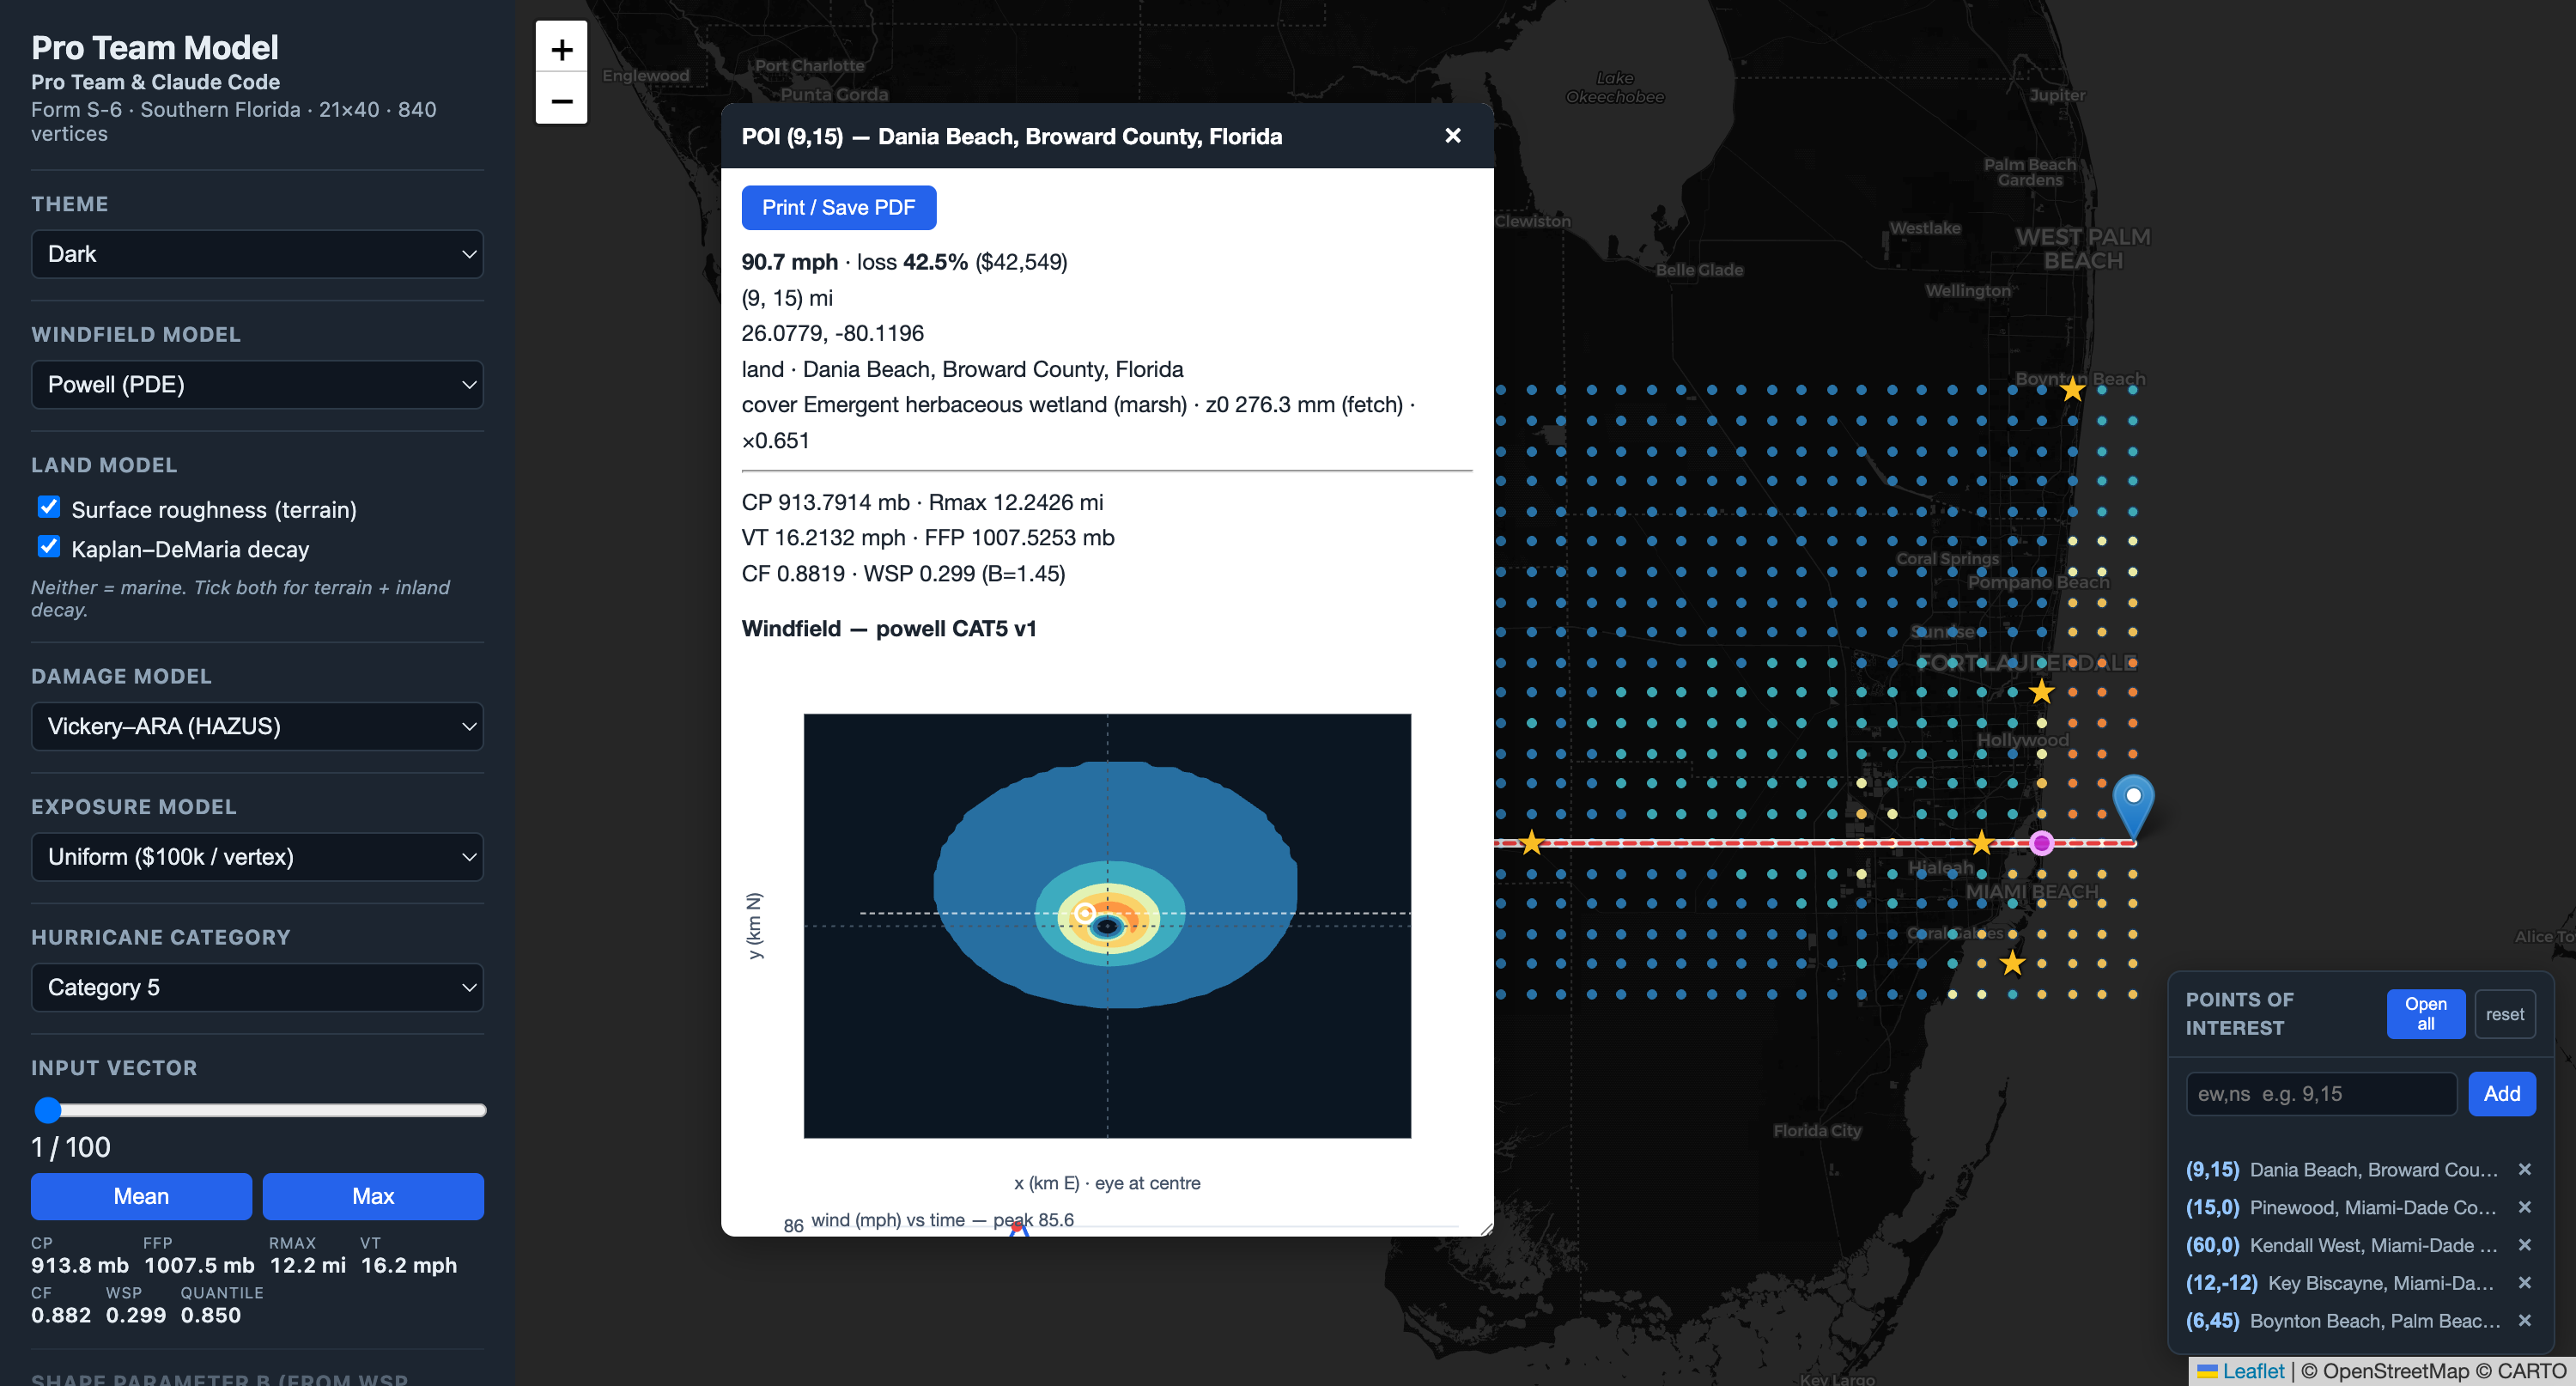
\includegraphics[width=\textwidth]{points_of_interest.png}
\caption{Points-of-Interest panel (lower right) with the five default points marked
as stars on the map, and the detail page for $(9,15)$---Dania Beach---combining the
hover summary, the storm-relative isotachs, and the wind-vs-time series, with a
Print / Save-PDF button.}
\label{fig:poi}
\end{figure}

\paragraph{Storm animation (optional).}
The static map colours each vertex by its \emph{peak over the whole passage}
(Section~\ref{sec:loss}); to also \emph{watch} the storm cross, an optional control
bar at the bottom of the map plays the \textbf{instantaneous} windfield as a
semi-transparent moving contour---the ground-frame view of the same field the
left-click popup shows storm-relative. It is off by default (the peak footprint
stays the default view) and nothing animates until the user presses Play or drags
the time slider ($t=-12\to+24$\,h); \textbf{speed} and \textbf{opacity} sliders set
the playback rate and how far the grid points show through the field. Two view
buttons choose the extent: \textbf{Narrow} (the default) renders only over the grid
at the default zoom, so the storm enters from the east edge near $t=0$ and the grid
points remain visible on top of the translucent bands and \emph{paint the footprint}
as the storm crosses. The precompute already simulated each storm sweeping east to
west (Section~\ref{sec:loss}: $\mathrm{ew}_c=V_T t$, keeping each vertex's peak over
$t=-12\to+24$); the animation replays that sweep, so the dots supply only its
\emph{time-varying build-up} while the magnitude is pinned to the static footprint:
each dot shows $\text{target}(x)\cdot\varphi(x,t)$, where $\varphi$ is the fraction of
the peak the storm has delivered at $x$ by time $t$ and $\text{target}$ is the field
the user already sees. Because $\text{target}$ is aggregation-aware
(\textbf{Mean}/\textbf{Max}/single vector), a vertex lights up when the eyewall
arrives, retains its value, and \emph{at $t=+24$ every dot equals the static footprint
exactly, in whatever mode is set} (Figure~\ref{fig:anim}, right);
\textbf{Wide} extends the render domain east into the Atlantic---sized per storm to
$12V_T+90$\,mi, since at $t=-12$ the eye is offshore ($\mathrm{ewc}=V_T t<0$)---and
zooms the map out so the full approach is visible (left). The storm then sweeps west,
the eyewall reaches the coast near $t=0$, and it clears the grid by $t=+24$; a moving
marker tracks the eye. All three wind models animate the selected input vector
(Holland/Willoughby live via the same field function as the time series; Powell by
sampling its stored storm-relative field), with surface roughness and
Kaplan--DeMaria decay applied per frame. Pressing Reset---or changing any sidebar
control---exits the animation and restores the static peak-wind footprint at the
default zoom.

\begin{figure}[H]
\centering
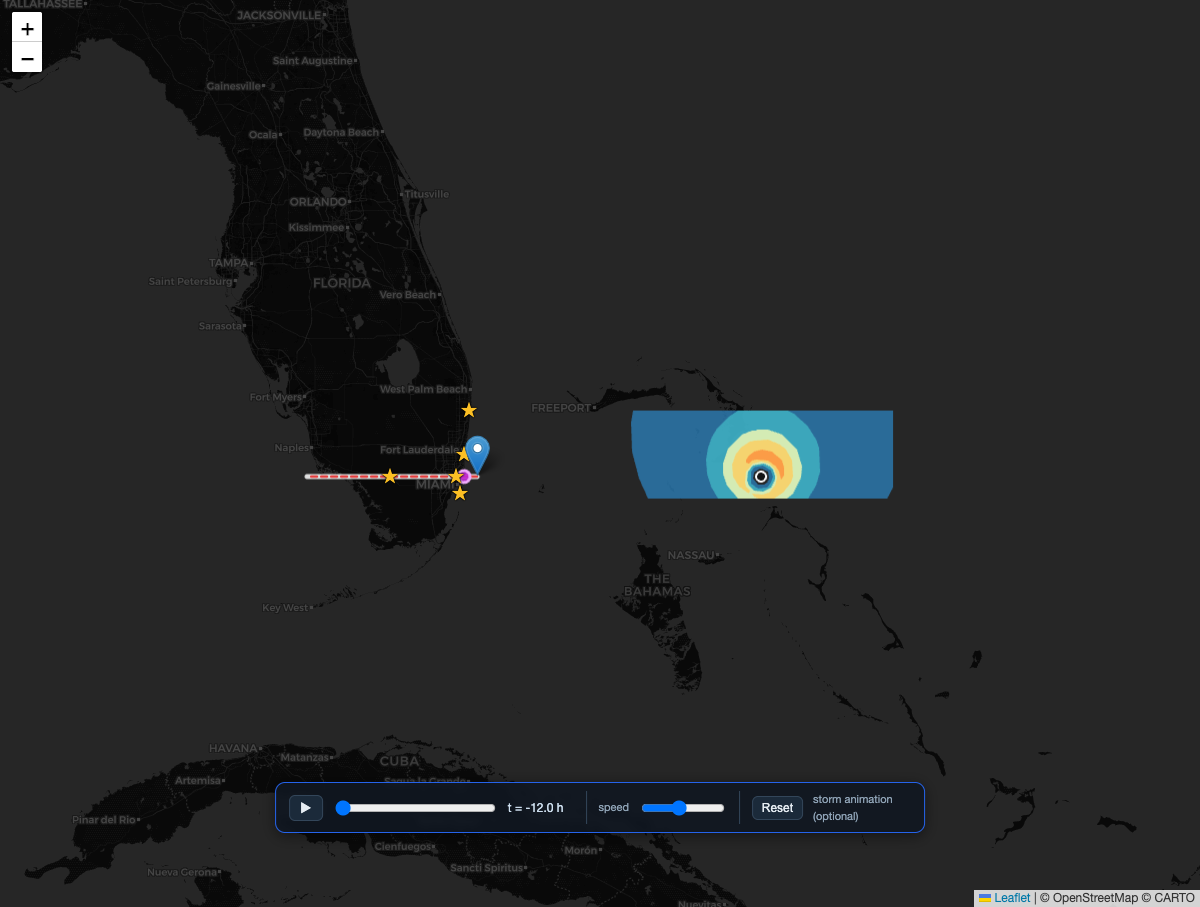
\includegraphics[width=0.49\textwidth]{anim_approach.png}\hfill
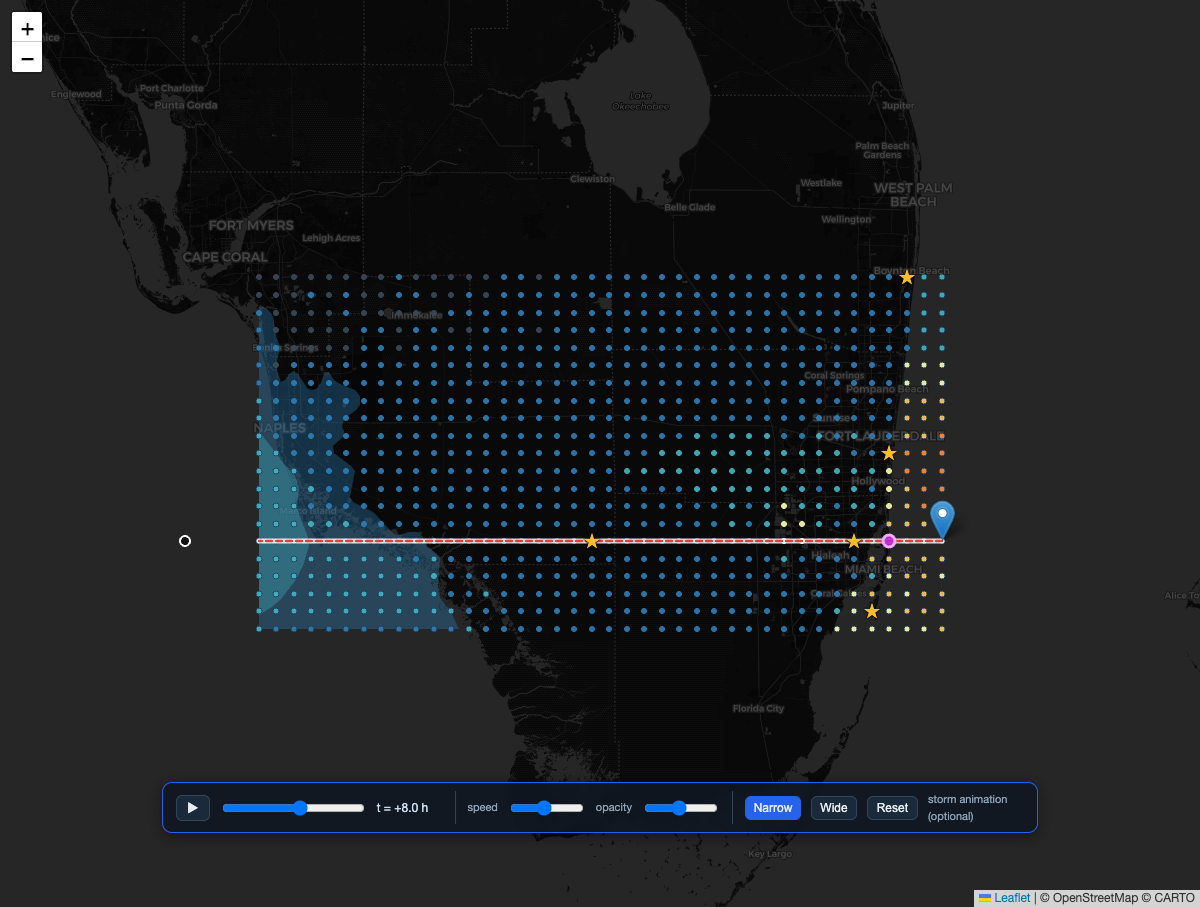
\includegraphics[width=0.49\textwidth]{anim_landfall.png}
\caption{Optional storm animation (Holland, Category~5). Left (\textbf{Wide}):
$t=-12$\,h---the instantaneous windfield offshore over the Atlantic as the storm
approaches, the map zoomed out over the extended domain. Right (\textbf{Narrow},
the default): mid-passage---the instantaneous storm (contour) has moved on while the
dots behind it have painted in their running-maximum wind (the peak footprint builds
up east-to-west and is retained; orange = strongest peak near the track). By $t=+24$
the dots equal the static peak-wind footprint. Speed / opacity sliders and
Narrow/Wide buttons sit on the control bar; Reset restores the static footprint at
the default zoom.}
\label{fig:anim}
\end{figure}

\begin{figure}[H]
\centering
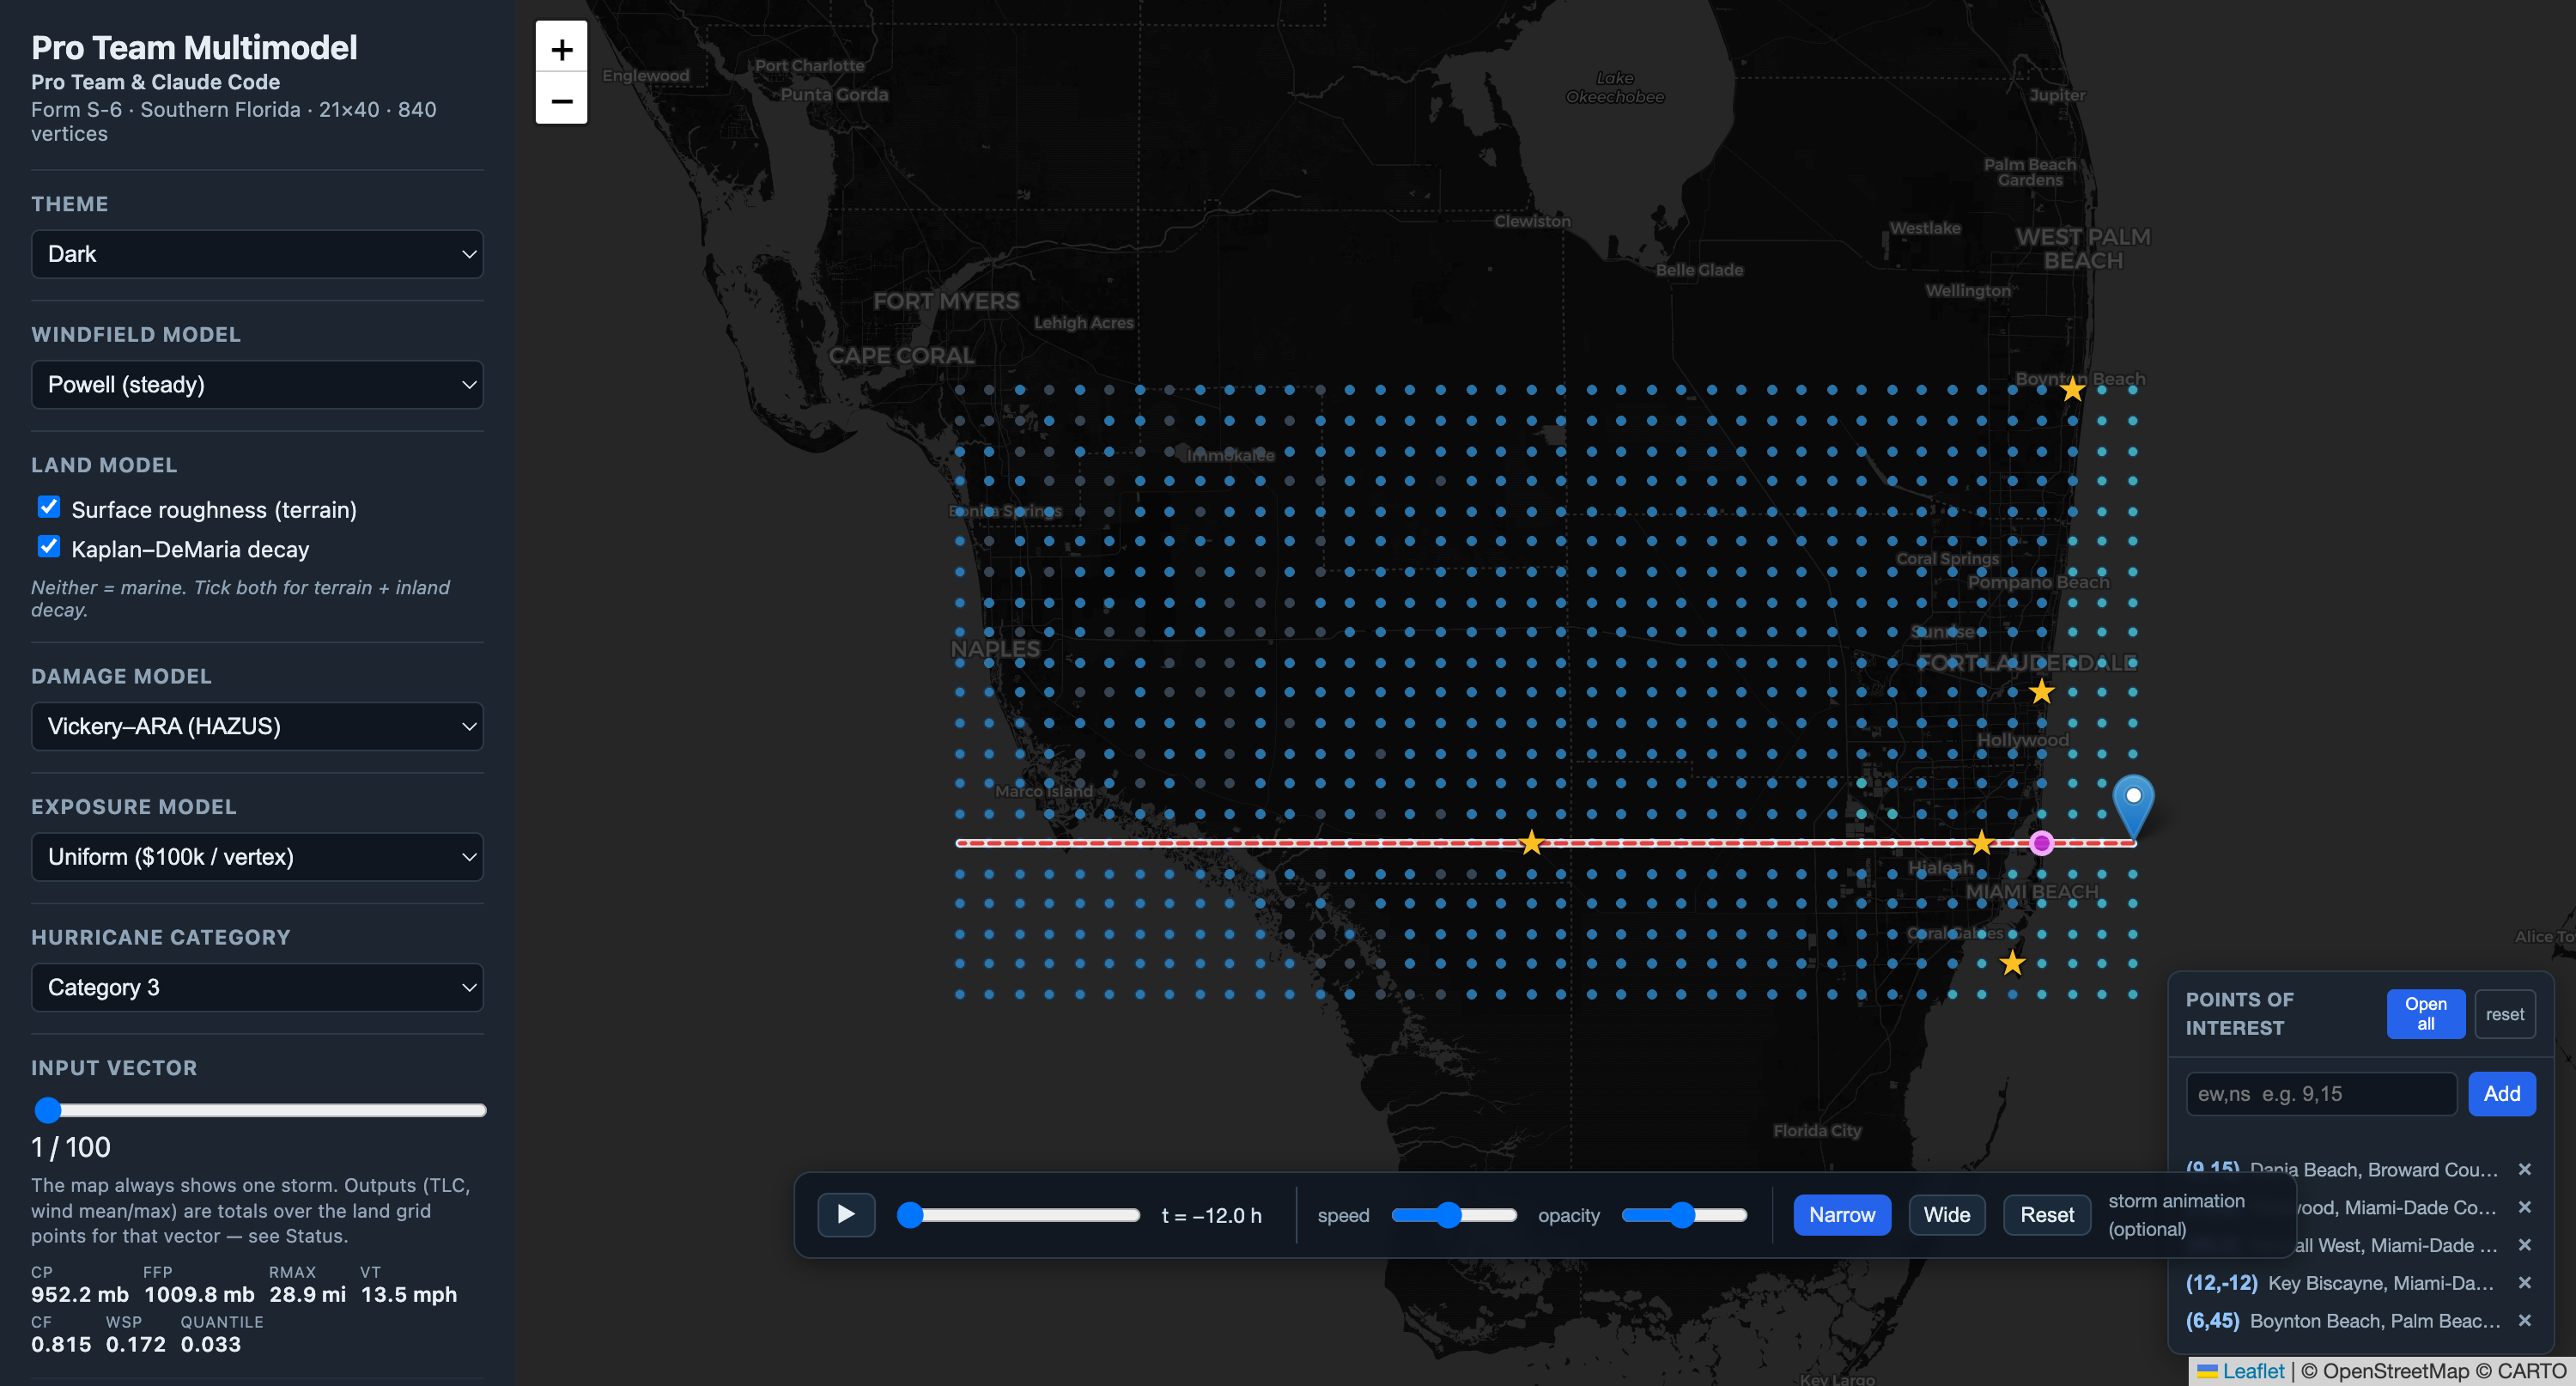
\includegraphics[width=0.46\textwidth]{dark_theme.png}\hfill
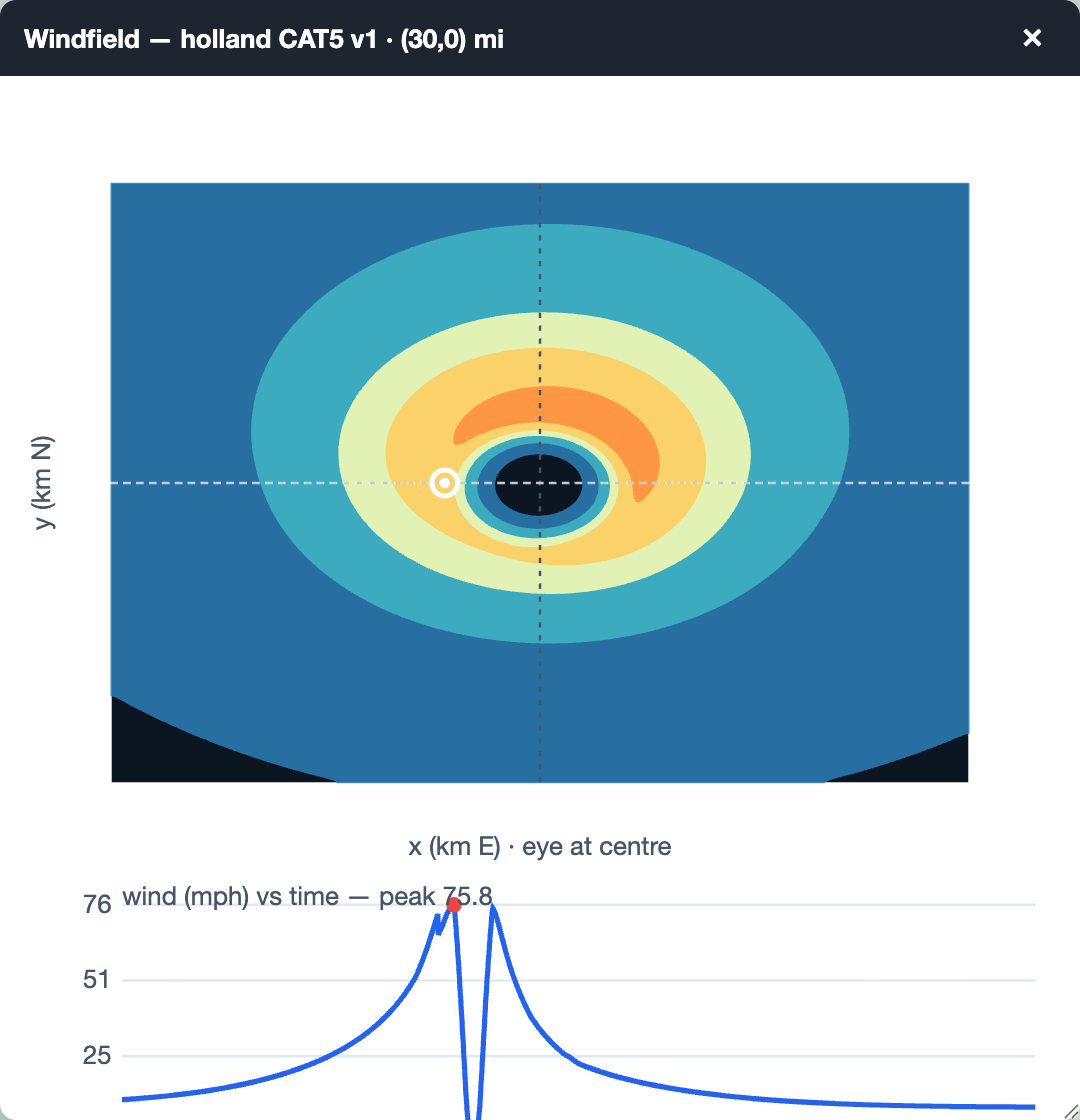
\includegraphics[width=0.46\textwidth]{windfield_popup.png}
\caption{Left: the optional dark theme, Powell Category~3 peak-wind points (the
viewer opens in the light theme used for every other figure here). Right: the
left-click windfield popup---storm-relative isotachs with the clicked vertex
marked at its peak time, plus the per-vertex wind time series.}
\label{fig:light}
\end{figure}
\label{fig:popup}

All data artifacts are reproducible via \texttt{pipeline/build\_all.sh}
(grid, place names, NLCD fetch, roughness, inputs, and the Powell
marine/K\&D/field precomputes), with \texttt{build\_vulnerability.py} for the
loss curve, \texttt{windfield\_ua.py} for the faithful Powell EPR, and
\texttt{precompute\_live.py} for the Holland/Willoughby footprint precomputes
(driven headlessly so they match the live field code exactly).

\paragraph{Serving and platform.}
The viewer is a self-contained client-side application (HTML/CSS/JavaScript with a
vendored copy of Leaflet under \texttt{web/vendor/}, so no content-delivery network
is required); its only runtime input is the precomputed JSON under
\texttt{outputs/web/}. Because the app loads that data with \texttt{fetch()}, which
browsers forbid under the \texttt{file://} scheme, it must be served over
\texttt{http://} from a local static server---double-clicking \texttt{index.html}
directly will not work. On macOS/Linux this is \texttt{./start} (a \texttt{zsh}
script running Python's \texttt{http.server}); for distribution to a
\textbf{Windows} machine without Python, \texttt{run.bat} launches an equivalent
zero-install server (\texttt{serve.ps1}, a PowerShell \texttt{TcpListener} on a
loopback port needing no administrator rights) and opens the browser. Both serve the
project root at \url{http://localhost:8012/web/index.html}. A runtime-only zip for
the Windows path (app, vendored Leaflet, and the \texttt{outputs/web/} data, without
the build-time virtual environment) is produced by \texttt{make-windows-zip.sh}. The
map's data layers render offline; only the basemap tiles require a network
connection.

Figures here are captured by \texttt{docs/capture\_figures.py} (Selenium driving
headless Chrome against the running viewer); the time-step convergence figure is
generated by \texttt{docs/make\_dt\_convergence.py}.

\section{Computer science: Verification and testing}\label{sec:verification}
Testing is done \emph{in the development loop} rather than as a separate phase: each
feature is landed together with an automated test that drives the running viewer and
asserts its behaviour, and the change is committed only once that test---and the
regression set around it---passes. The suite lives in \texttt{tests/auto/} and is run
with the project virtual environment against the local server (\texttt{./start}).

\paragraph{Automated UI suite.}
Twenty Selenium tests drive headless Chrome against the live page, exercising real
user actions (menu changes, button clicks, map picks, wheel/drag on plots) and
checking both the resulting state and that the browser console stays free of errors.
Coverage spans the interface and models (\texttt{check\_interface}), the mean/max
aggregation and filled contours (\texttt{test\_mean\_max\_buttons}), the exposure
models (\texttt{test\_exposure}), the per-point loss CSV (\texttt{test\_gridpoint\_csv}),
the Points-of-Interest panel (\texttt{test\_poi}), the input-vector row
(\texttt{test\_vec\_row}), plot zoom/pan/reset across every chart and the pop-up
(\texttt{test\_plot\_zoom}), the multiple simultaneous windfield pop-ups
(\texttt{test\_multi\_popup}), the metamodels and interaction profiler/matrix
(\texttt{test\_metamodels}, \texttt{test\_profiler\_cdf}, \texttt{test\_point\_response}),
the single-point responses (\texttt{test\_duration\_metric}, \texttt{test\_ike},
\texttt{test\_accloss}), the Powell per-vertex metamodel and the all-model
$\times$\,roughness/decay matrix (\texttt{test\_powell\_singlepoint},
\texttt{test\_singlepoint\_landcombos}), the per-point EP and AAL map
(\texttt{test\_point\_ep\_aal}), the financial panel (\texttt{test\_financial}), and
the storm animation (\texttt{test\_anim}). All twenty pass.

\paragraph{Consistency and invariant checks.}
The strongest verification is cross-checking independent code paths that must agree:
the live single-point simulation reproduces the \emph{precomputed} footprint at the
picked vertex to within $\sim$0.02\,mph for every roughness$\times$decay combination;
the storm animation's end state equals the static footprint \emph{exactly}
($682/682$ vertices) in Mean, Max, and single-vector modes; the per-point AAL summed
over land equals the domain aggregate AAL; the duration-accumulated loss is
calibrated so its 100-vector mean matches the peak-based \%LC (exactly), and its
sensitivity to $V_T$ is the opposite sign of the peak metric's; and the exported GPR
and neural-net metamodels reproduce scikit-learn's own \texttt{predict} to
$\sim\!10^{-9}$ (a parity check printed by \texttt{fit\_metamodels.py}).

\paragraph{Numerical / physics verification.}
Beyond the UI, the $\Delta t$ convergence study (\texttt{make\_dt\_convergence.py},
Figure~\ref{fig:dtconv}) confirms the 1-minute sampling resolves the peak; the
faithful Powell EPR is validated against the uncertainty-analysis worksheets; and
the track/contour rendering is checked in both themes
(\texttt{verify\_track\_contrast.py}). Client-side JavaScript is syntax-checked
(\texttt{node --check}) as part of each change.

\begin{thebibliography}{9}
\bibitem{fchlpm} Florida Commission on Hurricane Loss Projection Methodology (2025).
\emph{Report of Activities}. Standard S-3 and Form S-6.

\bibitem{iman} Iman, R.~L., Johnson, M.~E., and Schroeder, T.~A. (2001).
\emph{Professional Team Demonstration Uncertainty/Sensitivity Analysis}.
\url{https://fchlpm.sbafla.com/media/tepang2l/ua-sa-demo.pdf}

\bibitem{holland} Holland, G.~J. (1980). An analytic model of the wind and pressure
profiles in hurricanes. \emph{Monthly Weather Review}, 108, 1212--1218.

\bibitem{willoughby} Willoughby, H.~E., Darling, R.~W.~R., and Rahn, M.~E. (2006).
Parametric representation of the primary hurricane vortex. Part~II: A new family of
sectionally continuous profiles. \emph{Monthly Weather Review}, 134, 1102--1120.

\bibitem{powell} Powell, M.~D., Soukup, G., Cocke, S., Gulati, S.,
Morisseau-Leroy, N., Hamid, S., Dorst, N., and Axe, L. (2005). State of Florida
hurricane loss projection model: Atmospheric science component.
\emph{Journal of Wind Engineering and Industrial Aerodynamics}, 93(8), 651--674.
\url{https://www.aoml.noaa.gov/hrd/Powell/JWEIA1.pdf}

\bibitem{powell1996} Powell, M.~D., Houston, S.~H., and Reinhold, T.~A. (1996).
Hurricane Andrew's landfall in South Florida. Part~I: Standardizing the surface
wind observations. \emph{Weather and Forecasting}, 11, 304--328.

\bibitem{powellreinhold2007} Powell, M.~D., and Reinhold, T.~A. (2007).
Tropical cyclone destructive potential by integrated kinetic energy.
\emph{Bulletin of the American Meteorological Society}, 88(4), 513--526.

\bibitem{vickery} Vickery, P.~J., Wadhera, D., Powell, M.~D., and Chen, Y. (2009).
A hurricane boundary layer and wind field model for use in engineering applications.
\emph{Journal of Applied Meteorology and Climatology}, 48, 381--405.

\bibitem{hazus} Federal Emergency Management Agency (2025). \emph{Hazus 7.0
Hurricane Model Technical Manual}. FEMA. (Wind vulnerability methodology developed
by Applied Research Associates.)

\bibitem{vickery2006} Vickery, P.~J., Lin, J., Skerlj, P.~F., Twisdale, L.~A.,
and Huang, K. (2006). HAZUS-MH hurricane model methodology. II: Damage and loss
estimation. \emph{Natural Hazards Review}, 7(2), 94--103.

\bibitem{araoir2024} Applied Research Associates, Inc. (2024). \emph{2024
Residential Wind-Loss Mitigation Study} (Report \#005480). Prepared for the
Florida Office of Insurance Regulation, Tallahassee, FL.

\bibitem{kaplan} Kaplan, J., and DeMaria, M. (1995). A simple empirical model for
predicting the decay of tropical cyclone winds after landfall.
\emph{Journal of Applied Meteorology}, 34, 2499--2512.

\bibitem{esdu} ESDU (1985). \emph{Characteristics of atmospheric turbulence near the
ground. Part~II: Single point data for strong winds (neutral atmosphere)}. ESDU 85020.

\bibitem{nlcd} Multi-Resolution Land Characteristics Consortium (2023).
\emph{NLCD 2021 Land Cover (CONUS)}. \url{https://www.mrlc.gov}.

\bibitem{aersurface} U.S. Environmental Protection Agency.
\emph{AERSURFACE User's Guide}, land-cover to surface-roughness ($z_0$) tables.

\bibitem{smithvogl} Smith, R.~K., and Vogl, S. (2008). A simple model of the
hurricane boundary layer revisited. \emph{Quarterly Journal of the Royal
Meteorological Society}, 134, 337--351.

\bibitem{francom} Francom, D., and Nachtsheim, A. (2025). \emph{A Review and
Comparison of Different Sensitivity Analysis Techniques in Practice}. Los Alamos
National Laboratory. arXiv:2506.11471.

\bibitem{sobol} Sobol', I.~M. (2001). Global sensitivity indices for nonlinear
mathematical models and their Monte Carlo estimates. \emph{Mathematics and
Computers in Simulation}, 55, 271--280.

\bibitem{saltelli2010} Saltelli, A., Annoni, P., Azzini, I., Campolongo, F.,
Ratto, M., and Tarantola, S. (2010). Variance based sensitivity analysis of model
output. Design and estimator for the total sensitivity index. \emph{Computer
Physics Communications}, 181, 259--270.

\bibitem{jansen1999} Jansen, M.~J.~W. (1999). Analysis of variance designs for
model output. \emph{Computer Physics Communications}, 117, 35--43.
\end{thebibliography}

\end{document}
